\documentclass[pdftex,12pt,a4paper]{article}

\usepackage[pdftex]{graphicx}
\usepackage[english]{babel}
\usepackage[utf8]{inputenc}
\usepackage{amsmath}
\usepackage{graphicx}
\usepackage[colorinlistoftodos]{todonotes}
\usepackage[margin=1in]{geometry}
\usepackage{float}
\usepackage{listings}
\usepackage{units}
\usepackage{hyperref}
\usepackage{enumitem}
\usepackage{textcomp}
\usepackage{setspace}
\usepackage{cite}



\newcommand{\HRule}{\rule{\linewidth}{0.5mm}}
\singlespacing
%\onehalfspacing
%\doublespacing

\title{Clinic Final Report}
\begin{document}

\begin{titlepage}

\vspace*{\fill}
\begin{center}

\textsc{\Large Clinic Final Report}\\[1.5cm]

% Title
\HRule \\[0.4cm]
\begin{figure}[h]
  \centering
    
\includegraphics[scale=2.80]{HRL_logo.jpg}
\end{figure}

\HRule \\[1.5cm]



\begin{minipage}[t]{0.4\textwidth}
    \begin{flushleft}
        \large \textit{Students}:\vspace*{0.3cm} \\
        Paul Jerger \\
		Alex Kendrick\\
		Kunal Menda\\
		Nithya Menon\\
		Fernando Ortega\\
		Luke St Marie\\
    \end{flushleft}
\end{minipage}%
%
\begin{minipage}[t]{0.4\textwidth}
    \begin{flushright}
        \large \textit{Advisors}:\vspace*{0.3cm} \\
        Prof. Qimin Yang\\
		Prof. Theresa Lynn\\
        \vspace*{0.5cm}
        \large \textit{Liaisons}:\vspace*{0.3cm} \\
        Thaddeus Ladd `98\\
        Danny Kim\\
        Matthew Rakher\\
        Cody Jones
    \end{flushright}
\end{minipage}%

\vfill

% Bottom of the page
{\large May 1, 2015}

\end{center}

\vspace*{\fill}

\end{titlepage}

\doublespacing

\tableofcontents

\newpage
\begin{abstract}
The Harvey Mudd clinic team sponsored by HRL Laboratories has been tasked with designing, evaluating, and modeling optical networks to generate sequences of ultrafast optical pulses on a time scale of 300 to 3000 nanoseconds. The Mid-year Report summarizes the team's conceptual design process, presents a detailed version of the chosen design, and describes the ongoing simulation and modeling work. Based on the flexibility in pulse arrival times which the design must accommodate, the team has created a design which digitizes the possible pulse arrival times. The design sacrifices precision for adaptability, the consequences of which are also modeled. In the spring semester, the team will physically model key aspects of the design and continue to model its non-ideal behavior in order to justify the digitizing approach.
\end{abstract}

\section{Introduction}
HRL Laboratories is sponsoring a 2014-15 Clinic Project to develop optical network designs to produce a precisely timed laser pulse sequence for delivery to a quantum dot. This section describes HRL Labs, presents the project statement, defines the deliverables for the project, and describes the status of the project to date.

\subsection{HRL Laboratories}
HRL Laboratories was founded in 1948 and is recognized as one of the world’s premier physical science and engineering research facilities. One of HRL Lab’s first great achievements was the demonstration of the world’s first laser, in 1960. They are leaders in the field of integrated circuits, designing custom optical fibers and integrated optical circuits. 
HRL Laboratories aims to make an impact in the field of quantum communication, and to that end is researching systems in which the electron spin of a quantum dot is used as quantum memory. One significant difficulty of this system lies in electron spin states decohering rapidly. Delivering specific time sequences of ultrafast laser pulses can increase control over an electron’s spin. However, the ultrafast nature of the pulses severely limits the range of feasible designs. Optical systems that deliver such precisely timed sequences have so far been prohibitively expensive and limited to simple pulse sequences. This clinic project focuses on designing and evaluating low-cost optical systems which can create more complex pulse sequences. Having such optical systems would allow researchers to explore novel pulse sequences which might prove more effective in extending the lifetime of quantum information.

\subsection{Project Statement}
The 2014-2015 HRL Clinic team will design, evaluate, and model systems of optical components to deliver precisely timed series of ultrafast laser pulses for use in electron spin manipulation.

\subsubsection{Objectives}
Objectives for the optical network designs include:
\begin{itemize}
\item Reduce cost and number of optical components
\item Be adaptable for different pulse sequence lengths and time spans
\end{itemize}

\subsubsection{Constraints}
The design must meet the following constraints:
\begin{itemize}
\item Fit on the 4’ x 5’ optical table
\item Utilize the single laser wavelength, between 920 and 930 nanometers
\item Maintain 2-3 picoseconds precision on pulse spacing
\item Maintain the required polarization and intensity of the light incident on the quantum dot
\end{itemize}

\subsubsection{Functions}
The optical network design should perform the following functions to optimize spin control:
\begin{itemize}
\item Delay laser pulses
\item Select laser pulses
\item Attenuate laser pulses
\end{itemize}

\subsection{Deliverables}
By the end of the fall semester, the team has completed and will deliver:
\begin{itemize}
\item Designs for optical network schematics
\item A simulation tool for analyzing a potential optical network
\item Preliminary metrics for evaluating the quality of pulse sequences
\item Project documentation and presentations including:
\begin{itemize}
\item Work Plan
\item Mid-year Report
\item Three internal design review Clinic presentations
\end{itemize}
\end{itemize}
By the end of the spring semester, the team will deliver:
\begin{itemize}
\item Detailed designs of thoroughly tested optical networks (both feasible and not)
\item Component purchase recommendations for detailed designs
\item Experimental procedure outline for complex designs
\item Further developed simulation tools for pulse sequence analysis
\item Project documentation and presentations including:
\begin{itemize}
\item Final Report (including engineering drawings)
\item Spring semester presentation at HMC
\item Projects Day presentation
\item Final Presentation at HRL Laboratories
\end{itemize}
\end{itemize}

The fall deliverables in the Work Plan originally called for results from initial experimentation on design alternatives. However, the designs that the team initially developed involved a straightforward use of passive components that did not require much experimental validation. The team is now pursuing more complex designs that will require testing either in partial, using subsets of the design's components, or in full, using the whole design but at slower speeds. In addition, the procedure for setting up the entire experiment is nontrivial, so the spring deliverables include testing for the purposes of both validating the concepts of the design and determining a logical experimental procedure.

\subsection{Project Status}
The team has completed all of its fall deliverables. The team formulated three broad categories of conceptual design, which are described and evaluated in Section \ref{sec:design_alternatives}. Of these alternatives, the team chose the most promising - a digitization paradigm - and created a detailed design, which is explained in Section \ref{sec:detailed_design}. In order to validate the conceptual design and model physical imperfections, the team wrote computational simulations in Simulink and other analysis software, which are covered in Section \ref{sec:results}. This section contains the existing results and their effect on the project thus far, and Section \ref{sec:test_plan} outlines future simulation and physical experiment plans. Section \ref{sec:project_managment} places future work on a projected timeline for the spring semester.




\section{Impact}
The developing field of quantum information is a relatively young area of physics with the potential to significantly advance current communication and computation technology. Currently, information is represented as strings of bits, where each bit is either a one or zero, in order to perform computations or transmit data; this is also known as a “classical” system. Quantum information science, on the other hand, uses quantum bits - “qubits” for short - which can be in superpositions of the states of the classical bit. This property of superposition is the quantum aspect of the qubit, and allows individual qubits (and systems composed of them) to manipulate information that classical bits cannot. However, while the theoretical capabilities of systems of qubits have been well-described, the experimental field has yet to achieve many of the theoretical results.

This clinic project is part of ongoing research in the field of quantum information - both at HRL Laboratories and elsewhere - on qubit systems. The ultimate goal of these research efforts is to produce a feasible quantum communication network, composed of a large number of qubits and functional over long distances. There is a long way to go before such a system can be constructed due to a number of technical hurdles. These difficulties include: qubits take a lot of equipment to maintain, such that systems of large numbers of qubits are currently unfeasible; qubits decohere too quickly to allow for transmission over long distances; qubit states cannot be copied like classical bits, and cannot be read out without changing the state (theoretical obstacles that must be worked around in the implementation); and quantum gates are more complex than their classical equivalent.

The problem set by HRL Laboratories for the clinic team addresses the decoherence issue for a specific qubit system, that is, a single-electron spin trapped in a quantum dot. A satisfactory conclusion to the clinic project would still be very far removed from realizing a fully-functional, large-scale quantum communication network, but it would provide necessary experimental verification for theoretical results, and may potentially advance the current state of quantum-dot spin qubits by increasing decoherence time. Furthermore, the clinic team may also develop optical network designs that become useful beyond the specific application commissioned by HRL Laboratories.

In the big picture, well beyond the scope of this project, quantum information technology has a lot of theoretical impact to make on society. It has long been known that RSA encryption would be endangered by an efficient quantum computer, since RSA relies on the classical difficulty of factoring an extremely large number into primes. Shor's factoring algorithm for a quantum computer is much more efficient than the classical analogue; thus a quantum computational system would be able to break RSA encryption. New quantum communication security protocols would need to be developed in turn. Cryptography is therefore an important application of quantum computers and quantum communication protocols. Beyond that, quantum computing can offer possible improvements on the computation time of NP-complete problems and search algorithms \cite{nielsen_michael_a._quantum_2000}, which can be applied to a wide variety of situations. Another intriguing application of fully-quantum computational tools would be the ability to use those systems to exactly simulate other fully-quantum systems, which classical computers will always have to approximate numerically. However, until satisfactory qubit systems are developed, these applications are largely theoretical results.




\section{Background}
\subsection{Quantum Communication Networks} 

One of the great challenges of developing a quantum communication system, or a quantum computer, is creating a physical realization for a system of qubits. The physical model must exhibit quantum properties while at the same time it needs to be easily manipulated so that it can perform computations. The issue arises from the fact that most physical realizations that exhibit quantum mechanical effects tend to be atomic in size, making manipulation of the system difficult and information loss due to local environmental interactions a real concern. 

Some proposed forms for a qubit involve the manipulation of the single electron spin in a semiconductor quantum dot. A quantum dot is semiconductor crystal that traps an electron, or hole, in a potential well with discrete states. In this case the orientation of the electron’s spin would encode a qubit since spin-up or spin-down states can be related to a one or zero. The qubit can then be processed (read or overwritten) by using laser pulses to manipulate the electron spin.

The experiments at HRL Laboratories will make use of Indium Gallium Arsenide/Gallium Arsenide (InGaAs/GaAs) semiconductor quantum dots contained within a uniform magnetic field. The problem with such a qubit system is the fact that the electrons’ spin orientations will dephase due to the electromagnetic interactions with the local background magnetic field. The time for the dephasing of the spin orientation, known as the decoherence time, is on the order of a few nanoseconds which is undesirable for information processing if one intends to perform computations with the quantum dots. One way of extending this decoherence time is by using dynamical decoupling methods, which essentially involves using ultrafast pulse sequences to prevent the dephasing of the electron. By constantly manipulating the electron spin with these pulse sequences it is possible to refocus the spin enough to extend the decoherence time to something on the order of microseconds, which is a much more workable timescale for information processing\cite{Nuclear_Feedback}.

\subsection{Electron Spin Manipulation and Decoherence} 
In a quantum dot, the electron spin will precess naturally if it is placed in an external magnetic field. While this precession due to the applied field is well understood, the slowly varying local magnetic fields of the atomic nuclei in the quantum dot, although small relative to the applied field, will cause the electron spin orientation to de-phase (or degrade) over time. In other words, the spin will deviate from its original state losing the information it encoded. This loss of the initial spin state is known as decoherence and the timescale at which it happens is completely dependent on the method used to control the qubit system. 

Dynamical decoupling is one of the methods used to manipulate electron spin and extend the spin decoherence time. Through the use of precise ultrafast pulse sequences (or pulse trains), the decoherence time can be extended by manipulating the spin state of the quantum dot. The spin states are manipulated by using laser pulses which excite the electron to new spin states. Specific pulse sequences allow for different effective transition rates, $\Omega_{eff}$ and $\Omega_{p}$, between these spin states, which ultimately preserve the electron’s original spin state and the information it encodes. Figure \ref{fig:ElectronEnergy} shows a few example spin states that the electron may transition between.

\begin{figure}
  \centering
    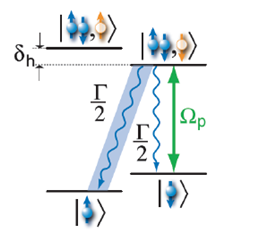
\includegraphics[scale=1]{ElectronEnergyDiagram}
  \caption{Electron Spin State diagram. A continuous wave laser drives this $|\downarrow \rangle \longleftrightarrow |\downarrow \uparrow,\downarrow \rangle$ spin state transition with rate $\Omega_{p}$. The excited state has a decay rate of $\Gamma $/2. $\Omega_{eff}$  is the effective transition rate between the spin-up and spin-down states, caused by the pulse sequence \cite{Nuclear_Feedback}.}
  \label{fig:ElectronEnergy}
\end{figure}

In this spin state diagram, an initial “optical pumping pulse” from a diode laser is applied to the electron. This repeatedly excites the population out of the spin-down state, $|\downarrow\rangle$, until there is a high probability that the electron is in the spin-up state, $|\uparrow\rangle$, which forms the initial state of the qubit. The electron will then receive the main pulse sequence of interest which will indirectly drive transitions between the spin-up and spin-down spin states. Finally, another pulse from the diode laser is applied to reinitialize the spin to the spin-up state. In this case, if the qubit has changed to the spin-down state during the experiment, it will emit a single photon which is measured with a single-photon counter. Therefore it is possible to determine the probability of being in the spin-up or spin-down state over many trials, which provides information on the coherence of the qubit system.


In a recent experiment involving dynamical decoupling at Stanford University, the researchers used two different lasers. One was a tunable-wavelength Titanium-Sapphire or Ti:Sapph pulsed laser and a 920-nm continuous-wave diode laser. The manipulation of the spin was achieved with various “rotation” pulses. These rotation pulses were created by the Ti:Sapph laser, which was mode-locked so that it output a pulse every 13 nanoseconds, with a pulse width on the order of picoseconds. By attenuating these pulses, they were able to create pulses which rotated the spin state by either 90 degrees or 180 degrees. These pulses are known as  $\pi$/2 and $\pi$, respectively because of the amount they rotated the spin state by \cite{Nuclear_Feedback}. After the Ti:Sapph laser rotates the electron spin thus changing the spin state, the diode laser rotates the electron to the spin-up state and stimulates photon emission that indicates the state of the spin at the end of the pulse sequence. 


\subsection{The Hahn Spin-Echo Sequence}
Some pulse sequences, like the Hahn spin-echo pulse sequence, have already been proven successful at increasing the decoherence time. Figure \ref{fig:Hahn} shows step-by-step how the spin orientation reacts to this series of pulses in a general Hahn spin-echo type sequence which is composed of a ($\pi$/2- $\pi$ - $\pi$/2) pulse train. While Figure \ref{fig:Hahn} is a good representation of what happens to the spin of the quantum dot system, it is important to note than in the quantum dot system for which the team is designing, it is the amplitude and not the duration of the pulses that is being varied to produce the $\pi$/2 and $\pi$ pulses. One other important difference is that a final $\pi$/2 pulse is used at the time of the echo to read the spin orientation in the quantum dot system.

In general, the Hahn spin-echo sequence begins with a $\pi$/2 rotation from the up state (Figure \ref{fig:Hahn}.B), after which the spin begins rotating in the magnetic fields. The spin is allowed to dephase for some time T(Figure \ref{fig:Hahn}.C), and then a $\pi$ pulse is applied to flip the spin (Figure \ref{fig:Hahn}.D). The principle of the sequence is that the effects of slowly varying background fields that accumulate before the $\pi$ pulse will be largely undone by the reverse action on the flipped spin after the $\pi$ pulse. In other words, the initial $\pi$/2 and $\pi$ pulses produce a “spin-echo” of the of the original spin orientation at time T after the $\pi$ pulse. (Figure \ref{fig:Hahn}.F). At this time a second $\pi$/2 pulse is applied to read the coherence of the spin 
\cite{Hahn_Spin_Echo}.


\begin{figure}[H]
  \centering
    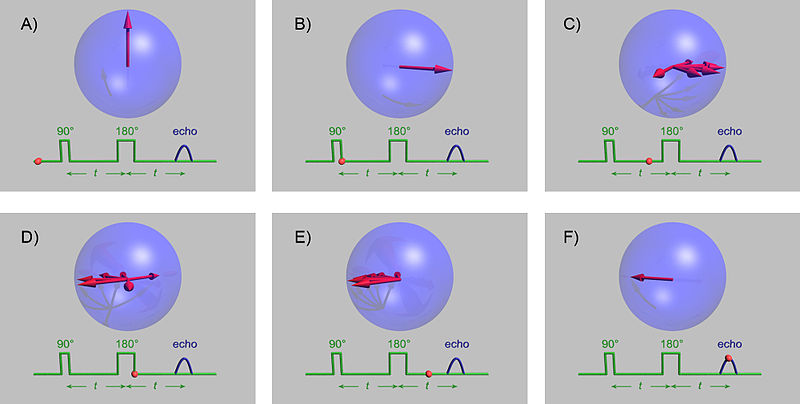
\includegraphics[scale=.450]{HahnSpinEcho}
  \caption{Hahn Spin-Echo Sequence. Frame A shows the average magnetic moment (red arrow) of a group of spins in their initial orientation. A $\pi$/2 pulse is applied in Frame B rotating the spins by 90 degrees. Frame C shows how the spins precess at different rates due to the flucations in the strength of the local magnetic field. A $\pi$ pulse is applied in Frame D, flipping the spins by 180 degrees. Frame E shows how the spins precess in the opposite direction until they refocus into an echo of the original spin state in Frame F. Note that for the quantum dot system, a final $\pi$/2 pulse is used at the time of the echo to measure that electron’s spin orientation. Also, the $\pi$ pulse is twice the amplitude of the $\pi/2$ pulse, rather than twice the duration \cite{spin_2014}.}
  \label{fig:Hahn}
\end{figure}

The experiment at Stanford University was published in 2010, and the authors report a decoherence time of 3 microseconds, three orders of magnitude improvement over the spin by itself. Figure \ref{fig:Stanford} shows a schematic of the optical network from Stanford University built to implement the Hahn Spin-Echo pulse sequence. The rotation laser output of regular pulses is sent first through a beam splitter, and then each of the two branches is passed through an electro-optic modulator (EOM). The EOMs can be controlled to either allow an individual pulse to pass or block it by rotating its polarization by 90 degrees. In this experimental setup, one EOM gates the top branch, which produces $\pi$/2 pulses, and another EOM gates the bottom branch, which produces $\pi$ pulses. The two branches are the same path length, apart from a small delay, $\tau$, in the $\pi$/2 branch. At the end of the experiment, the $\pi$ and $\pi$/2 pulses are recombined with a second beam splitter and coupled with the initialization pumping pulses from the diode laser\cite{de_greve_ultrafast_2011}.

\begin{figure}[H]
  \centering
    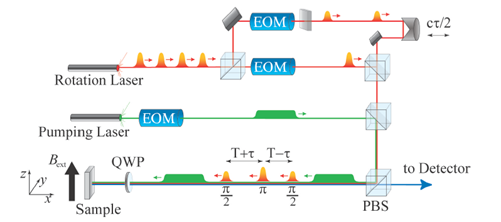
\includegraphics[scale=.75]{StanfordSetup}
  \caption{Experimental setup as used by the Yamamoto group at Stanford. The mode-locked rotation laser sends a series of pulses through a network of beam splitters and EOMs, producing the Hahn spin echo sequence \cite{de_greve_ultrafast_2011}.}
  \label{fig:Stanford}
\end{figure}

Although the diode laser is continuous wave, it is in series with an EOM that modulates its output to produce pulses of the appropriate intensity and repetition rate. The combined pulse sequence is then sent through a quarter wave plate in order to produce the correct polarization necessary to be accepted by the quantum dot sample. The experiments performed with this setup involved varying the delay of the $\pi$/2 pulses by extending the path length c$\tau$, as well as varying the separation, T, between $\pi$/2 and $\pi$ pulses by waiting longer before allowing a pulse from the Ti:Sapph laser through the EOMs (see Figure \ref{fig:Stanford}).These variations allow observation of the effect that the relative pulse timings have on the decoherence time\cite{de_greve_ultrafast_2011}.

While the optical setup described above has proven successful in controlling the electron spin with the implementation of the Hahn pulse sequence, other pulse sequences, such as ones with a greater number of pulses, may provide more precise control over the electron spin, increasing the decoherence time. While a system similar to the one from Figure \ref{fig:Stanford} might be designed to produce other sequences, the current reliance on expensive EOM optical components quickly makes cost, power, and space limiting issues. In order to increase the viability of spin control experiments for other pulse sequences, it is now necessary to create the sequences without the use of an unwieldy number of expensive, power-draining components.       

\subsection{The Uhrig Dynamical Decoupling Sequence}
\label{UDD}

The Uhrig dynamical decoupling (UDD) sequence is the first pulse sequence for which the team has been asked to create an optical network. The UDD sequence is a modification of a spin-echo sequence that theoretically extends the decoherence time of the electron spin qubit [3]. Like the Hahn spin-echo sequence, the same initial and final $\pi$/2 pulses are used to prepare the electron and check its state. However, between those $\pi$/2 pulses, the UDD sequence applies many $\pi$ pulses instead of just one. The key feature of the UDD sequence is that the spacing between each of the $\pi$ pulses is not constant, but follows a trigonometric progression as shown in Figure \ref{fig:timing} \cite{Uhrig}. Though such a sequence has theoretical support, it has not been experimentally verified thus far in this physical system. The Harvey Mudd clinic team is tasked with designing a network of optical components that will produce a UDD spin-echo pulse sequence for overall sequence lengths, $T$, between approximately 300 nanoseconds and 3 microseconds, and for between five and thirty $\pi$ pulses in the sequence.

\begin{figure}[H]
  \centering
    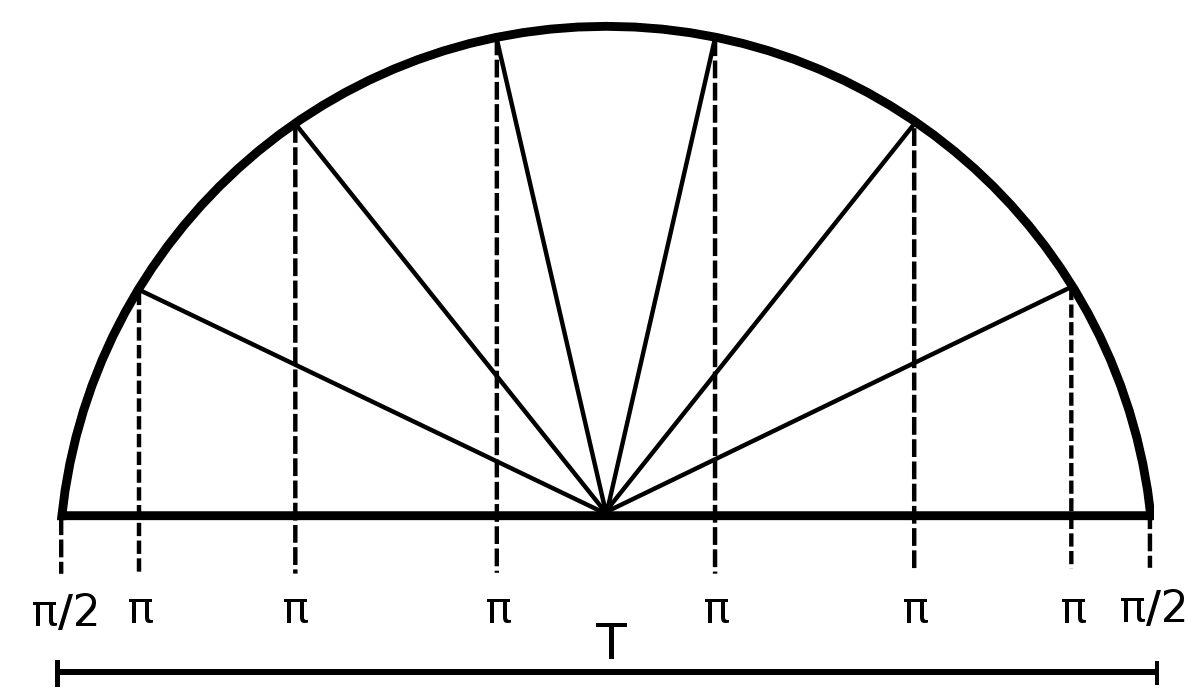
\includegraphics[width=.75\textwidth]{timing.png}
  \caption{This diagram shows the timings of the UDD sequence. The first and last vertical li	ne denotes the arrival of a $\pi$/2 pulse, and the remaining vertical lines denotes the arrival time of the $\pi$ pulses. The pulses are spaced according to the trigonometric function $t_j=T \sin^2\left(\frac{j \pi} {2N+2}\right)$ \cite{Uhrig}, where $T$ is the total sequence length, $N$ is the total number of $\pi$ pulses in the sequence, and $j$ is the index of a specific pulse in the sequence.}
  \label{fig:timing}
\end{figure}

There are a number of technical challenges that must be addressed in a satisfactory optical network design. First, the EOMs required for the nanosecond repetition rate are expensive elements; a feasible - and scalable - design would limit the number of costly components to two or three. Second, though the Ti:Sapph produces very powerful pulses, they are not infinite in energy. A suitable final design must still be able to create and apply $\pi$ and $\pi$/2 pulses, at the appropriate power levels, to the quantum dot. Third, there is limited space on the optical table. Taking into account the space required for the lasers and other overhead, about 4’ x 5’ of optical table remains.

With respect to the UDD sequence in particular, the variable spacing between pulses poses a major design problem. In the Hahn sequence, it was possible to use one branch of the network to create $\pi$ pulses and the other for $\pi$/2; that is not a feasible strategy for the UDD sequence. The separations between $\pi$ pulses are in general not multiples of the Ti:Sapph period, and because the timescales are too short for dynamic control of elements in the network, precisely replicating the UDD sequence requires a creative optical network design. Irregular delays between pulses pose a further difficulty to be addressed. However, the symmetry inherent in the sequence may allow for novel solutions. A system to generate arbitrarily-spaced pulses may not be feasible, but the structure of the UDD sequence does reduce the flexibility required of a full design.
    
A second task for the team to attempt is not a new pulse sequence in and of itself, but rather a modification of existing pulse sequences. Theoretical and experimental results indicate that splitting each $\pi$ pulse into two $\pi$/2 pulses and separating them by a fraction of the electron’s spin precession period improves the quality of the rotation\cite{soare_experimental_2014}. These sub-sequences within the overall sequence are known as compensation sequences. While constructing other optical networks, we should explore the possibility of integrating this feature into our designs.

\section{Optical Components}
The construction of one of these optical networks involves the incorporation and careful alignment of both static and dynamic optical components. While some of these components act passively, such as in the case of beam splitters, the development of these pulse sequences necessitates the use of dynamic electro-optic components in order to get the correct timing delays. The following section will focus on the physics behind the essential optical components used to build one of the optical networks, clarifying exactly how the pulses are modified by the system.

A variety of optical components are necessary to transform the initial input pulses into a final pulse sequence.The laser providing the initial input to the optical network is mode-locked, meaning it is providing a steady stream of laser pulses at a repetition rate of 13 nanoseconds. In order to produce a desired laser pulse sequence the optical network must delay, attenuate, and select the pulses from the steady stream of input pulses. To accomplish this transformation, polarization modulators in the form of Pockels Cells and polarizing beam splitters are used to choose between delays and select certain pulses for the sequence. Moreover, power attenuators such as electro-optic Modulators and beam splitters not only used to acquire a certain pulse power but, also to direct the pulses around the network.In conjunction, these optics modify the pulse sequence one step at a time until the desired sequence is produced.       

\subsection{Electro-Optic Modulators and Pockels Cells}

One of the key devices used in our design is an electro-optic modulator, or EOM, which can modify the amplitude, phase, or polarization of a laser pulse based on the voltage applied by a programmable driver. An EOM can essentially be broken down into two subcomponents: a linear polarizer and another interesting element known as a Pockels Cell which drives most of the pulse modifications \cite{RP_EOM}.

Pockels Cells are comprised of an electro-optic crystal, which has a refractive index dependent on the voltage difference across the crystal, which is applied via two electrodes. Since the amount of phase delay introduced into a light beam is dependent on the index of refraction of the medium it is propagating in, a Pockels Cell is most simply used as a pure phase modulator by varying the crystal's refractive index and aligning the beam along one of the crystal's optic axes to prevent changes in the polarization\cite{RP_Pockels_Cell}.      

Pockels Cells can also be used as a polarization modulators if one takes advantage of the crystal's birefringent properties. A material is birefringent when it has an index of refraction that is dependent on the polarization of the incident light. The birefringence of the electro-optic crystal is due to the existence of a fast and a slow optic axis within the crystal. The phase velocity of polarized light propagating through electro-optic crystal is dependent on its alignment with these axes. If the light is not completely aligned with one of these optic axes there will be a change in the phase velocity which changes its polarization \cite{RP_Birefringence}.

\begin{figure}[]
  \centering
    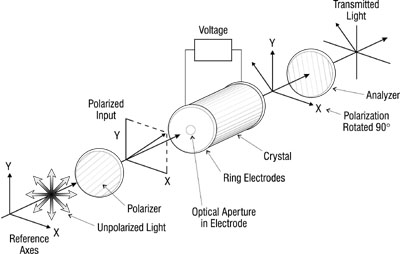
\includegraphics[scale=2.75]{PCschematic}
  \caption{Schematic of a Pockels cell with polarizers at each end. Polarized light is inputted into the Pockels cell, where its polarization is modified. The outgoing light will only be transmitted by the final polarizer if its polarization has been rotated 90 degrees from its initial state. Here the final polarizer is called an analyzer because it analyzes which polarization is transmitted\cite{simcik_module}.}
  \label{fig:PCschematic}
\end{figure}

Finally as shown in Figure \ref{fig:PCschematic}, we can easily obtain a change in the power by placing a polarizer at each end of the Pockels cell, effectively making it an EOM. A linear polarizer is an optical filter which only transmits light of a certain polarization. Therefore, in order to modify the power of an incoming light beam, we use the Pockels cell to modify its polarization and then use the polarizer to transmit only a certain polarization. In this way only a fraction of the power is transmitted\cite{RP_EOM}.     

\subsection{Important Specifications and Limitations}

There are a number of important specifications when choosing the best Pockels Cell for an experimental setup. Some significant factors of the experiment design that must be considered are the laser's repetition rate, the laser's beam size, the available voltage amplifiers, and the expected power density that the Pockels Cell will handle. All these factors will determine the Pockels Cell crystal type, electrode orientation, aperature size, and half-wave voltage.

Since a Pockels Cell is an electro-optic device, one of its more important properties is its half-wave voltage. The half-wave voltage is defined by minimum voltage required to induce a 180 degree phase change, which is also the same voltage required to go from minimum transmission to maximum transmission of the incident light\cite{RP_Pockels_Cell}. These voltages are usually on the order of a few kilovolts making use of a voltage amplifier in the experiment necessary. Since the half-wave voltage is a measure of the necessary electric field needed to change the properties of the Pockels Cell crystal, this voltage is dependent on the type of crystal used, aperature size, and the electrode orientation. For example, for transverse electrodes the half-wave voltage will be larger for greater aperature sizes since the electrode spacing will be larger. This larger spacing translates to a larger applied electric field and an increase in necessary voltage. On the other hand, for longitudinal electrodes the half-wave voltage is independent of the aperature size since a change in the aperature size doesn't change the electrode spacing \cite{RP_Pockels_Cell}.

Some of the most common crystal types used in Pockels Cells are Potassium Di-Deuterium Phosphate (DKDP) and $\beta$ -Barium Borate (BBO). While DKDP crystals are quite common and cost efficient, unfortunately they are not well suited for high-power and high repetition rate applications due to their relatively low repetition rate of a few kilohertz. On the other hand, BBO crystals have repetition rates on the order of  hundreds of kilohertz and they overall have a higher damage threshold than DKDP. BBO crystals also have a variable half-wave voltage since these crystals can be used with transverse electrodes. This means that for a given aperature size, the half-wave voltage may be lower for a BBO Pockels Cell than for a DKDP Pockels Cell\cite{United_Crystals}.

Ideally Pockels Cells would be able to change the phase, polarization, and power of a beam to whichever specifications is desired.  However, physical limitations, such as how quickly a programmable driver can apply a voltage change, will lead to non-ideal performance in the Pockels Cell. For example, Pockels Cells are unable to completely change the polarization of the incident light meaning that there will be residual light even at minimum transmission. The ratio of unwanted polarized light versus the amount of light with the desirable polarization at the maximum transmission is known as the contrast ratio and is a measure of a Pockels Cell’s efficiency as a polarizer. Similarly there exists an extinction ratio which characterizes a Pockels Cell’s efficiency at transmitting light at minimum transmission \cite{Sintec}. Lastly, when developing a design, the team needed to consider a Pockels Cell’s rise time which is a measure of how fast it can change from minimum to maximum transmission. The Pockels Cells considered in the current designs have a rise time of approximately eight nanoseconds meaning the pulses in the sequence must be separated by at least eight nanoseconds or else the Pockels Cell would be unable to properly modify the pulse \cite{Sintec}. All of these non-idealities will contribute to the error in the final pulse sequence. However, in an effort to characterize this error the team has included this non-ideal behavior in their Simulink simulations, further detailed in Section \ref{simulation}. 

\subsection{Polarizing Beam Splitters}

Another component integral to these optical networks is the polarizing beam splitter, which is used to select the desired pulses for the final pulse sequence. As its name implies, a regular beam splitter will split the power of an incident beam into two outgoing beams, usually at a 50/50 power ratio although other ratios can be produced. One of the most common non-polarizing beam splitter designs is a glass prism constructed out of two smaller triangular prisms that are epoxied together\cite{Properties_of_Prisms}. This design allows for a gap between the two triangular prisms which is essential for creating Frustrated Total Internal Reflection, the physical principle used to split the beams.

As light travels from one medium into another, it will be partially reflected and transmitted. However, at a certain angle of incidence known as the critical angle, the light will be totally reflected off a medium with a lower index of refraction. This phenomenon is known as Total Internal Reflection (TIR) and has many useful applications, most notably in the transmission of information through fiber optic cables. Even in TIR, there exists a residual or ``evanescent" wave that penetrates into the second medium. Although this evanescent wave only has a penetration depth of a few wavelengths, if yet another medium is introduced within a few wavelengths of the first medium one would observe the evanescent wave continue to travel into the third medium. This effect is known as Frustrated Total Internal Reflection (FTIR) and is analogous to the quantum tunneling effect in quantum mechanics. However, instead of having electrons tunnel through a energy potential barrier, here we have photons tunneling through a physical barrier\cite{FTIR}. 

\begin{figure}[h]
  \centering
    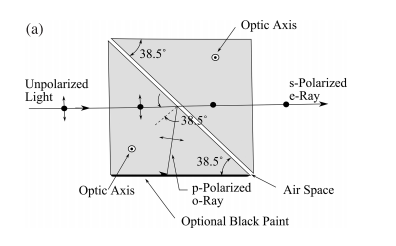
\includegraphics[scale=1]{GlanFoucaultPrism}
  \caption{Example of a Glan-Foucault polarizing beam splitter\cite{Properties_of_Prisms}.}
  \label{fig:GFPrism}
\end{figure}

In order to split a beam, we use FTIR at the air gap between the two triangular glass prisms of a cubic beam splitter. One of the outgoing beams produced is created by the TIR at the glass-air interface while the second outgoing beam is the transmitted beam due to effects of FTIR. Different splitting ratios can be obtained by changing the thickness of the air gap since the amount of energy transmitted by the evanescent wave into the glass prism is dependent on this distance \cite{Properties_of_Prisms}. 

Polarizing beam splitters can be created by using birefringent crystals, such as Calcite, for the prism material. The light incident on the beam splitter can be split along its polarization by using the fact that index of refraction is polarization dependent for these materials. One of most common polarizing beam splitters designs is known as the Glan-Foucault prism, which consists of two calcite prisms separated by an air-gap as shown in Figure. In Calcite, the index of refraction for the ordinary ray with p-polarization is 1.6557 while the index of refraction for the extraordinary ray with s-polarization is closer to 1.4852 for 630 nm light. This corresponds with a critical angle of 37.16 and 42.32 degrees for the p-polarized and s-polarized light respectively \cite{Properties_of_Prisms}. Therefore we can separate the light based on its polarization by choosing an angle of incidence that exceed the critical angle for one polarization but not the other. In this case, for the Glan-Foucault beam splitter, the p-polarization is separated using TIR while the s-polarization is transmitted through the air gap \cite{Properties_of_Prisms}. Note that imperfections in the birefringent prism and in the air gap will lead to non-ideal performance. One factor the team is taking into account is an imperfect splitting ratio, meaning that a 50/50 beam splitter may have a ratio closer to 51/49 or worse leading to error in the final pulse sequence.

\section{Computational Tools}
\label{sec:results}
The team has written a variety of computational tools to aid in analysis and simulation of the designs. A discussion of these tools, their preliminary results, and the effect these results have on the project is presented in this section.

\subsection{Optical Network Simulation}
\label{simulation}

Since these optical networks are difficult to create and test experimentally, simulation tools which accurately model reality are key for initially testing designs. In order to model each design, MATLAB's Simulink software was used. In Simulink, a library of modules for each optical component was created. These modules were then strung together in Simulink to create a computational model whose layout mimicked a potential optical table layout as shown in Figure \ref{fig:digitizing}. In order to model the optical network, the input pulse sequence is computed as a series of square wave pulses with a period corresponding to the repetition rate of the rotation laser of 13 ns. The code keeps track of the polarization amplitude of the light as a function of time throughout the optical network. The time steps used by the model are discretized in increments of 12.5 ps, which is much smaller than the 13 ns time between laser pulses. A list containing three vectors, a time vector, a vertical polarization amplitude vector and a horizontal polarization amplitude vector, is then passed into the Simulink model. The input vector is computed by rounding each pulse from the rotation laser to the nearest element in the time vector determined by the sampling frequency. All corresponding times in the Simulink model are computed relative to the closest element in this time vector. To better visualize pulses in the output plots, and to prevent longer computation times, the modeled pulse widths of the rotation laser were set to 50 ps in the model. Since the actual pulse width of the rotation laser that will be used in the experimental setup is 3-4 ps, the resolution of simulation will be increased in the future now that working optical network simulations have been successfully created.

Once the input sequence is determined, each Simulink module corresponding to an optical component modifies the input vector. The following optical components are currently modeled in the Simulink model: Pockels Cell, polarizing beam splitter, beam splitter, half-wave plate, linear polarizer, retroreflector, neutral-density filter, and a delay module for optical path lengths. Most of these modules modify the input vector in predicable ways. The polarizing beam splitter creates two output vectors of the appropriate single polarization to follow different paths in the model and the beam splitter module equally splits the input vector into two output vectors with the amplitude reduced by a factor of two. Besides the Pockels Cell, the remaining optical components are treated as ideal in the simulation. In Section \ref{sec:simadvance} the need to add inefficiencies to these components is addressed.

Each of these Simulink modules form an optical component library in Simulink shown in Figure \ref{fig:componentLibrary}. Individual modules can then be dragged into Simulink's model window, and combined to form an optical network as shown in Figure \ref{fig:simulink}. Notice the input and output ports of each module. These inputs consist of the input pulse, and  additional parameters which control how the module modifies the input pulse. For example, the beam splitter module takes three inputs, the input pulse, a transmit percentage, and an optional second input pulse. After correspondingly modifying the input pulse(s), the beam splitter outputs a transmitted and reflected pulse which can now be sent to different locations in the network. The optical network in Figure \ref{fig:simulink} is a model representation of Figure \ref{fig:digitizing}. Once provided with an initial pulse sequence, Simulink evaluates the optical network in Figure \ref{fig:simulink} by passing the input pulse in order through each module, evaluating how the module modifies the input pulse, and then sending the output pulse to the next module. Each component in Figure \ref{fig:simulink} is connected by ``wires'' which represent the flow of information in the model.  


\begin{figure}[H]
  \centering
    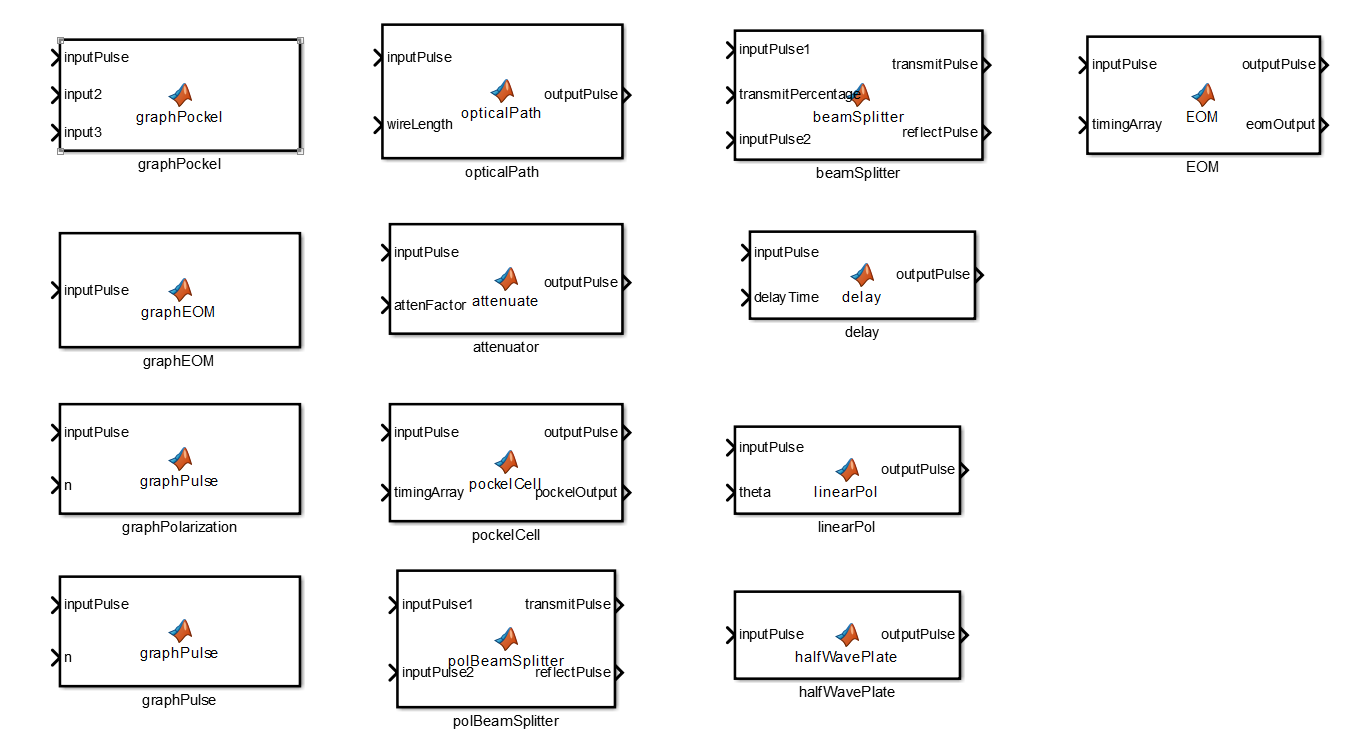
\includegraphics[width=0.9\textwidth]{OpticalComponentLibrary.PNG}
  \caption{The optical component library in Simulink containing the modules used to model optical networks such as in Figure \ref{fig:simulink}.}
  \label{fig:componentLibrary}
\end{figure}

\begin{figure}[H]
  \centering
    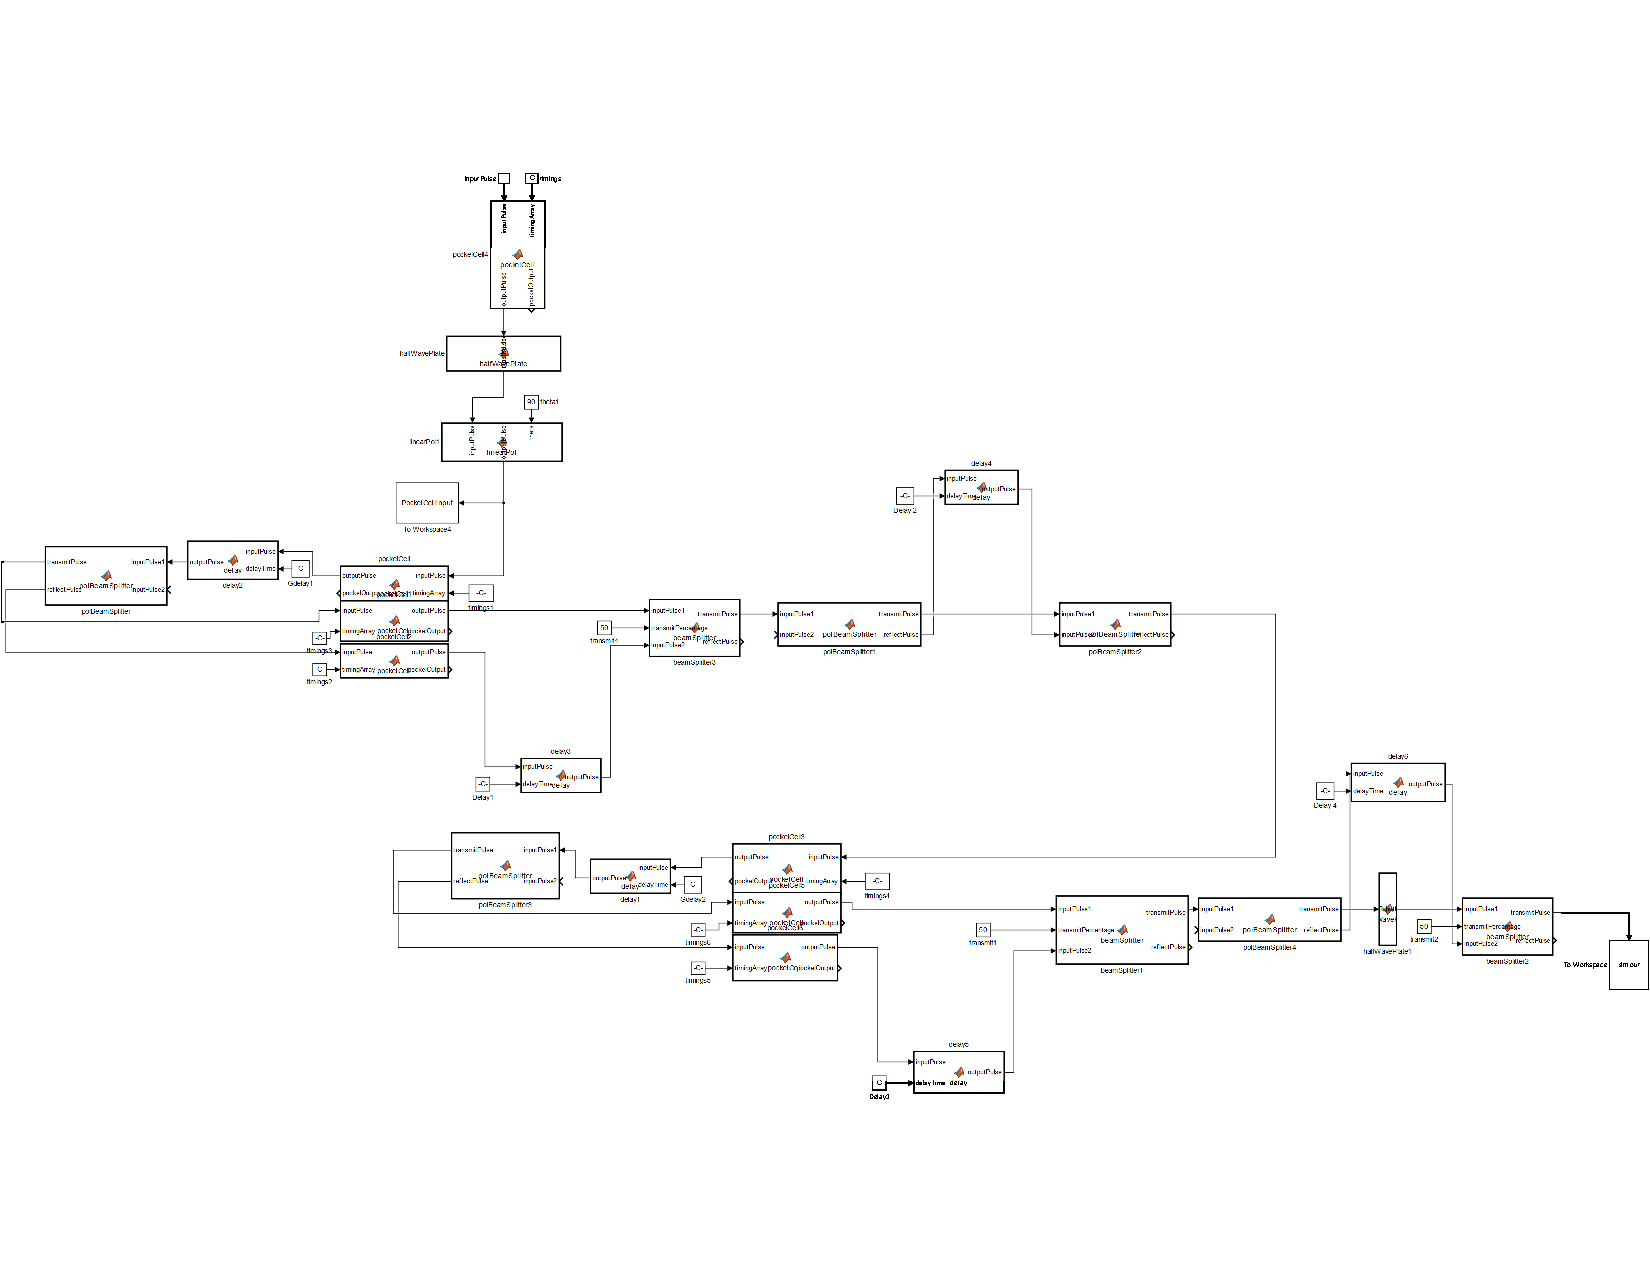
\includegraphics[scale=0.8, angle=90]{Digitizing_2Pi.pdf}
  \caption{Note that this image has been rotated counter-clockwise. The Simulink model created by connecting the modules in Figure \ref{fig:componentLibrary}. This model was used to test the optical network described in the detailed design section (see Figure \ref{fig:digitizing}).}
  \label{fig:simulink}
\end{figure}

In order to model inefficiencies associated with the Pockels Cells, Pockels Cell transmission curves such as Figure \ref{fig:bergmann} were used for inspiration. This transmission curve was used to represent the Pockel Cell in the figures in the detailed design section (see Figure \ref{fig:pulse5_A}). This transmission curve represents the optical transmission through the Pockels Cell and a following linear polarizer as a function of time. Input pulses which do not occur in the center of the transmission curve are not fully rotated, and are partially blocked by the following linear polarizer, resulting in reduced transmission. Since Pockels Cells have a characteristic rise and fall time, this curve models how long it takes for the Pockels Cell to fully rotate and transmit the pulse. Each input pulse which needs to be either fully rotated by the Pockels Cell or transmitted by a Pockels Cell-linear polarizer pair needs to occur in the center of the Pockels Cell transmission curve. The model Pockels Cell has a rise and fall time of 4 ns as shown in Figure \ref{fig:bergmann}. As mentioned previously, Pockels Cells typically have rise and fall times on the order of 8 ns. In this case, 4 ns was chosen to best model the rise and fall time of a potential Pockels Cell the team is considering using for the final design \cite{lightgate_pockel}. To determine the Pockels Cell control signal with a rise and fall time of 4 ns, the ideal delays were computed (see Section \ref{sec:optimizing}). Once the ideal times are known, the times each Pockels Cell should be rotating pulses can be calculated. A list of the times each Pockels Cell should be on is passed as an input parameter to the Pockels Cell modules in the Simulink model. Using the rise and fall times mentioned previously, the Pockels Cell module then computes a transmission curve centered on each of these input times.

\begin{figure}[H]
  \centering
    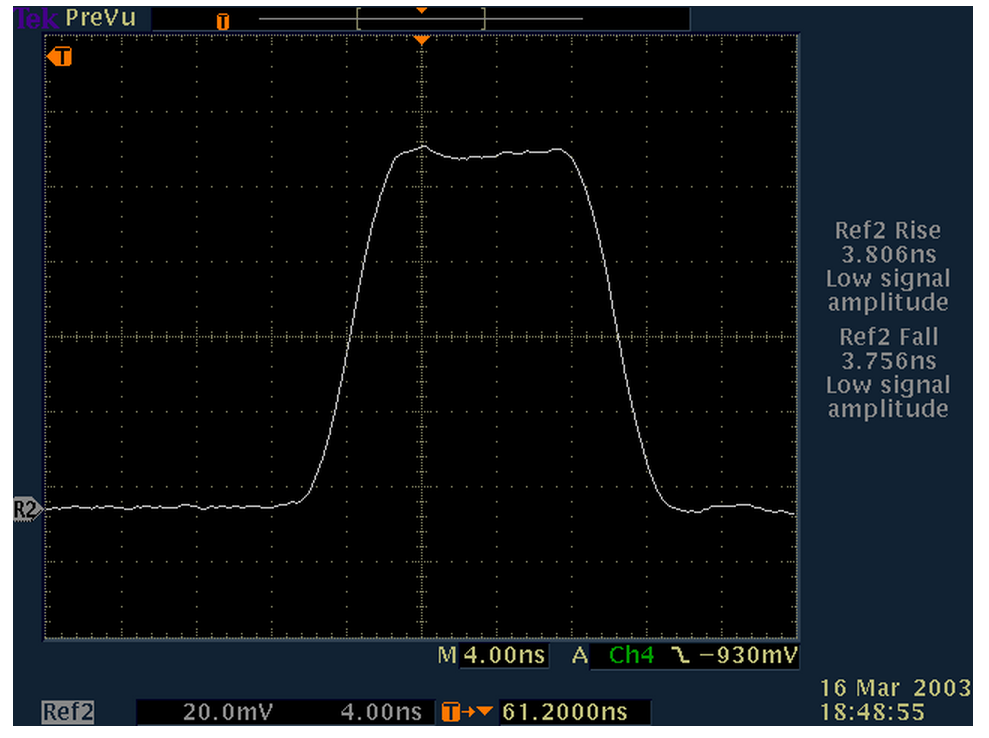
\includegraphics[scale=0.8]{BergmannPC.PNG}
  \caption{An example Pockels Cell transmission curve from Reference \cite{bme_pockel}.}
  \label{fig:bergmann}
\end{figure}

Further modeled Pockels Cell inefficiencies include a characteristic insertion loss and contrast ratio. Each of these parameters were obtained from a Gooch and Housego spreadsheet on the Lightgate series of Pockels Cells \cite{lightgate_pockel}. The insertion loss of 1.5\% attenuated the input pulse each time a pulse was sent through the Pockels Cell. Lastly, the contrast ratio determined which fraction of the input pulse was actually rotated to the opposite polarization. For the modeled Pockels Cell, the contrast ratio was 1000:1  \cite{lightgate_pockel}. For each input pulse, a fraction of 1000/1001 was successfully rotated, while a residual 1/1001 fraction of the input pulse was not rotated. These residual pulses then remained in the Simulink model, and were visible as having amplitudes on the order of 10$^{-4}$ as shown in the detailed design section. Currently the final amplitude of the pulses which will be delivered to the quantum dot is slightly less than 1/8 (0.1157) of the original amplitude, and the largest residual pulses are at amplitudes of $1.157 \times 10^{-4}$, a factor $10^{-3}$ below the output pulse. 

The Simulink model can also serve as an optical network debugging tool. In addition to optical components, plotting modules were added to the optical component library. These programs allow the current pulse train to be plotted after each stage in the model. These tools will be used to compare against physical testing results in the spring. To improve future comparisons with physical design testing, additional computation tools need to be developed to quantitatively compare the Simulink model's output sequence with the computed ideal pulses. 


\subsection{Delay Optimization}
\label{sec:optimizing}

Throughout the project, the team has written MATLAB code to aid in designing the optical network and evaluating its performance. As discussed in Section \ref{sec:detailed_design}, the current design includes several different delay paths that can be made adjustable by mounting the reflective optics on translation stages. If the optical network were intended to handle completely random pulse arrival times, then a set of delays that are evenly-spaced in time would be the optimal setup to minimize the digitization error. However, since $T$ and $n$ are fixed before an experiment is run, and therefore the ideal arrival times are fixed, the delays can be tuned to reduce the digitization error. Numerically, the optimization is accomplished by taking the pulse arrival times modulo 13 nanoseconds, and then minimizing the mean-squared error between ideal and digital pulse arrival times. An example of a successful optimization is shown in Figure \ref{fig:optimization_plot}. The set of possible delays is constrained in the optimization, however, as the composite delays are not independent. In the current design (Figure. \ref{fig:digitizing_pi2}), there are five different delay paths in the optical network - Delays 1-4, as well as the offset between the $\pi$/2 pulses and the $\pi$ pulses. Delays 1-4 are permuted to generate up to sixteen unique composite delay paths, but four of them must be reserved for the $\pi$/2 pulse-generating branch. The design is therefore not as effective as sixteen independent delay paths (an unfeasible optical network), but optimization is still an improvement over evenly-spaced composite delays.

The optimization's effectiveness declines as $n$ increases (Figure \ref{fig:msd_vs_n}), since the ideal arrival times become more randomly distributed (on average) over the 13-ns modular interval. If the number of pulses in the sequence is fewer than the number of composite delays, the mean-squared error will be either zero or very small; hence, the mean-squared error of the tunable delays in Figure \ref{fig:msd_vs_n} approaches zero as $n$ approaches 6 (since the data were calculated for a network with six composite delays). If $n$ instead is made much larger than the number of composite delays, it becomes impossible to match the ideal pulses exactly, and the mean-squared error will approach an upper bound equal to that of the evenly-spaced composite delay model (red curve). For these cases of large $n$, it may be possible to find values of $T$ such that the ideal pulse arrival times, modulo 13 nanoseconds, are somewhat grouped together instead of randomly distributed; the digitization error will be reduced in such a case. Thus, part of the role of the optimization for large $n$ will be to determine favorable values of $T$.

The shape of the optimized mean-squared curves depends on the number of composite pulses in the design - more composite pulses means that the $x$-intercept of the curve moves right, and the upper bound decreases. Thus, these curves can be used to evaluate the effectiveness of different designs. Specifically, the team plans to compare the current design (twleve composite delays) with a reduced version, in which only one Pockels Cell is used for delay selection. This simplification would reduce the number of composite delays to three, but also reduce the number of Pockels Cells by one. Thus, a much more cost-effective design can be had by sacrificing precision. Quantitative data on the precision diffences (via mean-squared error) will allow the team to provide an informed cost-benefit analysis of several designs in the spring semester.

\begin{figure}[H]
\centering
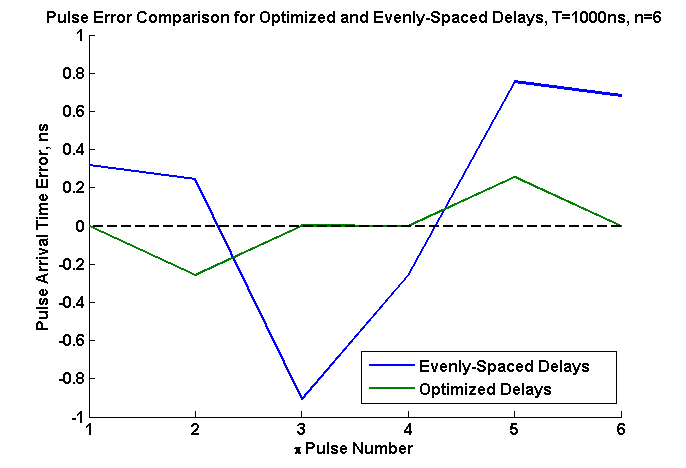
\includegraphics[width=0.7\linewidth]{delay_optimization_1us_n20.png}\caption{This plot is an example of a delay set optimization for $T=1000$ ns and $n=20$. The pulse arrival errors are plotted for both evenly-spaced and optimized delays. The optimization was performed with only three tunable delays (partially permuted to obtain six unique delay paths), but the optimization is able to achieve nearly-ideal pulses in the six-pulse sequence.}
\label{fig:optimization_plot}
\end{figure}

\begin{figure}[H]
\centering
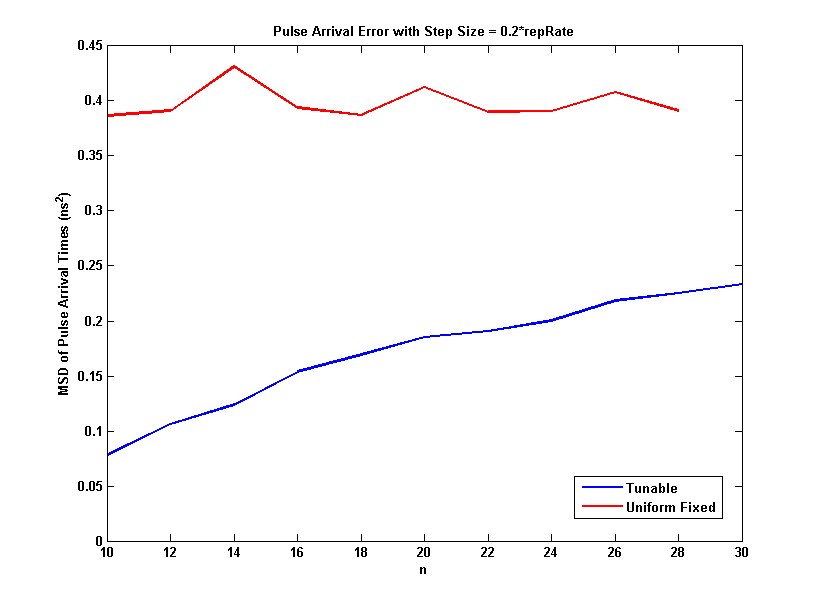
\includegraphics[width=0.7\linewidth]{msd_vs_n.png}\caption{Above, the mean-squared error, averaged over $T$ between 300 and 3000 ns, is plotted as a function of $n$. The network that was modeled for both curves has three delay paths (i.e. six composite delays). As expected, the error for the optimized delays tends toward zero as the number of pulses approaches the number of composite delays, and tends toward the upper bound of the evenly-spaced composite delays as $n$ becomes large.}
\label{fig:msd_vs_n}
\end{figure}

\subsection{Filter Function and Error Analysis}
\label{sec:error}
 Another important tool is filter function analysis, which is used for design validation. 
The pulse sequences produced by the digitizing design are not perfect. While these imperfections can be measured purely based on the differences between ideal and actual times, it is important to consider the larger picture. The point of the sequences is to minimize the effects of noise in the magnetic field surrounding the quantum dot, thus preserving the quantum information for longer. As such, the team can gain a better idea of how effective an imperfect sequence is by examining its effect on noise using a filter function\cite{ball_walsh-synthesized_2014}. 


The filter function is a measure of to what level the pulse sequence suppresses noise of angular frequency $\omega$. For values of $\omega$ where the filter function $F$ is small, the noise is suppressed well. The filter function of a UDD sequence of $\pi$ pulses can be approximated by the following sum:
\[F(\omega T) = \left| 1 + (-1)^{n+1} e^{i\omega T} + 2\sum_{j=1}^n(-1)^j e^{i\delta_j\omega T}\cos(\omega \tau_\pi/2)\right|^2\]
where $\delta_j T$ is the time of the $j$th $\pi$ pulse and $T$ is the total length of the sequence\cite{biercuk_optimized_2009}. This is a function of $\omega T$ to generalize the filter function for sequences of any length. The cosine term has to do with the finite width of the pulses, with $\tau_\pi$ being the width of a pulse. The team has been assuming pulses are instantaneous, and thus approximating this factor as 1. 

Figure~\ref{fig:filter1} shows the filter function for UDD sequences with various levels of precision. The dark blue line on the right is the filter function of a perfect UDD sequence. The light blue, red, and green lines are for sequences with varying levels of random imprecision. The green line is the most precise, with the difference between each pulse's actual time and the ideal time on the order of $10^{-6}$ smaller than the sequence's total length. This would correspond to an error of no more than a few picoseconds for a typical sequence. The purple curve is the filter function of a 3 microsecond sequence produced by the digitizing design from Figure \ref{fig:digitizing}. This is not our current digitizing design, as the current design includes compensation sequences, which we have not yet implemented in the filter function. Thus, the sequences produced by our current design are expected to create filter functions better than those shown in Figure \ref{fig:filter1}. However, even the filter function from the older design shows performance somewhere between that of the picosecond precision green curve and the hundred-picosecond precision red curve. 
The precision of the digitizing design sequence is slightly worse than that of the red curve's sequence, so the fact that it preforms better suggests our optimization is working.

\begin{figure}[H]
  \centering
    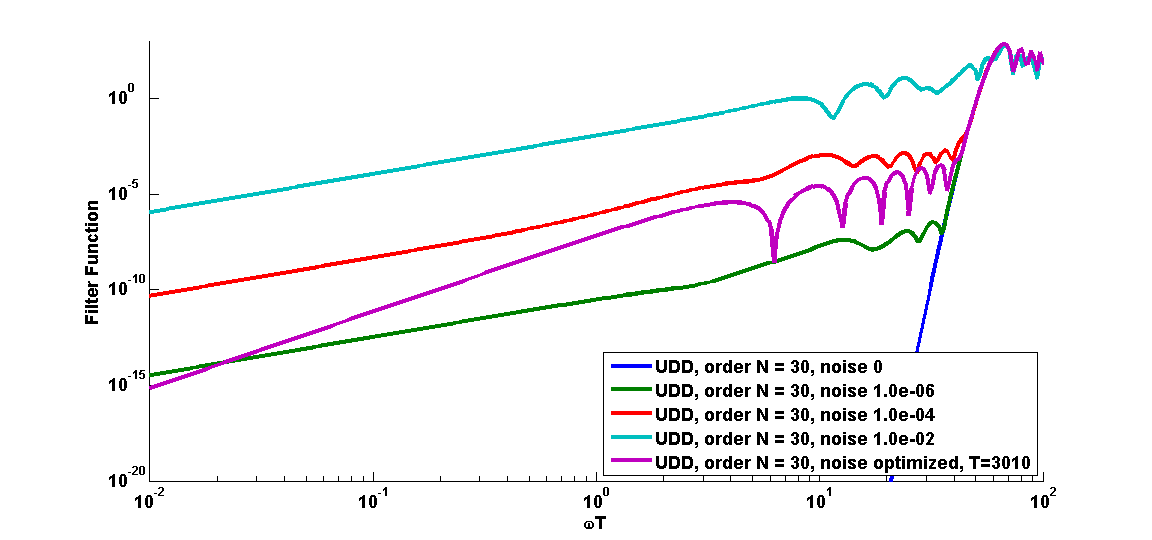
\includegraphics[width=\textwidth]{filter_opt_30_3010.png}
  \caption{Filter function for UDD sequences with various amounts of error. Filter functions represent the level to which noise is suppressed at different frequencies, so smaller values are better. The steep blue line on the right side represents the filter function of an ideal UDD sequence. The light blue, red, and green curves are the filter functions for sequences with varying levels of random error. The purple curve is the filter function for a sequence created by a digitizing design.}
  \label{fig:filter1}
\end{figure}

These filter functions provide a general idea of how well noise is reduced by a pulse sequence, but it is difficult to relate this to actual effectiveness. The true effectiveness of the filter function is only evident if it is integrated against the actual noise, but that is unknown according to the liaisons, so the filter functions must be judged by some of their other characteristics. For example, the slope of the function as $\omega T$ goes to small values, or its value for some specific $\omega T$ value could be used to measure its effectiveness. It is important to understand and measure the effectiveness of a sequence, as slight changes to a pulse sequence can drastically affect the shape of a filter function. In Figure \ref{fig:filter2}, the filter functions of many very similar pulse sequences are plotted. All the sequences had 16 pulses, and ranged in length from about 1.4 microseconds to about 1.7 microseconds. Despite the sequences all being similar, a great deal of variation is seen in the filter functions. At $\omega T=10^{-2}$, the values of the filter function range over four orders of magnitude.


\begin{figure}[H]
  \centering
    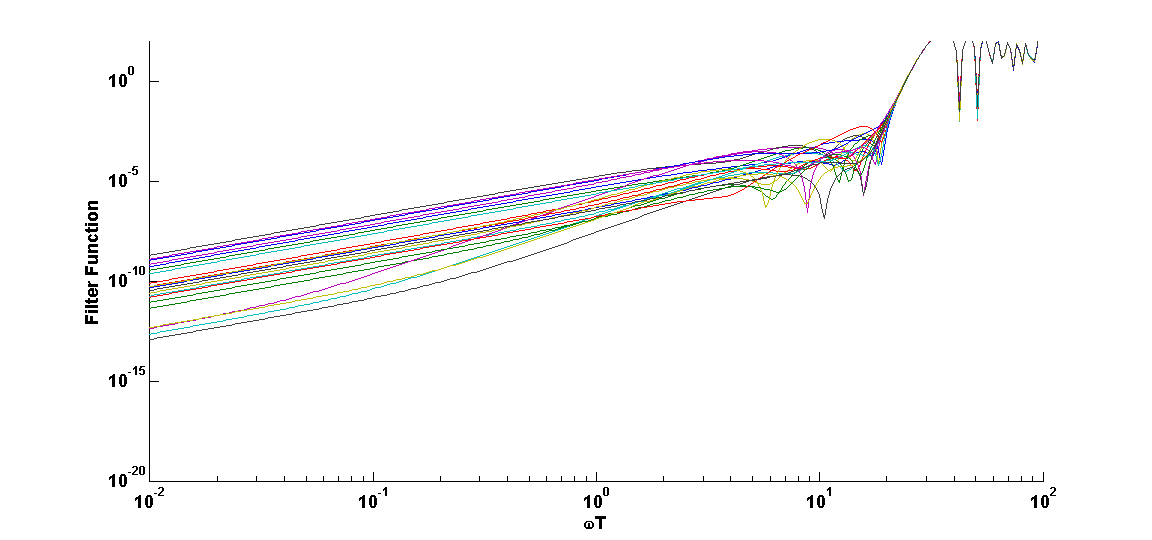
\includegraphics[width=\textwidth]{erroranalysis1.png}
  \caption{Filter functions derived from many similar sequences. Twenty UDD sequences, all with 16 pulses and lengths from 1.4 microseconds to 1.7 microseconds, were produced by a simulation of a digitizing design. Despite the similarity of the UDD sequences, the filter functions vary significantly.}
  \label{fig:filter2}
\end{figure}

The variation in filter functions is complicated by unclear relationships between the filter functions and pulse sequences. The digitizing designs introduce discretization error into the sequences, which can be measured in a few ways. The digitizing designs were first tuned to minimize the mean-squared-difference (MSD) between ideal and actual pulse timings. However, further investigation found that the MSD is not a good indicator of filter function effectiveness. Figure \ref{fig:filter3} shows a scatterplot of function filter effectiness, measured by the the filter function value at $\omega T = 10^{-2}$. This value gives an idea of how steep the rolloff of the filter function is, with smaller values indicating a steep rolloff and a better filter function. This value was plotted for the twenty filter functions shown in Figure \ref{fig:filter2} against both the MSD and the maximum difference between the actual and ideal timing of a pulse in each sequence. There is no clear correlation between either of these error measurements and the filter function's shape. Although the best filter functions had low MSD, many of the worse filter functions had MSD just as low or lower.

\begin{figure}[H]
  \centering
    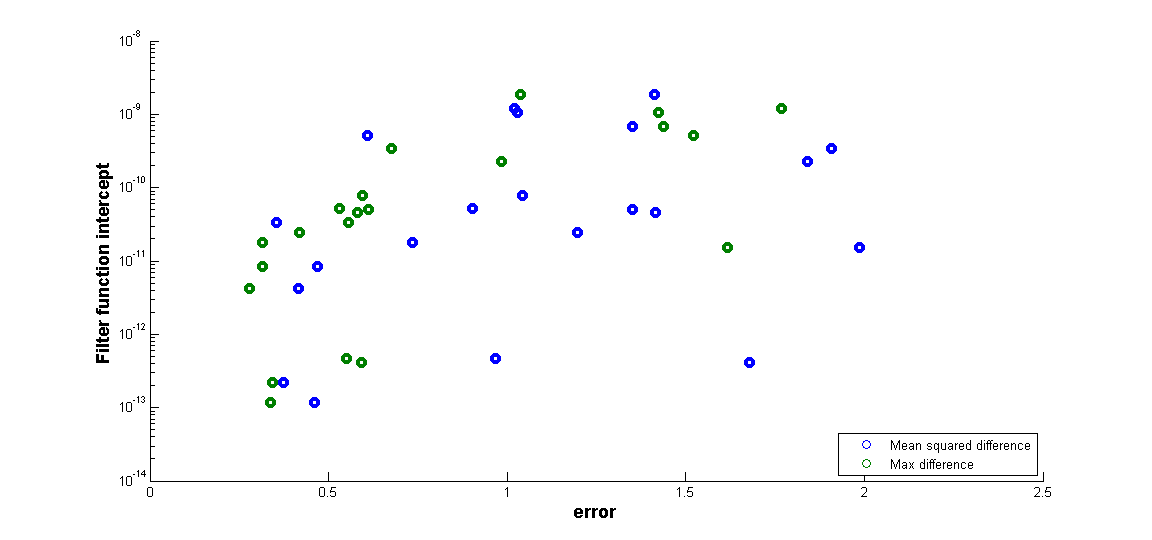
\includegraphics[width=\textwidth]{erroranalysis2.png}
  \caption{Filter function values at $\omega T=10^{-2}$ plotted against the error in the pulse sequences. The effectiveness of the filter functions in Figure \ref{fig:filter2} are compared to the error present in the pulse sequence timings used to generate the filter functions. Error is measured as mean-squared-difference (MSD) between actual and ideal pulse timings and as the maximum difference between actual and ideal pulse timings.}
  \label{fig:filter3}
\end{figure}

However, insights into how the UDD sequence works have suggested other characteristics to investigate. As each $\pi$ pulse in a UUD sequence switches the direction of precession of the electron's spin, a switching sequence, where the value switches from 1 to -1 or vice versa at each pulse timing, could represent how the spin precesses\cite{west_near-optimal_2010}. Integrating this switching sequence should measure how much the spin precesses beyond what is ideal, and thus give an indicator of the sequence's effectiveness. 


These insights into investigating error and filter functions suggest a few action items to complete next. As the integral of the switching sequence is equivalent to the sum of the timing errors with alternating signs, the team should verify that such an alternating sum is a good metric for filter function performance by taking the filter functions graphed in Figure \ref{fig:filter2} and plotting the value at $\omega T = 10^{-2}$ against the sum of time errors. If the sum of time errors is verified to indicate filter function performance, the optimization code mentioned in Section \ref{sec:optimizing} should be rewritten and re-tested to minimize that instead of MSD. Other places where MSD was used, such as in Figure \ref{fig:msd_vs_n} could also be redone with sum of timing errors in place of MSD. In addition, the team will remake the performance graph of Figure \ref{fig:msd_vs_n} for the full range of pulse sequences $n=1$ to $n=30$, and for a range of different digitizing designs.  This analysis will help clarify the tradeoff between equipment budget and pulse sequence performance.

\section{Design Evaluation}
\label{sec:design_evaluation}

\section{Single Pulse Design}
\label{sec:single_pulse_design}
Single-pulse designs are characterized by using only a single pulse as the input to the optical network. An initial EOM will select a single pulse, which will then be split up into multiple pulses by beam splitters. These pulses will travel along different optical paths, encountering different delays and undergoing different attenuations. All the pulses will eventually be redirected onto a single path to produce the final output pulse sequence. 

\subsection{Specific Design (TODO Rename this subsection)}
As all output pulse are derived from a single pulse, the time delay between the pulses must be produced by time-of-flight delays on the optical table. Recognizing that the table space needed to produce these delays would be the primary fault of this type of design, we created a design that would minimize the delays needed by utilizing the symmetry of the UDD sequence to reuse delays. This single-pulse design, for a sequence of six $\pi$- pulses and two $\pi/2$-pulses, is shown in Figure~\ref{fig:singlepulse}. 

\begin{figure}[t]
\centering
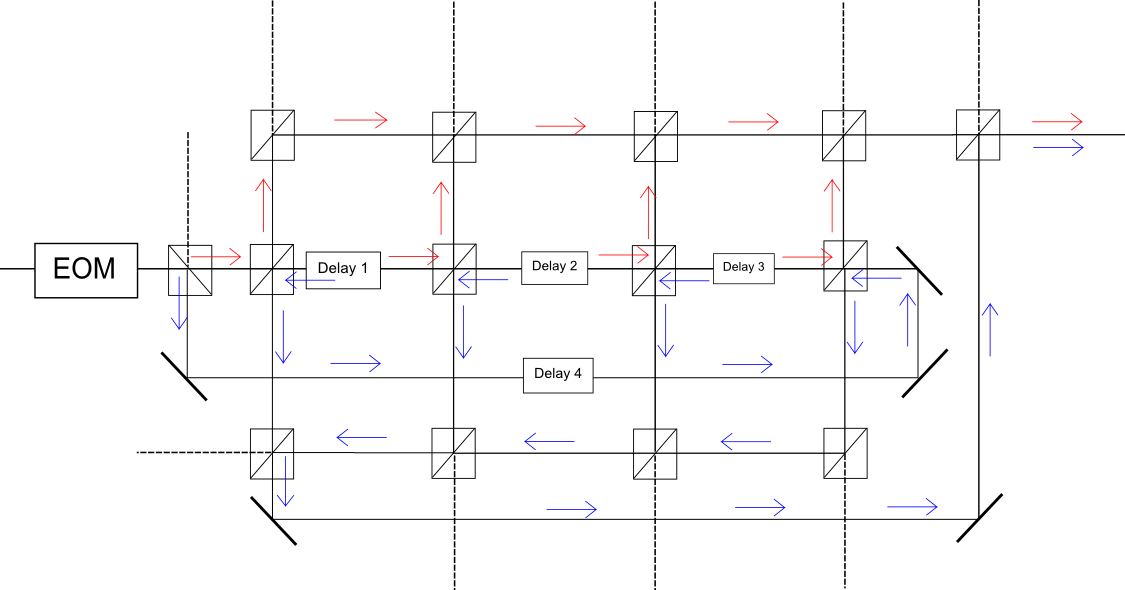
\includegraphics[width=\textwidth]{singlepulse.png}
\caption{Example of single-pulse design. The EOM lets in a single pulse, which is split into many pulses by the numerous beamsplitters.}
\label{fig:singlepulse}
\end{figure}

In this design, a single pulse enters through the EOM on the left, is split across four paths of different delays, and is recombined on the right. The first beamsplitter splits the pulse along two paths, denoted by red and blue. The red path creates the first half of the sequence, while the blue path creates the second half. Following the leftmost red arrow, we see that the pulse hits another beamsplitter, directing one pulse upward and another pulse forward. The upward-heading pulse is sent into the upper recombination path, and will continue until it exits the system on the right. As it has received no explicit delay, it will be the first $pi/2$-pulse, starting the sequence. Meanwhile, the pulse that was transmitted through the beamsplitter will enter delay 1. In the diagram, this and all other delays are abstracted as generic delays, as depending on their length, the delay could be provided by retroreflectors or Harriott cells. Delay 1 will delay the pulse by a time equal to the time between the first $\pi/2$-pulse and the first $\pi$-pulse of the UDD sequence. The delay times are illustrated in Figure~\ref{fig:UDDseqdelays}. After being delayed, the pulse is sent through another beamsplitter, where the reflected pulse is sent to the recombination line to become the first $\pi$-pulse and the transmitted pulse is sent onwards to go through additional delays and beamsplitters to become the rest of the $\pi$-pulses in the first half of the sequence.

If we look back at the very first beamsplitter, we see the reflected pulse is sent along the blue path. The blue path includes delay 4, which is the longest delay in the design. It must be equal to the time between the first $\pi/2$-pulse and the first $\pi$-pulse of the second half of the sequence. It then passes through the line of delays and beamsplitters that the earlier pulses had, but in the opposite direction. This applies the delays in the opposite order in order to create the symmetrical UDD sequence. The beamsplitters reflect the pulses downwards, where they are combined in this reverse order before being combined with the red path pulses.

The total length of the labeled delays will be equal to the total length of the UDD sequence. Extra path length introduced by the physical setup of the design can either be dealt with by making sure extra path length is added symmetrically to each branch of the design or by decreasing the length of labeled delays by corresponding amounts.



\begin{figure}[H]
\centering
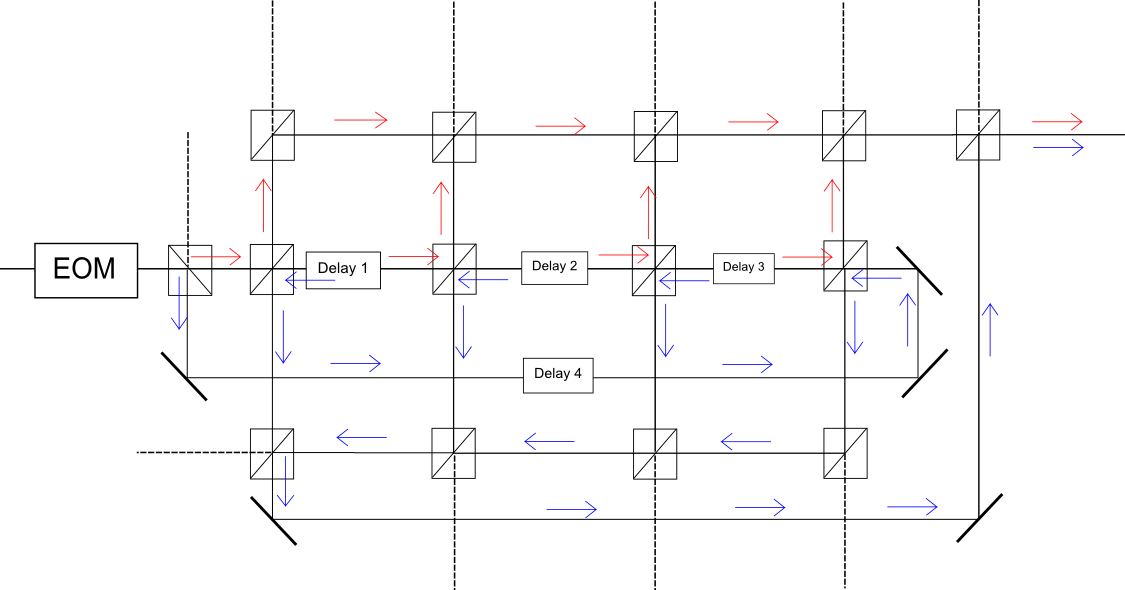
\includegraphics[width=\textwidth]{singlepulse.png}
\caption{TODO implement image of UDD sequence and how the delay lengths match up with the sequence times.}
\label{fig:UDDseqdelays}
\end{figure}

\subsection{Evaluation}

These designs have several advantages. They generally require only a single EOM, saving greatly on cost and optical table space. Because these designs only use a single pulse, they are not constrained by the pulse repetition rate of the mode-locked laser. And because all the output pulses are derived from a single pulse, it is easy to generate many pulses all closely spaced with each other. However, these designs also have significant drawbacks. While it is easy to generate closely spaced pulses with this type of design, generating distantly spaced pulses requires long delays that require more complex optics or consume large amounts of optical table space. If the total sequence length is over 100 nanoseconds, the delays required are in the tens of nanoseconds. As light travels about one foot in a nanosecond, optical paths of twenty or more feet in length would be required. 

Additional problems include power concerns. Every time a pulse is split, the resulting pulses have half the power of the initial pulse. Additionally, recombining the split pulses along a single path must be done with beamsplitters, losing additional power. Even the best design of this type, shown in Figure~\ref{fig:singlepulse}, has a power loss factor of $2^{-7}$ for an 8 pulse sequence. This means each output pulse will have $1/128$ of the power of the input pulse. For sequences with more pulses, this ratio would only get worse, as it scales by $2^{-3-n/2}$. Therefore, if many pulses are needed, there may be insufficient power to produce them all from the single pulse.






\section{Digitizing Designs}
\label{sec:digitizing_designs}
The other type of design has been termed “digitizing” designs. They are so named because instead of having a precisely tuned delay for each pulse, such that every pulse is output exactly where it is supposed to be in the sequence, a number of delays are shared between all pulses, such that only certain discretized pulse output times are possible. This results in discretization error, which reduces the effectiveness of the pulse sequence, but allows for greatly increased flexibility in the variety of sequences a single design can produce.

For example, the simplest digitizing design would be an EOM and nothing else. Although it would not be possible to produce an output pulse at the exact time desired, pulses would be arriving at the EOM every 13 nanoseconds, so by letting through the pulse nearest to the desired time, you would be guaranteed to produce a pulse within 6.5 nanoseconds (half of 13 nanoseconds) of the desired time. If you added to this an optional delay of 6.5 nanoseconds, you could produce output pulses at any integer multiple of 6.5 nanoseconds, increasing your precision. An example of a simple optional delay is shown in Figure ~\ref{fig:simple}. By adding successive smaller optional delays, you could further increase the precision until the sequence would be nearly as effective as one with the exactly desired pulses.
    
 \begin{figure}[t]
\centering
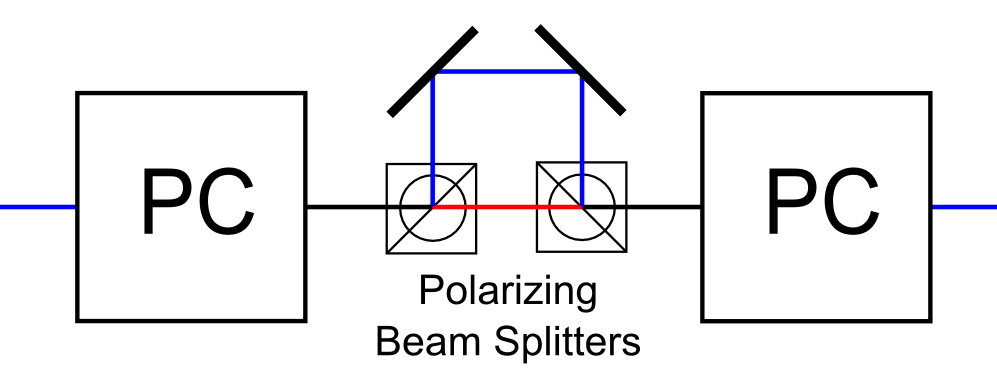
\includegraphics[width=0.8\textwidth]{simple_digitizing.png}
\caption{A simple example of a digitizing design. The initial Pockels Cell rotates the incoming pulse's polarization so that it either takes the short path or the long path through the polarizing beam splitters. The Pockels Cell on the right then rotates the pulse's polarization back to its original state, so that all output pulses have the same polarization. Thus, by controlling the Pockels Cells, the experimenter can choose to delay certain pulses while letting other pulses through undelayed.}
\label{fig:simple}
\end{figure}
    
Because the same collection of delays is used for each pulse in a sequence, this means a sequence can be extended indefinitely without having to change the design. A single design could create a 6-pulse sequence or a 30-pulse sequence. To optimize the precision of the pulse timings, it would be necessary to make slight changes to the delays between different sequences. However, these tunable delays would be simple to implement using retroreflectors on adjustable platforms. Digitizing designs are thus immensely flexible, as a single design could create almost any sequence. 
    
Of course, there are disadvantages to digitizing designs. There is a limitation on the type of sequence these designs can create. If the pulse are too closely spaced, problems may arise. For example, our current digitizing design, detailed in Section \ref{sec:detailed_design}, can only create sequences where the pulses are at least 20 nanoseconds apart. Another disadvantage is that the timings of the Pockels Cells become complex and tedious to ascertain by hand, so computer tools had to be developed to assist the timing management. Most importantly, the introduced discretization error decreases the effectiveness of the sequence, so evaluating and minimizing the error is an important consideration.

\subsection{Design Details}


 \begin{figure}[t]
\centering
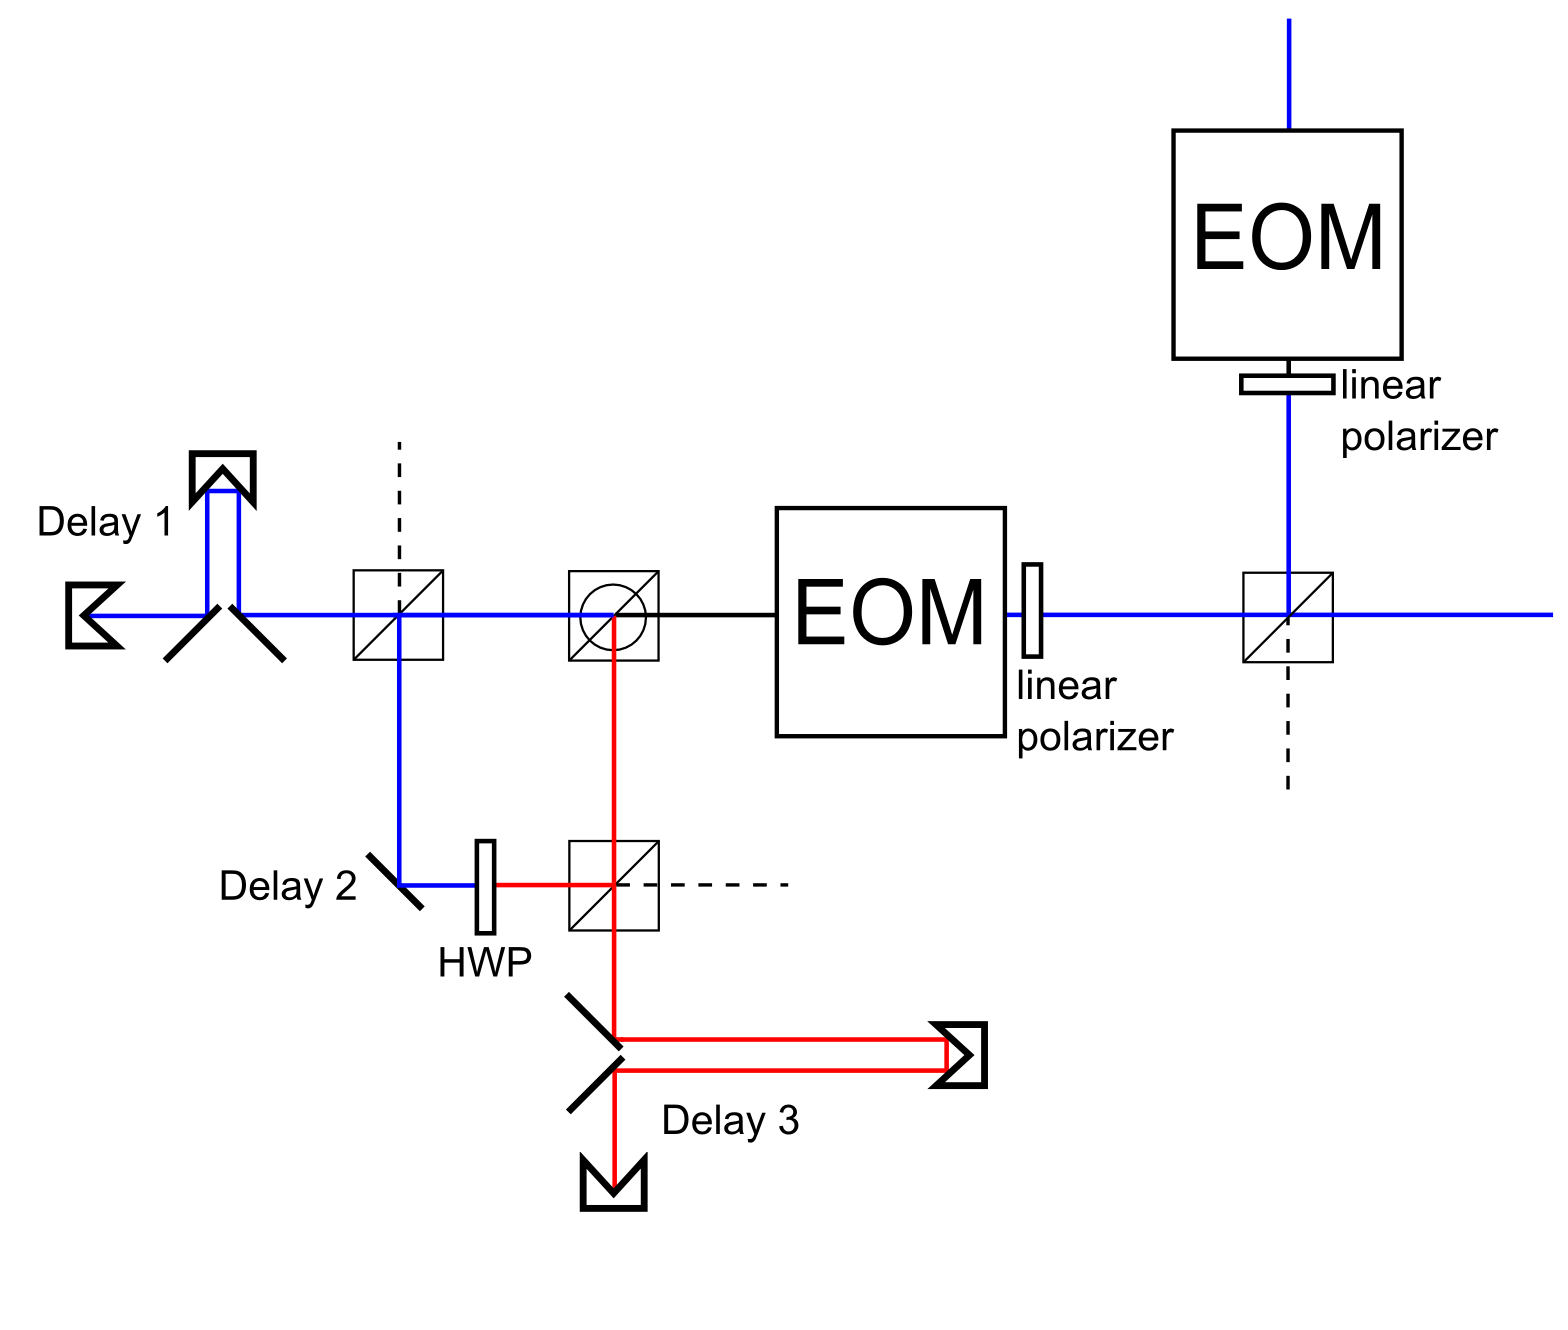
\includegraphics[width=0.8\textwidth]{digdesign1.png}
\caption{Caption goes here.}
\label{fig:digdesign1}
\end{figure}



\section{Design Summaries}
\label{sec:design_summary}

\section{Design Alternatives}
\label{sec:design_alternatives}
The team started by devising multiple design alternatives. As the project requires creating designs for a variety of laser pulse sequences, which may differ substantially in the timescales involved, the number of pulses used, and the types of pulses created, the team initially thought it would be necessary to create multiple optical networks in a variety of designs. However, after several iterations of designs had been considered, the possibility of using a single flexible design for many different laser pulse sequences appeared to be feasible. This section lists some designs the team considered, and provides a comparison of their qualities. The rejected alternatives may still provide useful insights for other designs even if they are not feasible for the current experiment parameters.

	The types of designs that were considered can be divided into three categories.  Path-per-pulse designs are characterized by having a separate path for each pulse or pair of pulses. Single-pulse designs create the full sequence from a single initial pulse which is split up and delayed across different paths to form the entire sequence. Digitizing designs are characterized by having a fixed number of different delays shared between all pulses, giving the design great but not total flexibility in the sequences that it can create.
    
\subsection{Path-per-Pulse Designs}
Path-per-path designs are characterized by having separate paths for each pulse. This design was considered first, due to its successful use in previous experiments. The design shown previously in Figure~\ref{fig:Stanford} was an example of this type of design, with two separate paths, each with its own EOM. Generally,  for each pulse or pair of pulses in the output sequence, there must be a corresponding branch in the network, with delays customized to that pulse. The specialization of each branch allows these designs to create complex output pulse sequences, but they have significant disadvantages. As each pulse in the sequence requires its own branch in the design, including an EOM, the cost of these designs quickly becomes prohibitive as the number of pulses in the sequence increases. It may be possible to use novel designs to fit a pair of pulses in a single branch or to otherwise use fewer EOMs, but even then, a large amount of optical hardware is still required, making it difficult to fit the design on the optical table. Therefore, the team quickly looked to other types of designs.

\subsection{Single-Pulse Designs}



\subsection{Digitizing Designs}
\label{sec:digitizingDesign}
The type of design on which the team is currently focusing have been termed “digitizing” designs. They are so named because instead of having a precisely tuned delay for each pulse, such that every pulse is output exactly where it is supposed to be in the sequence, a number of delays are shared between all pulses, such that only certain discretized pulse output times are possible. This results in discretization error, which reduces the effectiveness of the pulse sequence, but allows for greatly increased flexibility in the variety of sequences a single design can produce.

	For example, the simplest digitizing design would be an EOM and nothing else. Although it would not be possible to produce an output pulse at the exact time desired, pulses would be arriving at the Pockels Cell every 13 nanoseconds, so by letting through the pulse nearest to the desired time, you would be guaranteed to produce a pulse within 6.5 nanoseconds (half of 13 nanoseconds) of the desired time. If you added to this an optional delay after the Pockel Cell of 6.5 nanoseconds, you could produce output pulses at any integer multiple of 6.5 nanoseconds, increasing your precision. An example of a simple optional delay is shown in Figure ~\ref{fig:simple}. By adding successive smaller optional delays, you could further increase the precision until the sequence would be nearly as effective as one with the exactly desired pulses.
    
 \begin{figure}[t]
\centering
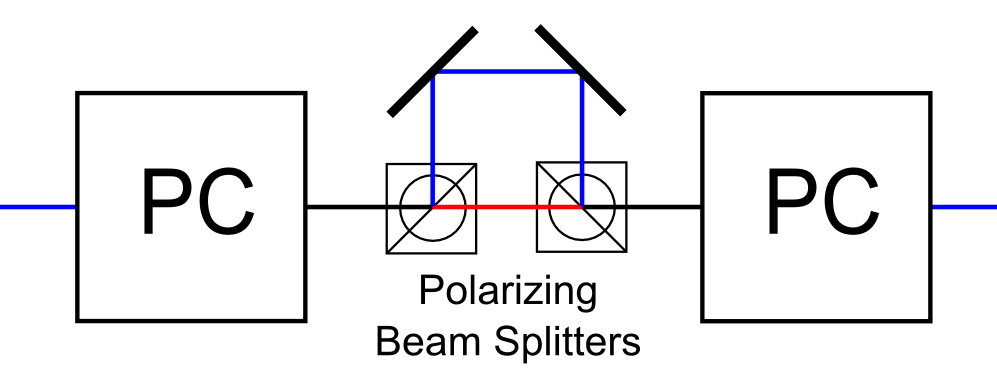
\includegraphics[width=0.8\textwidth]{simple_digitizing.png}
\caption{A simple example of a digitizing design. The initial Pockels Cell rotates the incoming pulse's polarization so that it either takes the short path or the long path through the polarizing beam splitters. The Pockels Cell on the right then rotates the pulse's polarization back to its original state, so that all output pulses have the same polarization. Thus, by controlling the Pockels Cells, the experimenter can choose to delay certain pulses while letting other pulses through undelayed.}
\label{fig:simple}
\end{figure}
    
	Because the same collection of delays is used for each pulse in a sequence, this means a sequence can be extended indefinitely without having to change the design. A single design could create a 6-pulse sequence or a 30-pulse sequence. To optimize the precision of the pulse timings, it would be necessary to make slight changes to the delays between different sequences. However, these tunable delays would be simple to implement using retroreflectors on adjustable platforms. Digitizing designs are thus immensely flexible, as a single design could create almost any sequence. 
    
Of course, there are disadvantages to digitizing designs. There is a limitation on the type of sequence these designs can create. If the pulse are too closely spaced, problems may arise. For example, our current digitizing design, detailed in Section \ref{sec:detailed_design}, can only create sequences where the pulses are at least 20 nanoseconds apart. Another disadvantage is that the timings of the Pockels Cells become complex and tedious to ascertain by hand, so computer tools had to be developed to assist the timing management. Most importantly, the introduced discretization error decreases the effectiveness of the sequence, so evaluating and minimizing the error is an important consideration.


\subsection{Design Alternatives Comparison}
\label{sec:comparison}

The three design alternatives all had various advantages and disadvantages, which are summarized in Table \ref{tab:compare}. Most notably, the designs differ in both effectiveness and cost-efficiency at different sequence lengths and number of pulses per sequence. While a path-per-pulse design can pick pulses at any time to produce a sequence of any length, adding more pulses to a sequence requires costly EOMs or Pockels Cells. For a single pulse design, physical space limitations put an upper limit to how long a pulse sequence can be, and power loss constrains how many pulses can be in a sequence. Digitizing designs have no real upper bound to sequence length, but are incapable of producing short sequences with many pulses. The desired pulse sequences have 10-30 pulses, and are 100-3000 nanoseconds in length, or possibly even longer. This makes digitizing designs the best option. Although digitizing designs are the most complex, both to construct and to understand, and also introduce discretization error into the sequences, leading to reduced precision, they are the only type of design capable of producing long sequences with many pulses.

\begin{table}[H]
\centering
\begin{tabular}{|l|c|c|c|}
\hline
\textbf{} & \multicolumn{1}{l|}{\textbf{Path-per-Pulse}} & \multicolumn{1}{l|}{\textbf{Single-Pulse}} & \multicolumn{1}{l|}{\textbf{Digitizing}} \\ \hline
\textbf{Simplicity} & $\star\star\star$ & $\star\star$ & $\star$ \\ \hline
\textbf{\begin{tabular}[c]{@{}l@{}}Effective Range\\ of Sequence Length\end{tabular}} & Any & \begin{tabular}[c]{@{}c@{}}\textless  $~100$ ns,\\ due to physical\\ constraints\end{tabular} & \begin{tabular}[c]{@{}c@{}}Long sequences,\\ such that pulses are\\ separated by \textgreater 20 ns\end{tabular}  \\ \hline
\textbf{\begin{tabular}[c]{@{}l@{}}Effective Range\\ of \# of Pulses\end{tabular}}  & \begin{tabular}[c]{@{}c@{}}\textless $~6$, \\ due to cost\end{tabular} & \begin{tabular}[c]{@{}c@{}}\textless $~10$,\\ due to power\\ loss constraints\end{tabular}     & \begin{tabular}[c]{@{}c@{}}Dependent on\\ sequence length\end{tabular} \\ \hline
\textbf{\begin{tabular}[c]{@{}l@{}}Pulse Timing\\ Precision\end{tabular}} & $\sim 1$ ps & $\sim 1$ ps & $\sim 500$ ps \\ \hline
\end{tabular}
\caption{Comparison of advantages and disadvantages of the three design alternatives.}
\label{tab:compare}
\end{table}


\section{Detailed Design}
\label{sec:detailed_design}

Of the three design alternatives as described in Section  \ref{sec:design_alternatives}, the chosen design was the digitizing design. The path-per-pulse design was not feasible due to component expense and physical space. The single-pulse design dissipated too much power and was not scalable to larger numbers of pulses or longer sequence  lengths. The digitizing design provides the most flexibility and would be the most feasible design to implement. This section will analyze the digitizing design, by walking through the important components in the design, and by describing the limitations of this design.

    
\subsection{Physical Design Details}
This section starts with an in-depth analysis of a simplified design and moves on to explain the entire and most current design schematic. The pulse sequence simulated during this section spans 1 $\mu$s and uses six pulses. 

\subsubsection{Simple Design} 
\label{sec:simple_walkthrough}
Figure \ref{fig:digitizing} is the schematic for a simplified version of the current design. The most current schematic adds some complexity to this design, but the concepts in both designs are the same. Stepping through this simplified design will make understanding the current design more straightforward. 

\begin{figure}[H]
\centering
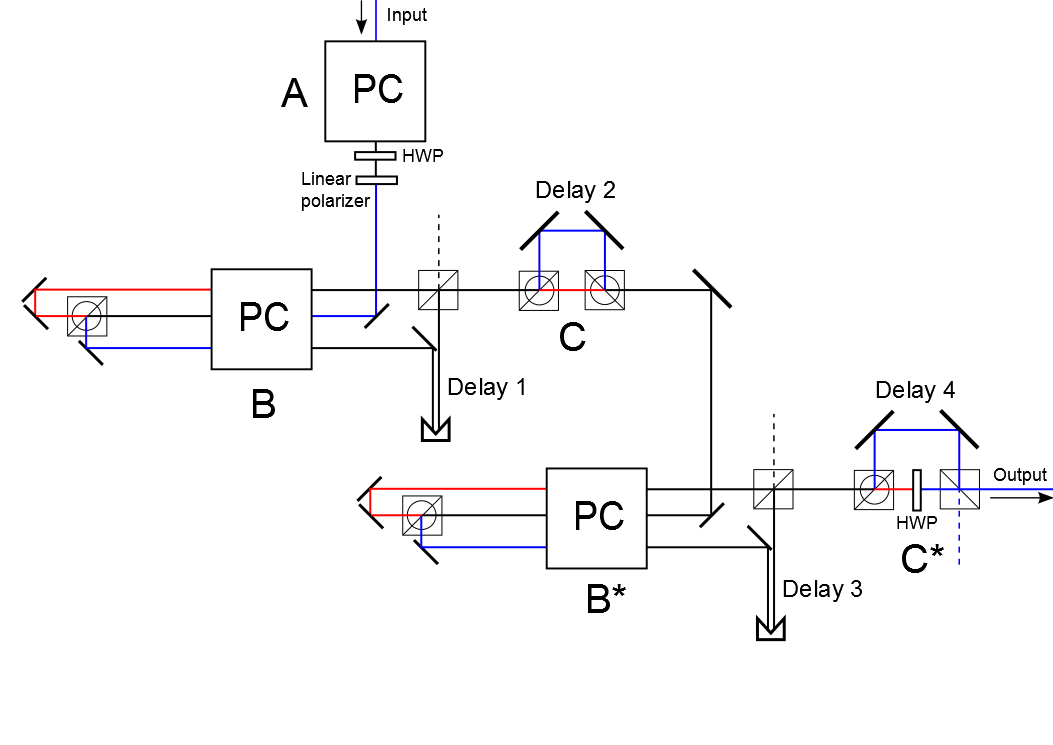
\includegraphics[width=0.8\textwidth]{digitizing.png}
\caption{A schematic of a simplified version of the current design. The network is broken into lettered stages, where the input into the system happens immediately above stage A and the output of the system is returned after stage C*. Stages B and C are repeated twice, where the second occurrences are indicated by B* and C*. Pockels Cell is abbreviated as PC, and half-wave plate is abbreviated as HWP. The squares with a diagonal line and a circle denote a polarizing beam splitter, and the squares without the circle denote are beam splitters. The wedges creating delays 1 and 3 are retroreflectors.  }
\label{fig:digitizing}
\end{figure}

In Figure \ref{fig:digitizing}, there are four different stages denoted with letters A-C. Stages B and C are duplicated (denoted by B* and C*), and the benefit of duplicating these stages is explained later in this section. The delays labeled Delay 1, Delay 2, etc... are the four tunable delays in this design. Adjusting these delays for different sequences increases the precision of the digitizing design. The selection of these times is discussed in Section \ref{sec:optimizing}. Overall, to understand how the network modifies the pulses within each stage, timing diagrams were generated using the simulation tools (to be discussed in more detail in Section \ref{simulation}). In each timing diagram, the ideal pulses are drawn in green dashed lines for reference. 

\subsubsection*{Stage A}

In stage A, the exact number of desired pulses are selected from the laser's immediate output at the times most easily delayed by the network such that the output pulse matches the ideal sequence. The Pockels Cell is used to flip the polarization of the six desired pulses such that those six pulses are horizontally polarized. The half-wave plate flips the polarization of all the pulses so that the six desired pulses are back to being vertically polarized, and the remaining pulses are all horizontally polarized. Finally, the linear polarizer then blocks out the unwanted, horizontally polarized pulses.

\begin{figure}[H]
\centering
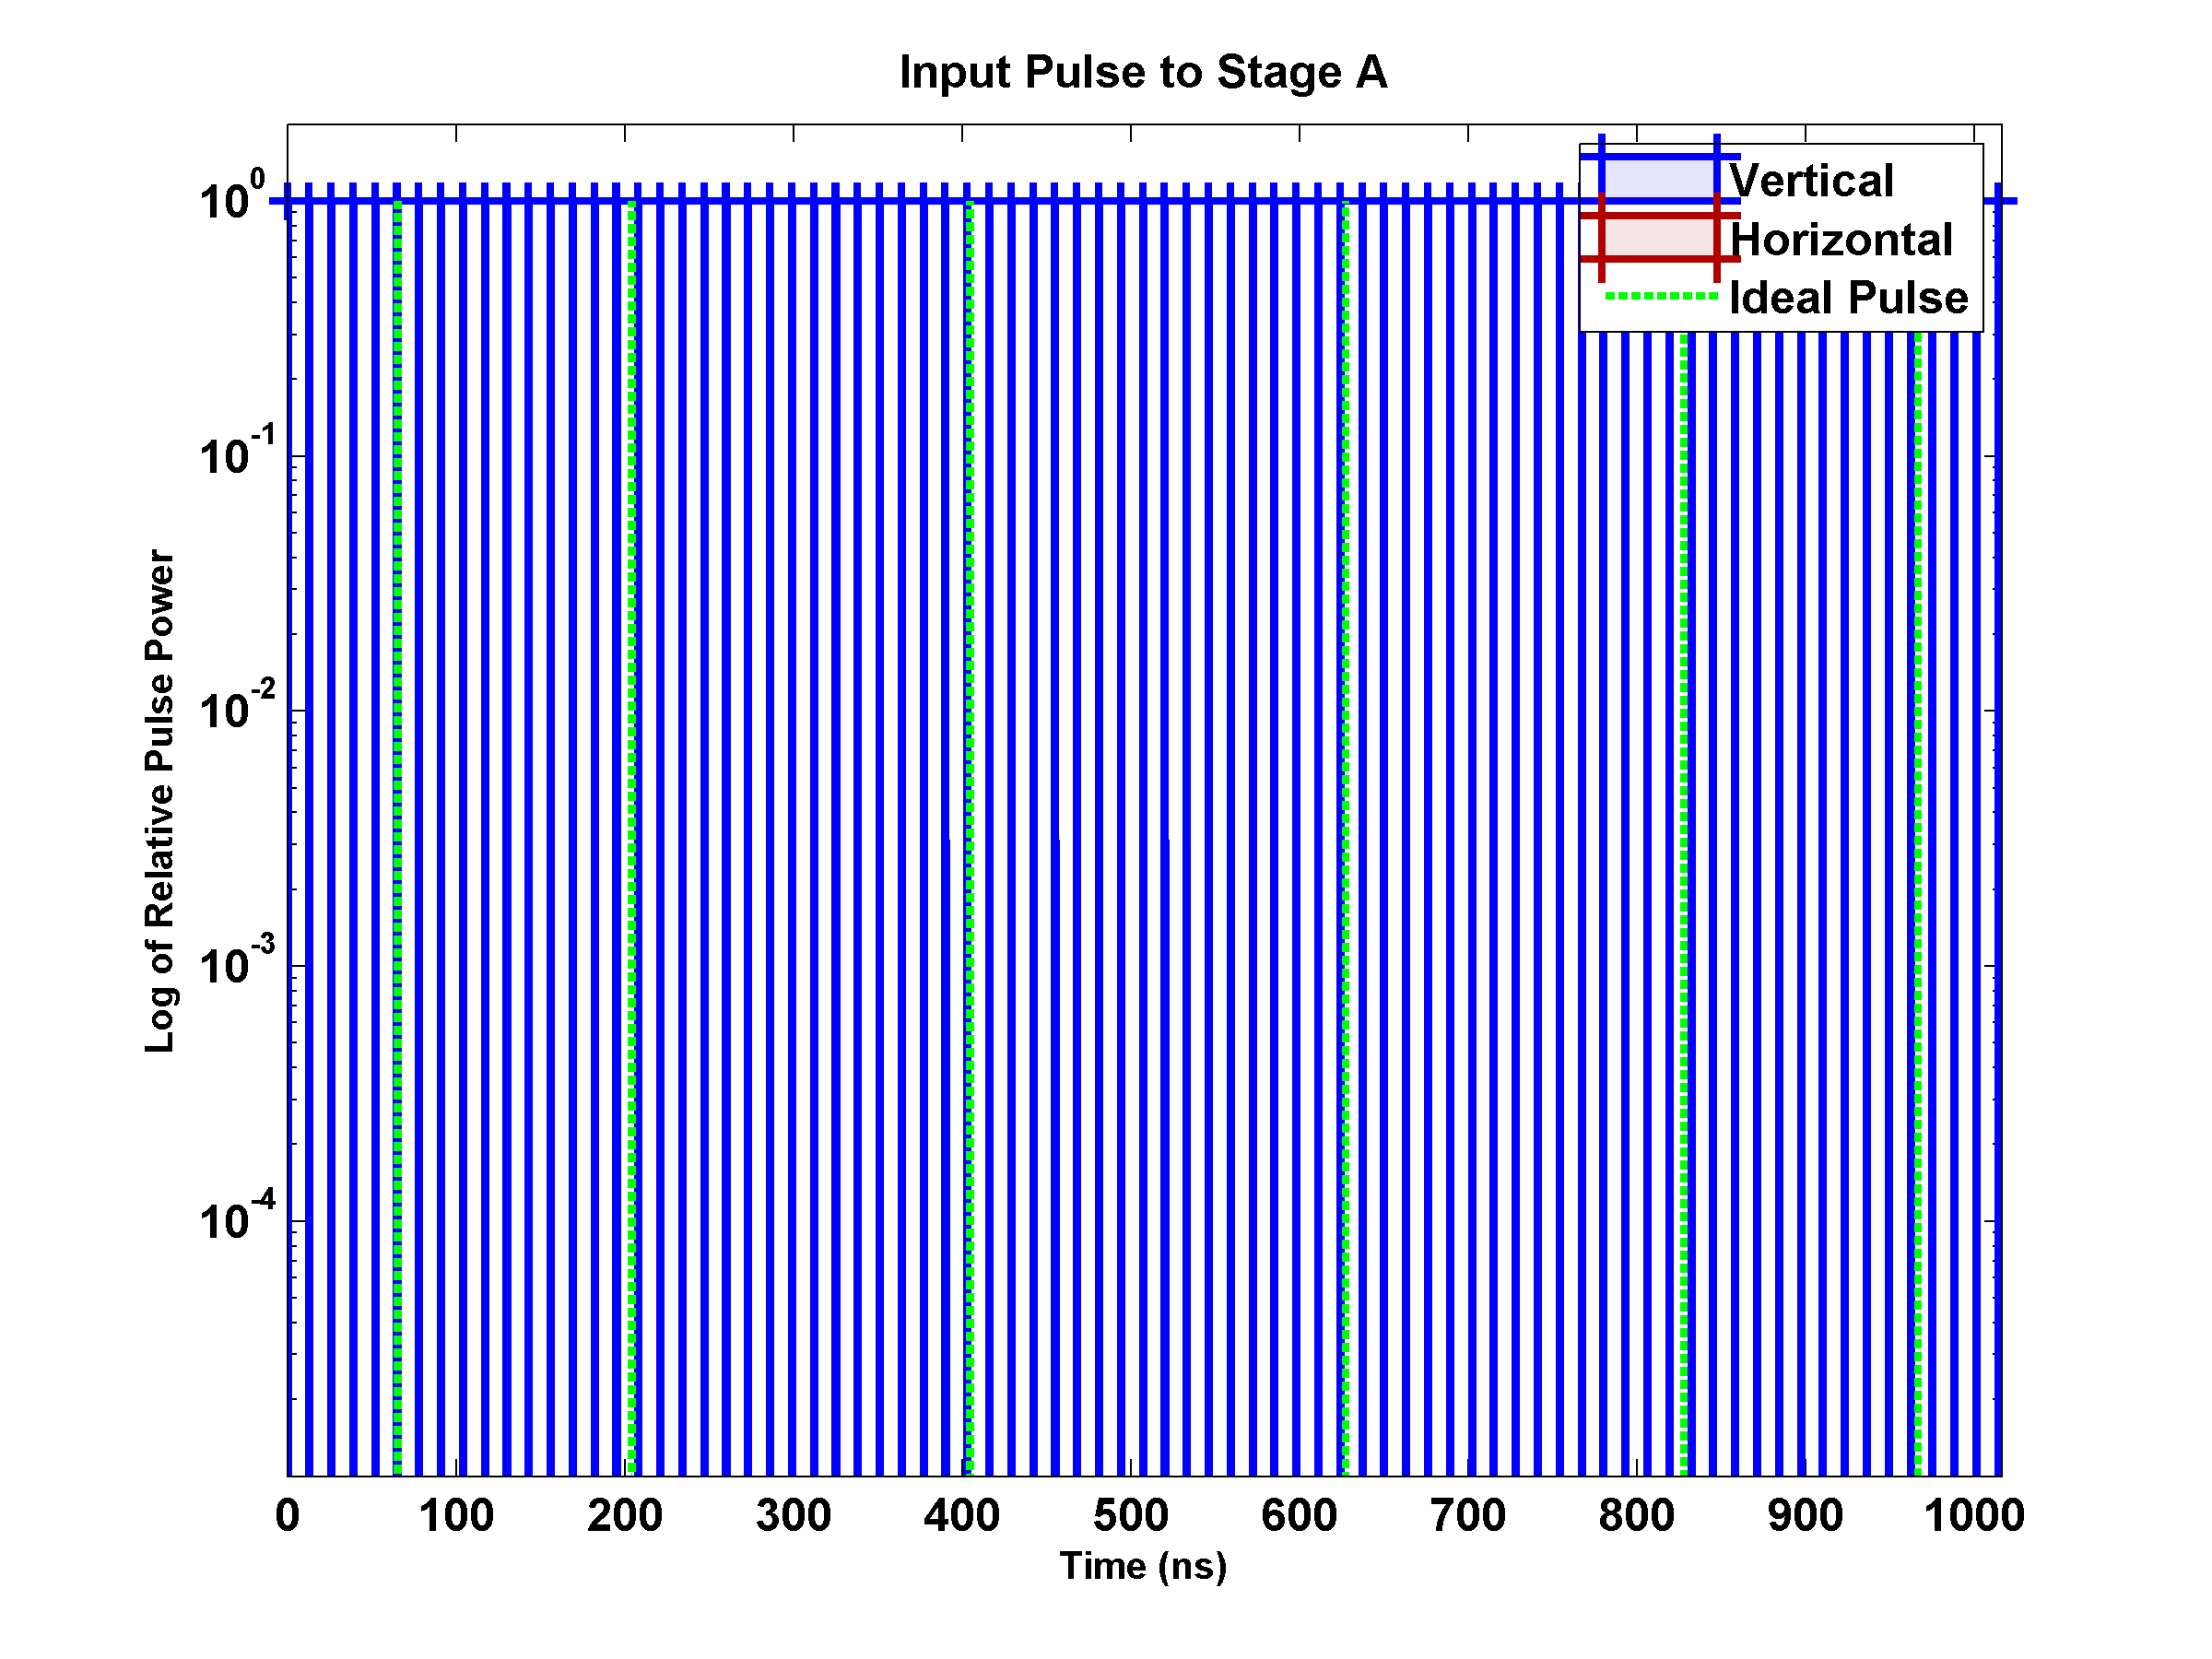
\includegraphics[width=0.8\textwidth]{input_pulse.png} \caption{The blue pulses in this timing diagram represent the pulses being output from the laser with a 13 ns repetition rate. The green, dashed pulses indicate the location of the ideal pulses. The y-axis is an arbitrary measure of the pulses power. This axis is more relevant in later graphs to show relative power loss. The legend denotes that blue pulses have vertical polarization and red pulses (not shown in this image) are horizontally polarized.}
\label{fig:timing_input_train}
\end{figure}

\begin{figure}[H]
\centering
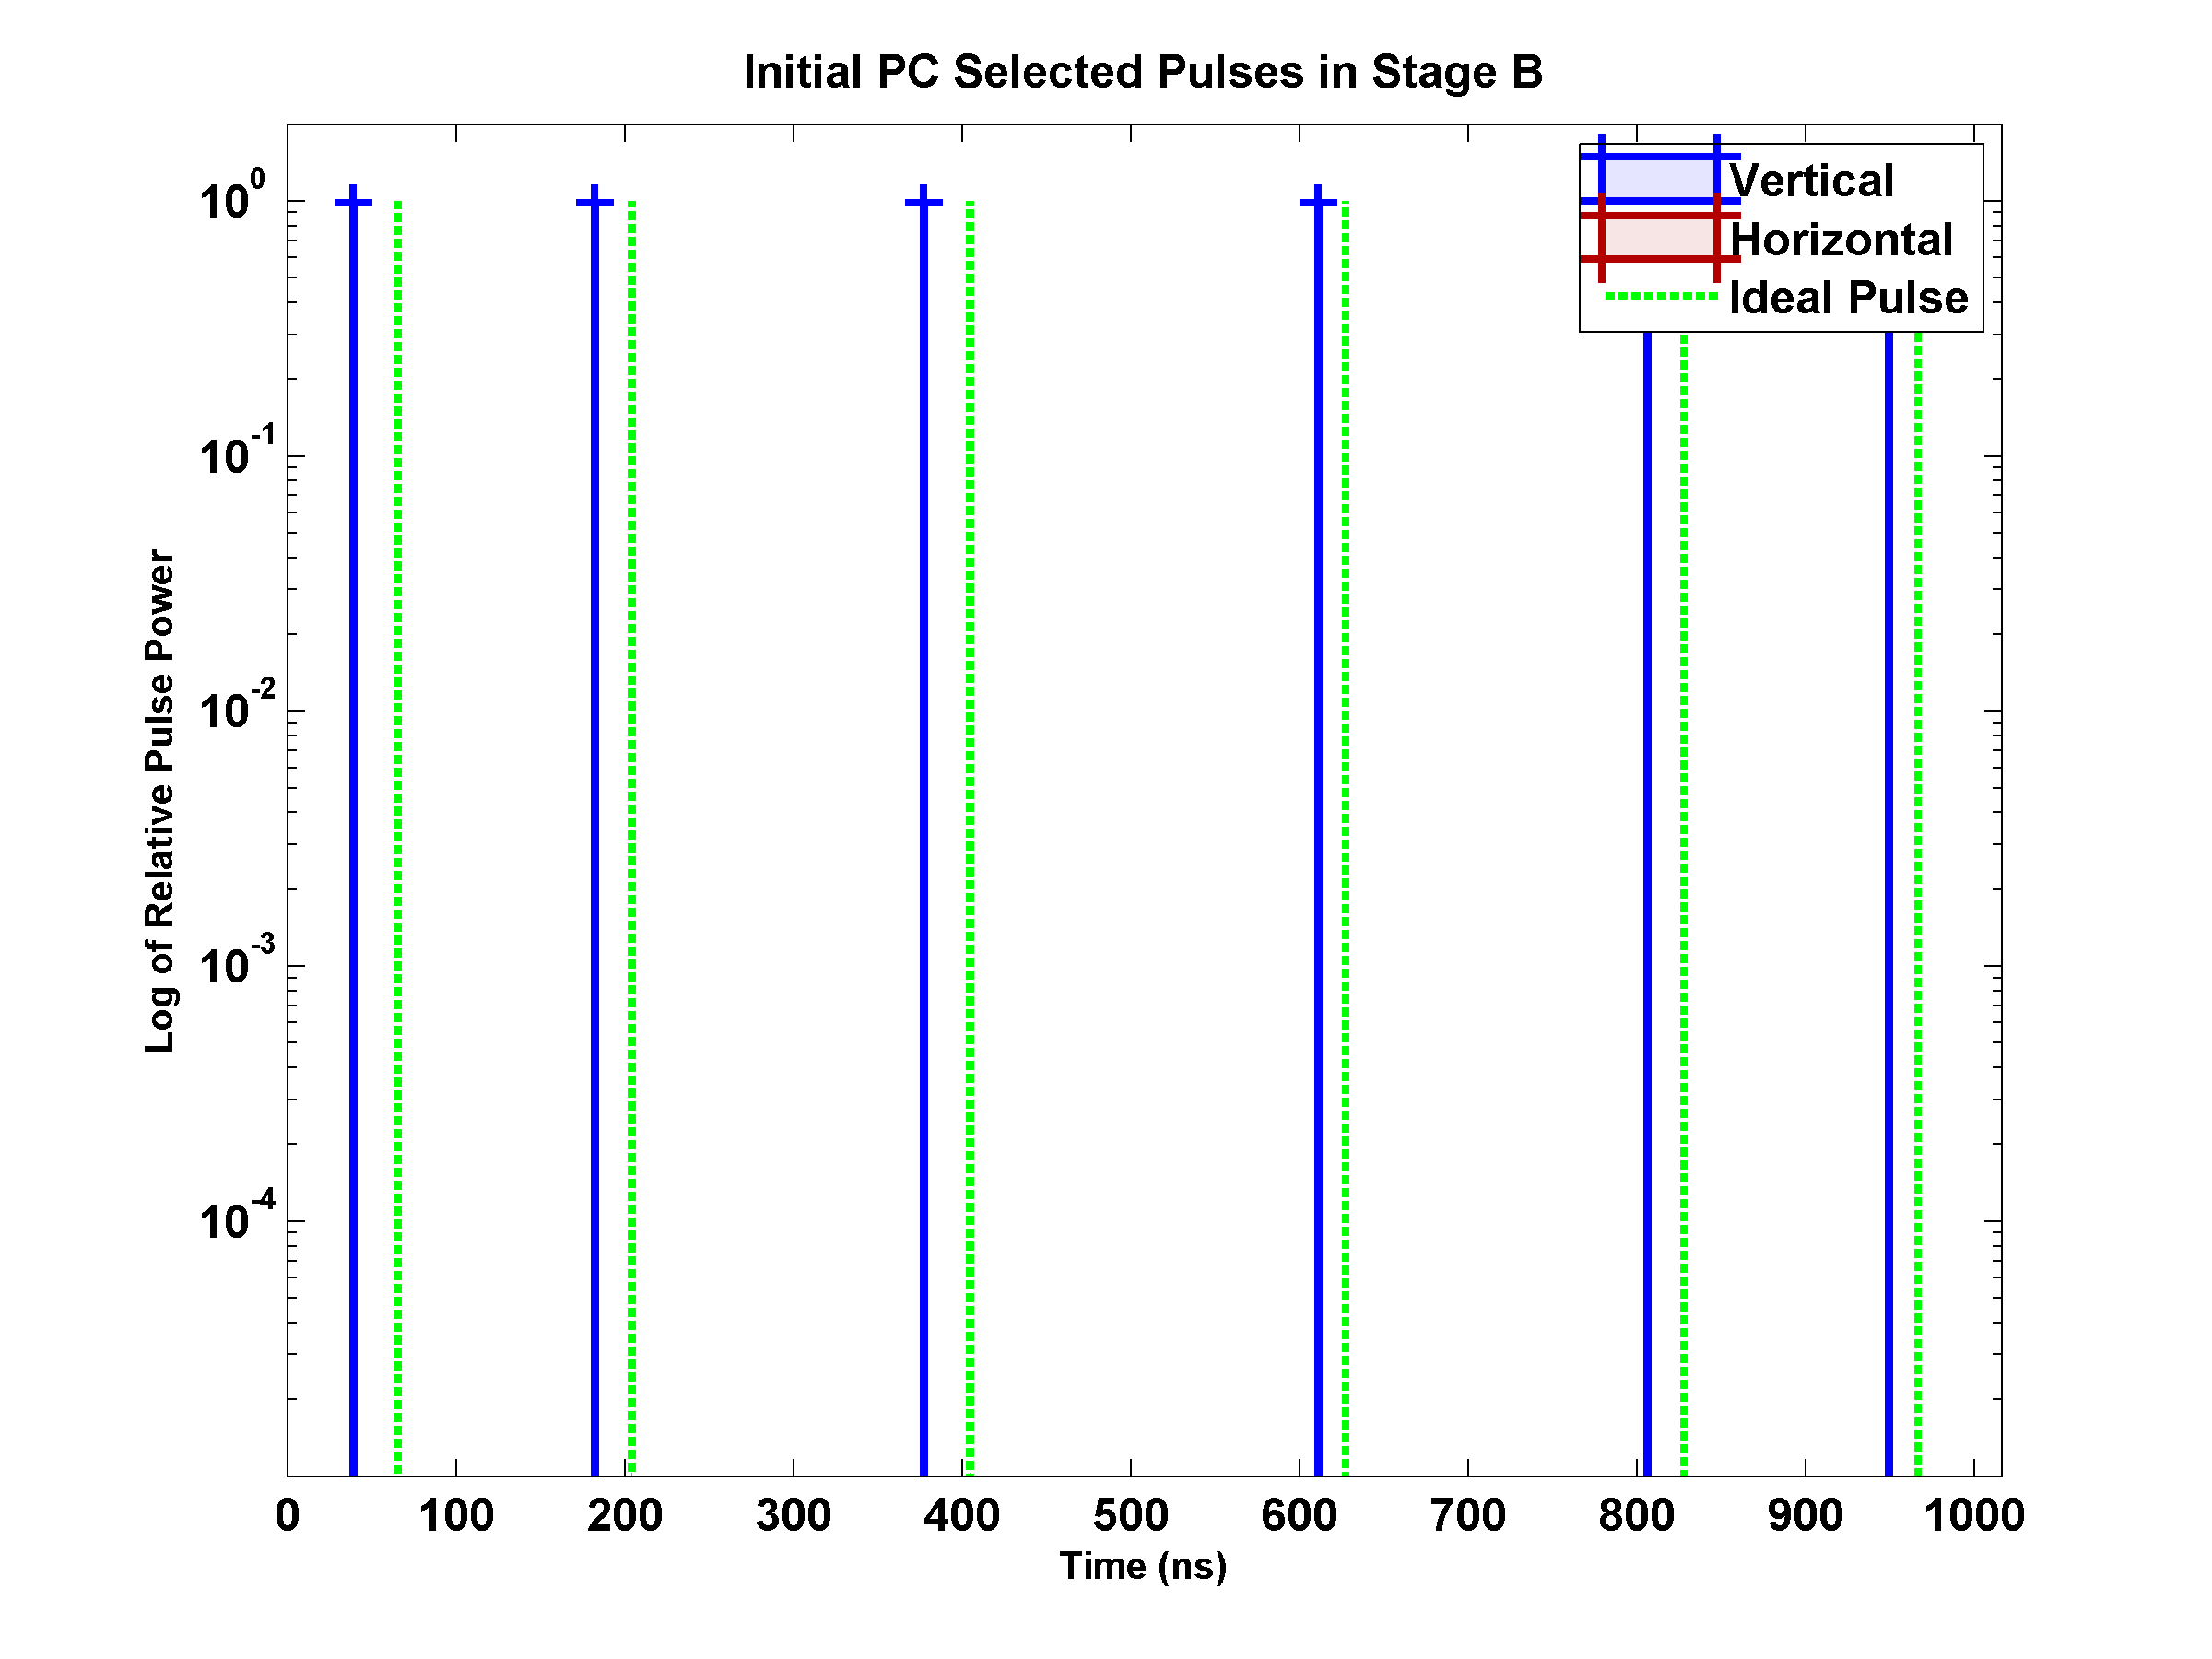
\includegraphics[scale=0.5]{initialEOMOut.png} \caption{This timing diagram represents the output after stage A within Figure \ref{fig:digitizing}. The green pulses indicate the ideal pulses. At this stage the Pockels Cell has selected, from the train of pulses shown previously in Figure \ref{fig:timing_input_train}, the six pulses which can most easily be delayed to match the ideal times. 
}
\label{fig:timing_A}
\end{figure}


\begin{figure}[H]
\centering
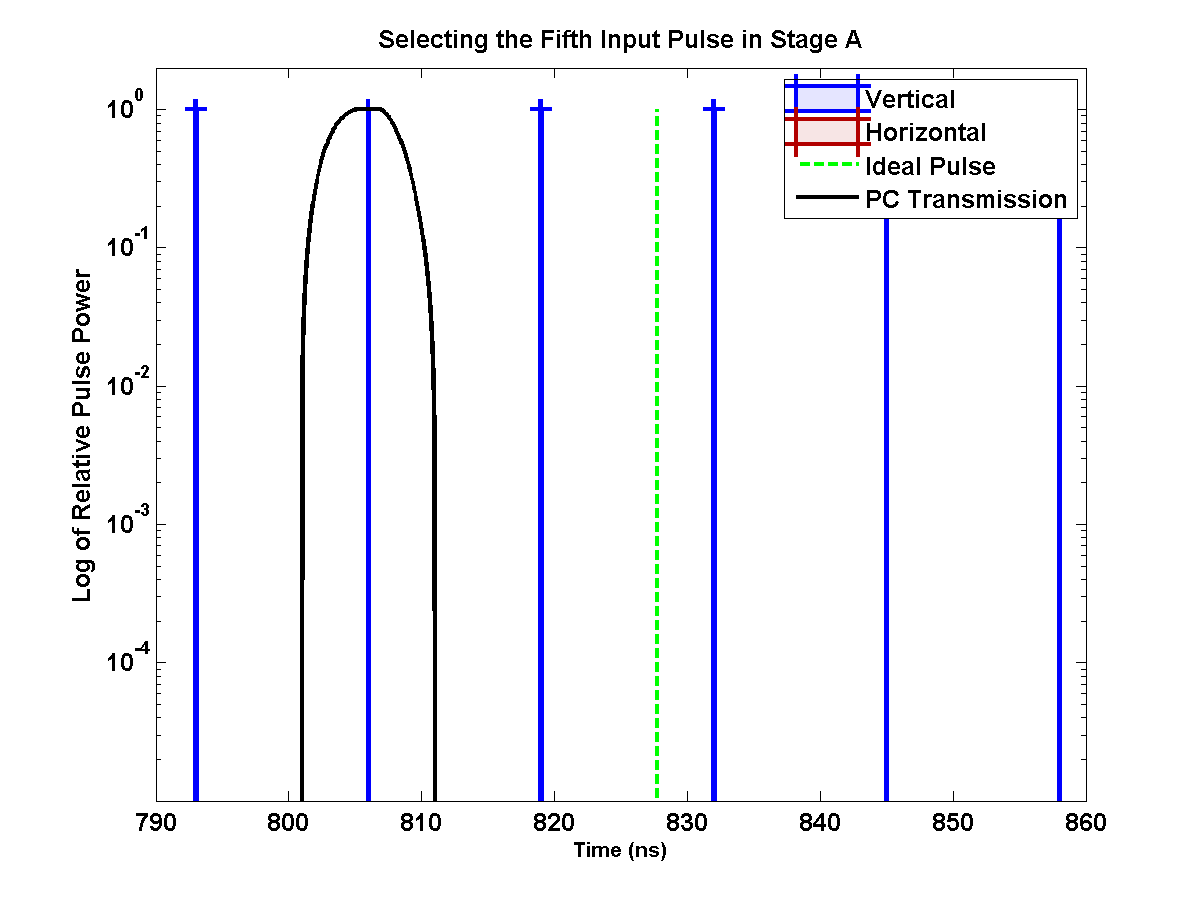
\includegraphics[scale=0.5]{pulse5Selection.png} \caption{This timing diagram is a close up of the selection of pulse 5. The black curve represents when the Pockels Cell is on, which is when the polarization of the pulse is flipped. After the Pockels Cell flips this pulse, the half-wave plate flips the polarization of every pulse, restoring this pulse to a vertical polarization and leaving everything else horizontal. The linear polarizer is then used to block the horizontal pulses. These components in conjunction work to select this desired pulse. }
\label{fig:pulse5_A}
\end{figure}

 As shown in Figure \ref{fig:timing_input_train}, the input into stage A from the rotation laser has evenly spaced pulses with a repetition rate of 13 ns. In this figure, and all the subsequent timing diagrams, blue pulses denote vertical polarization and red pulses denote horizontal polarization. The y-axis is pulse power, normalized to the input laser pulse power. In Figure \ref{fig:timing_A}, the output from stage A shows the six pulses which can most easily be delayed to form the ideal sequence. Figure \ref{fig:pulse5_A} zooms in to visualize the selection of an individual pulse, pulse 5. The black transmission curve represents the rise and fall time of the Pockels Cell. This transmission curve is directly related to the amount by which the Pockels Cell flips the polarization of light passing through. At zero, the Pockels Cell doesn't change the input polarization, and at one, the Pockels Cell flips the polarization completely, barring realistic imperfections in the component. The details of the specific Pockels Cell and the imperfection used in simulation can be found in Section \ref{simulation}. Each Pockels Cell curve is centered about the pulse which is selected to be delayed to the ideal sequence. 

\subsubsection*{Stage B}
In this stage, the network manipulates the pulses so that they can undergo the desired delays and be moved as close to the ideal timings as possible. This is accomplished by passing each pulse through a Pockels Cell twice, as seen in Figure \ref{fig:stageB}. The first pass determines which branch the pulse follows, and the second pass sets the pulse's polarization for the rest of the sequence. Since certain delays only affect certain branches or certain polarizations, using the Pockels Cell in this manner allows different pulses to accumulate different delays. 


\begin{figure}[H]
\centering
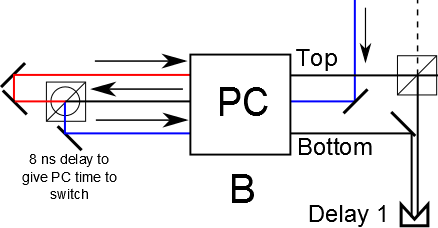
\includegraphics[scale=0.6]{stageB.png} 
\caption{This schematic is stage B from Figure \ref{fig:digitizing}. This section uses the technique of double-passing the pulses through the Pockels Cell to select different pulses for different delay combinations.}
\label{fig:stageB}
\end{figure}

In Figure \ref{fig:stageB}, the six pulses enter Stage B at the top arrow. The line is blue to denote purely vertically polarized pulses. After exiting the Pockels Cell the first time, some pulses are vertically polarized and others are horizontally polarized. The polarizing beam splitter sends all horizontal pulses to the top branch and the vertical pulses to the bottom. During the path out of the Pockels Cell, through the polarizing beam splitter, and back into the Pockels Cell a second time, the pulses all experience an 8 ns delay. This delay is not one of the tunable delays used to modify individual pulses since it is applied to all pulses. Its purpose is to give the Pockels Cell enough time to rise and fall such that it could flip a pulse arriving in one direction and have enough time to turn off and not flip the pulse as it returns on its second pass, or vice versa. As both branches re-enter the Pockels Cell for the second time, the polarization of each pulse is determined. After exiting the Pockels Cell, the bottom branch receives an additional delay, denoted as Delay 1 in Figure \ref{fig:stageB}. For this particular sequence, Delay 1 is 6.5 ns. Finally, the bottom branch is recombined with the top branch. By the time the two branches are combined, there are four possible states for the pulses: 1) vertical, 2) vertical and delayed, 3) horizontal, 4) horizontal and delayed. 


\begin{figure}[H]
\centering
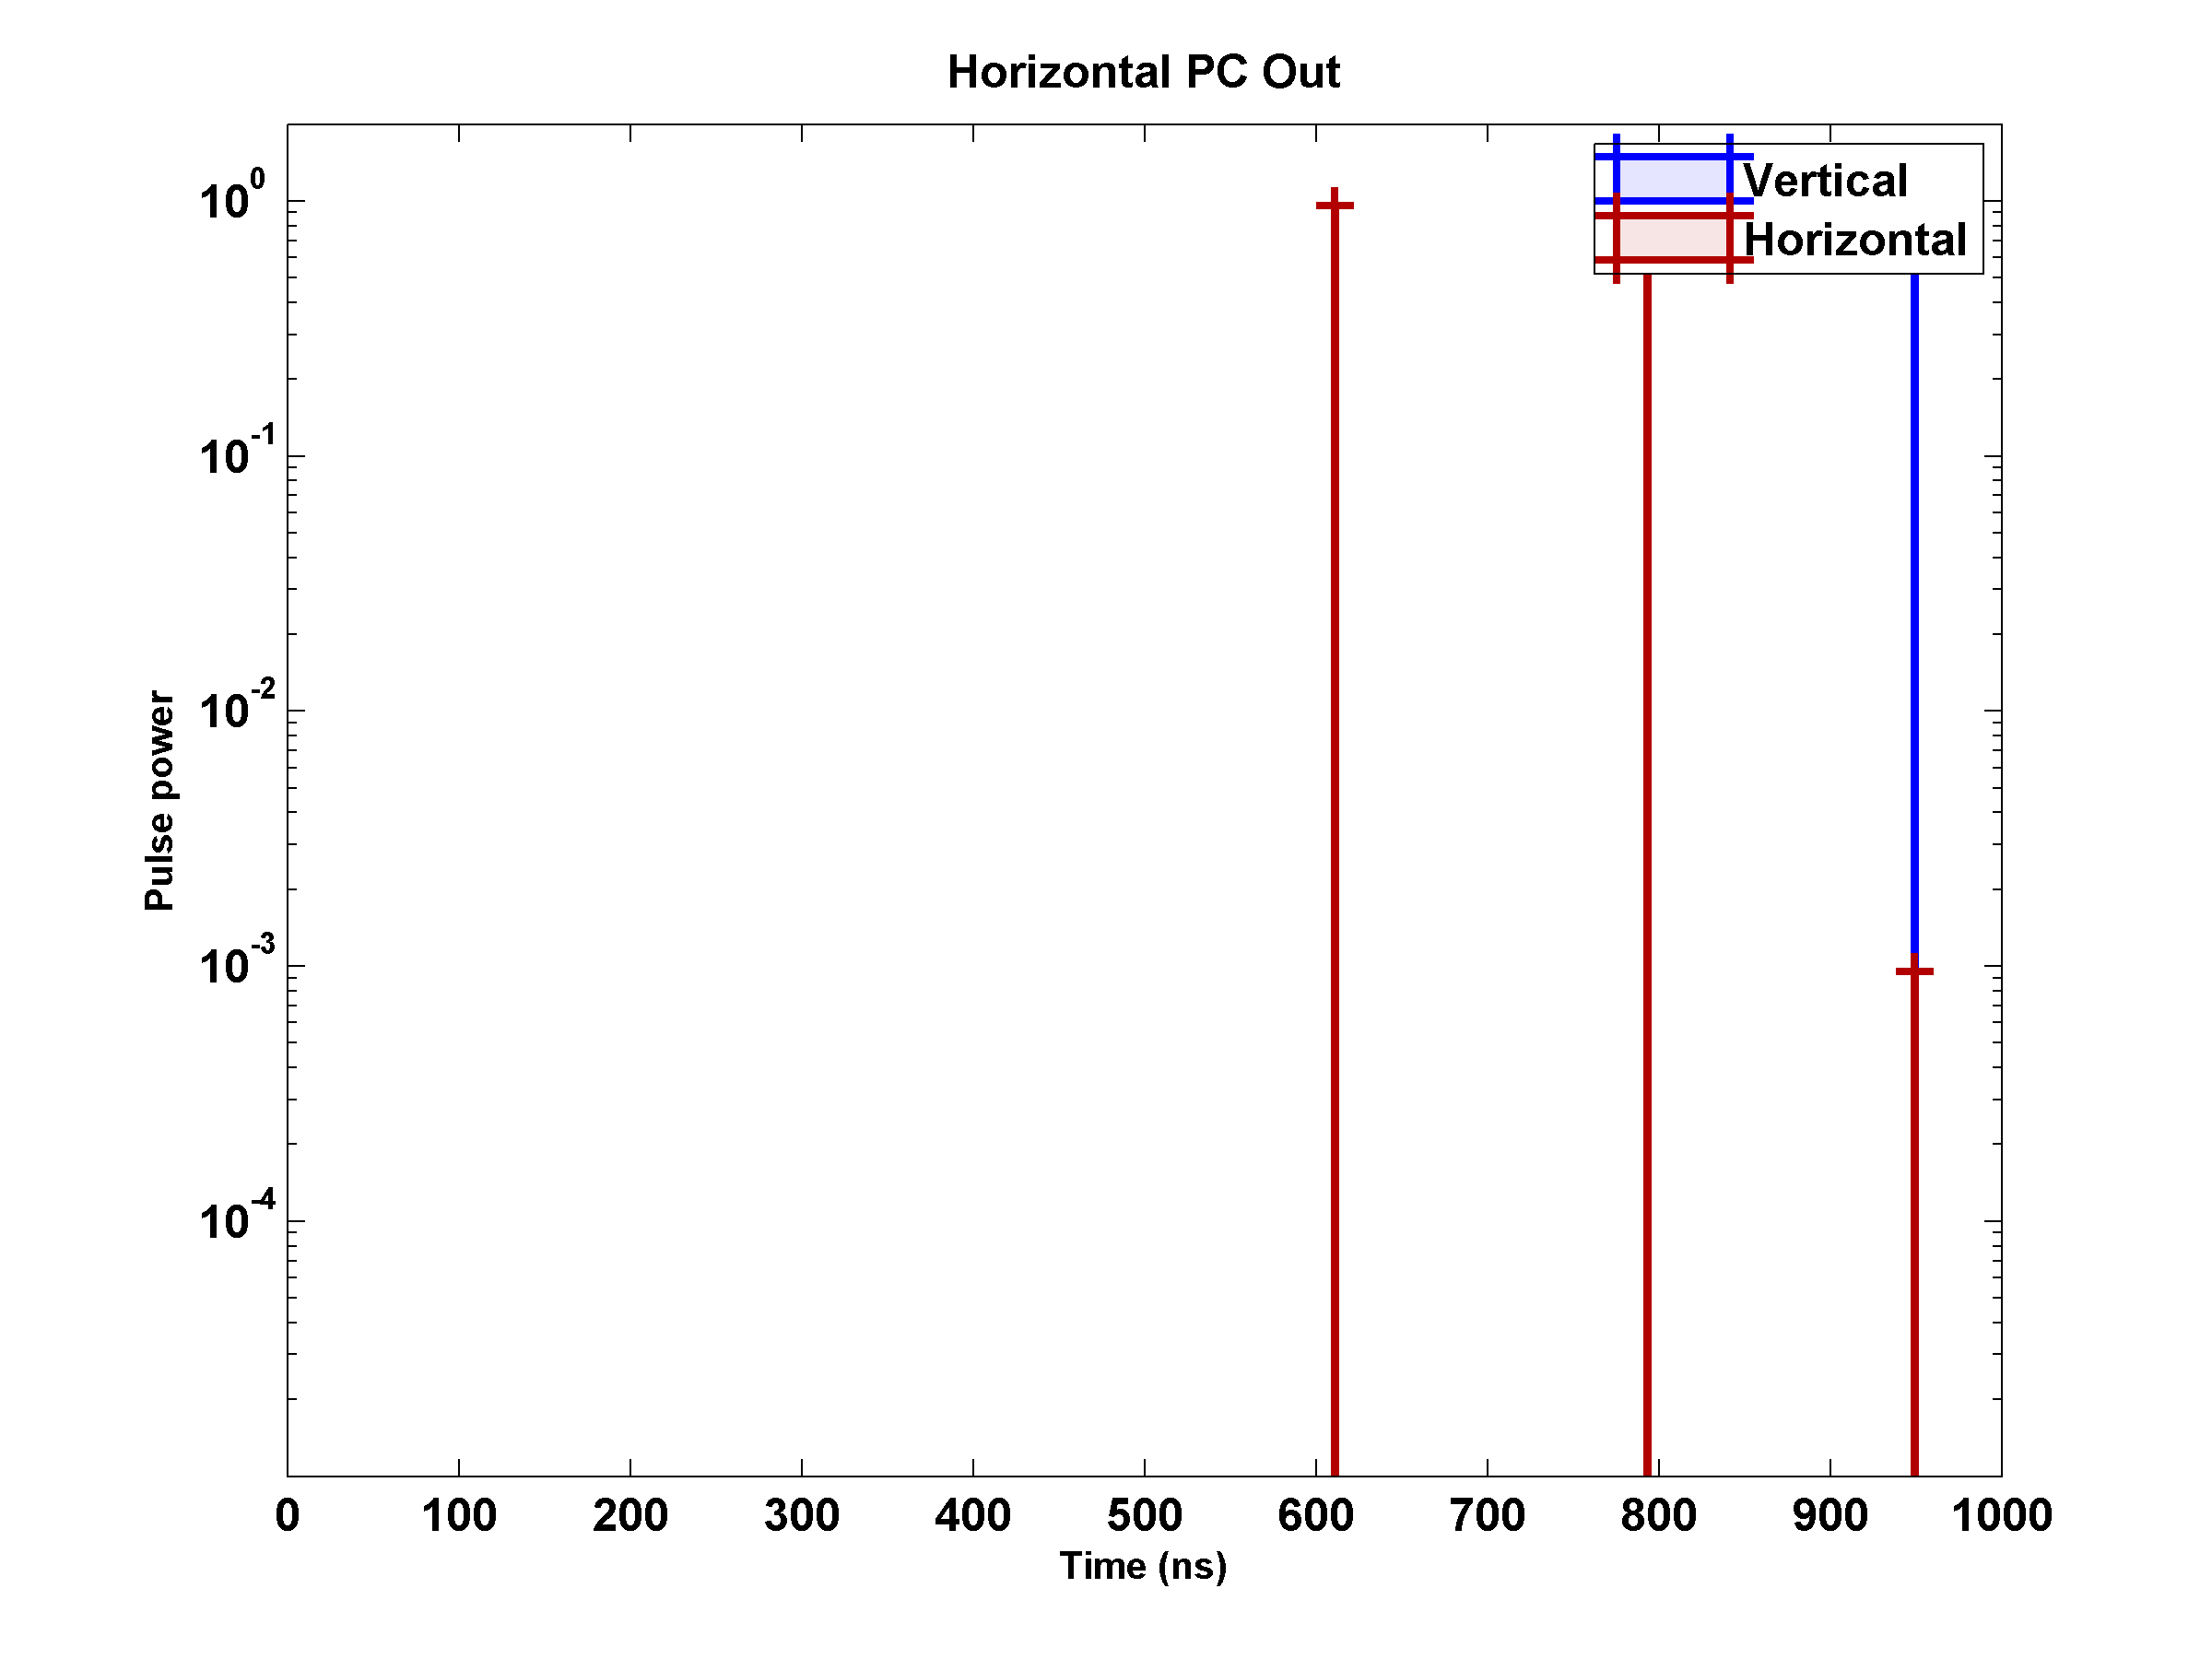
\includegraphics[scale=0.6]{horizPCOut.png} \caption{This timing diagram shows the pulses coming out of the ``Top" branch of Figure \ref{fig:stageB}. The last pulse was flipped on its second pass to return it to a vertical polarization. These pulses do not receive Delay 1, so their states are horizontal, horizontal, and vertical. The significantly attenuated horizontal component of the last pulse is from simulating inefficiencies in the Pockels Cell and will be discussed further in Section \ref{simulation}. Note that the y-axis is on a log scale.}
\label{fig:timing_B1}
\end{figure}

\begin{figure}[H]
\centering
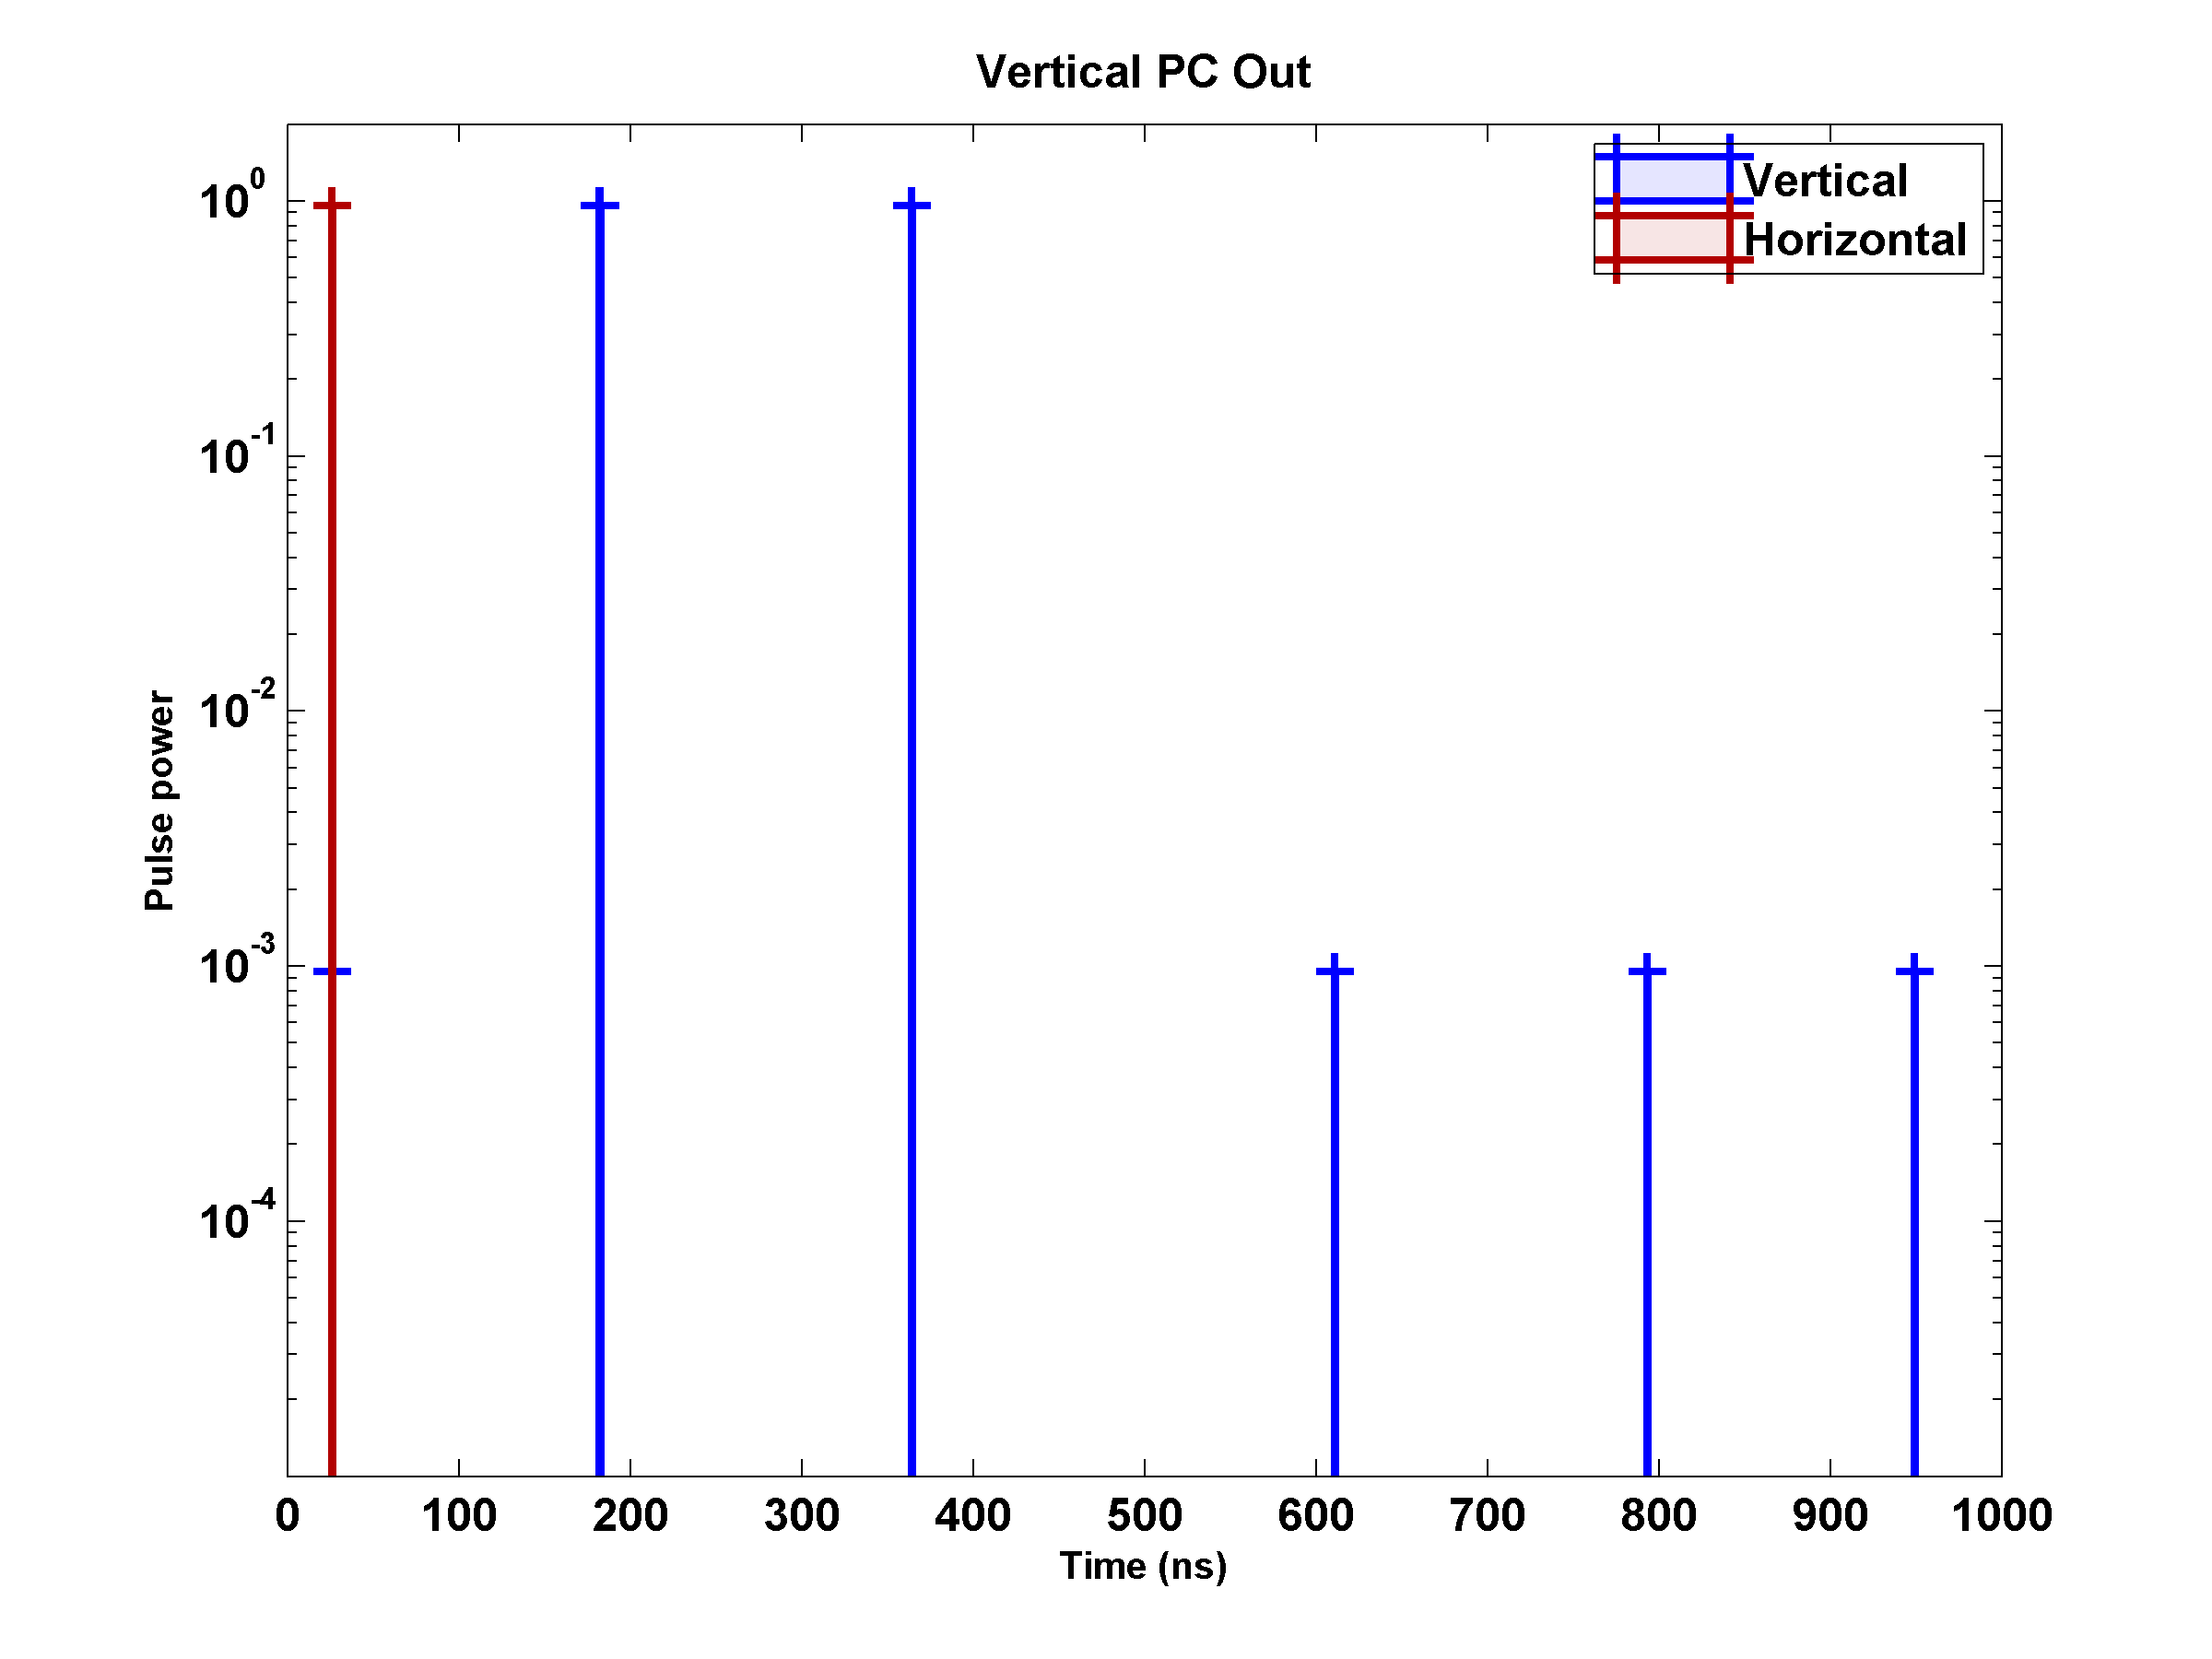
\includegraphics[scale=0.6]{vertPCOut.png} \caption{This timing diagram shows the pulses coming out of the ``Bottom" branch of Figure \ref{fig:stageB}. The first pulse was flipped on its second pass, leaving it with horizontal polarization. These pulses do receive Delay 1, so their states are horizontal-delayed, vertical-delayed, and vertical-delayed. The significantly attenuated vertical pulses after 500 ns are from modeling inefficiencies in the Pockels Cell.}
\label{fig:timing_B2}
\end{figure}

\begin{figure}[H]
\centering

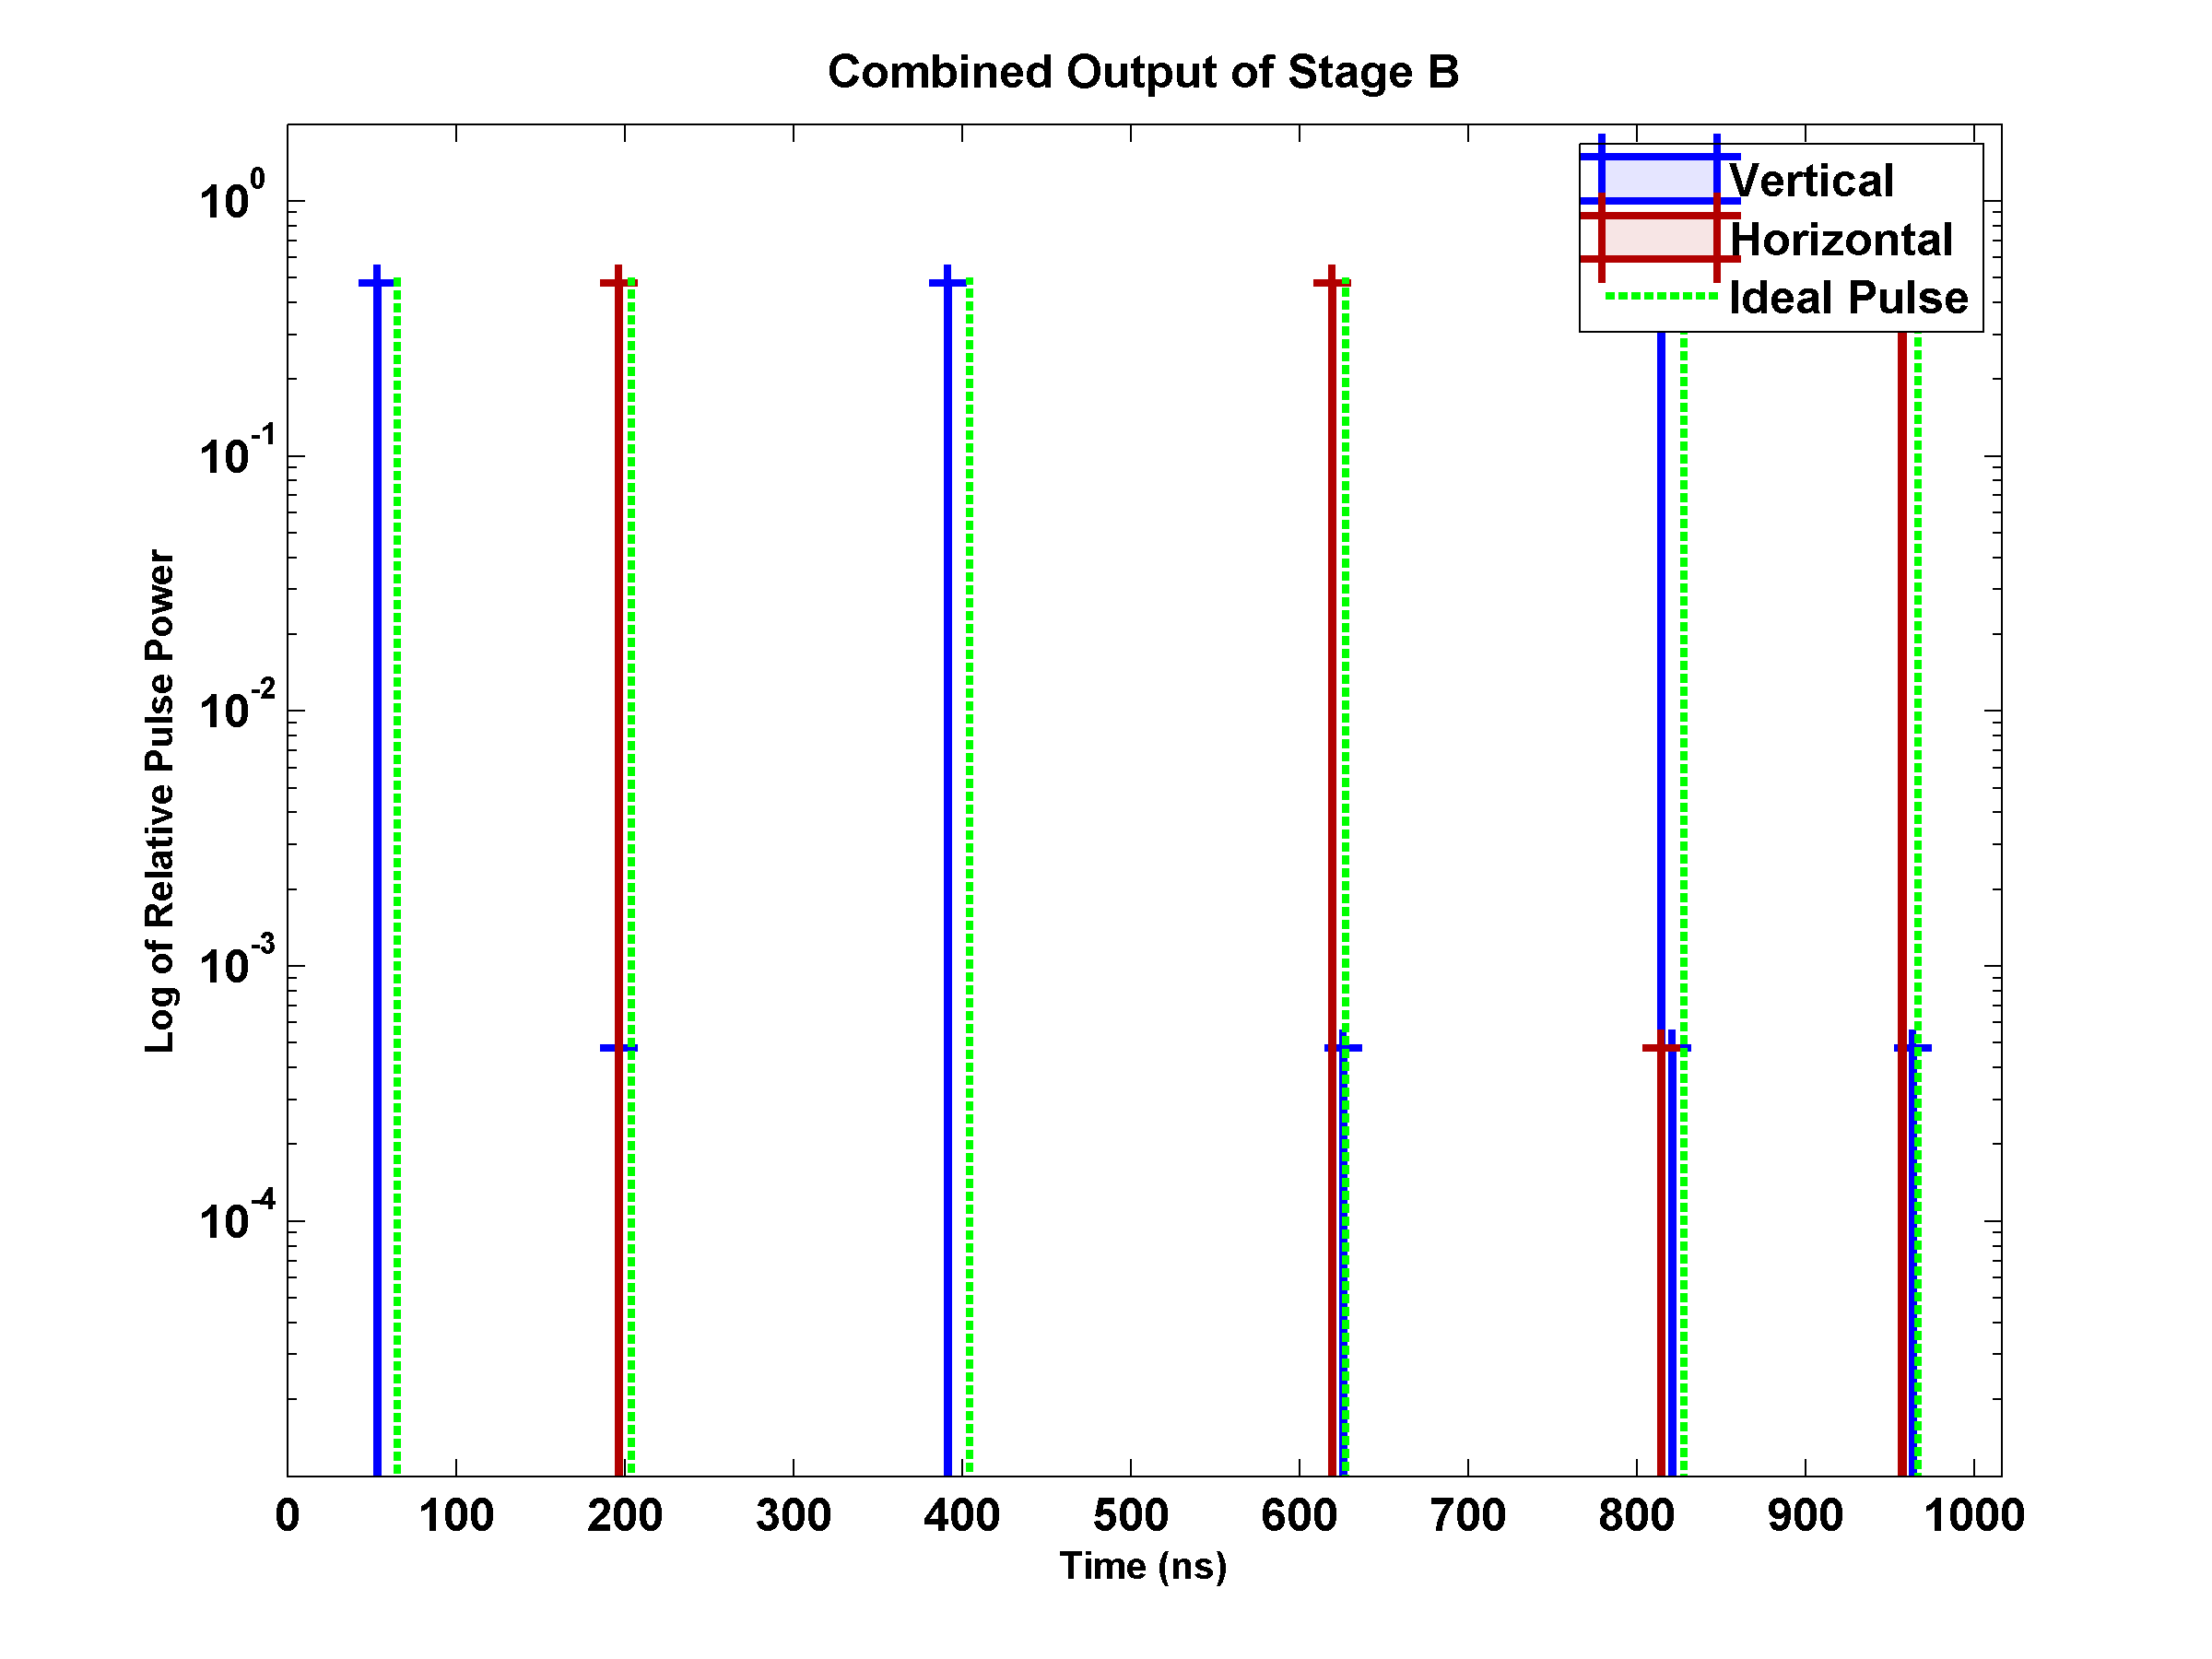
\includegraphics[scale=0.6]{RotatedPulses.png} \caption{This timing diagram shows the pulses after the ``Top" and ``Bottom" branches from Figure \ref{fig:stageB} have been recombined. The green pulses are shown to compare the modified pulses to the ideal pulses. The additional small pulses are from modeling Pockels Cell inefficiencies.}
\label{fig:timing_B3}
\end{figure}

Figure \ref{fig:timing_B1} and Figure \ref{fig:timing_B2} represent the ``Top'' and ``Bottom'' branches of the Pockels Cell output, respectively. Figure \ref{fig:timing_B3} shows the separate branches from the Pockels Cell recombined into one path. This double-passed Pockels Cell sets the states of each pulses as follows: pulse 1 (horizontal-delay), pulse 2 (vertical-delay), pulse 3 (vertical-delay), pulse 4 (horizontal), pulse 5 (horizontal), and pulse 6 (vertical). 

\subsubsection*{Stage C}

Figure \ref{fig:stageC} represents stage C from Figure \ref{fig:digitizing}, and shows two polarizing beam splitters being used together to create a delay, labeled as Delay 2. In this particular sequence, Delay 2 was chosen to be 3.25 ns. The first polarizing beam splitter sends the vertically polarized pulses down this delay path of 3.25 ns. After the vertically polarized pulses are delayed, they rejoin the horizontal pulses, as seen in Figure \ref{fig:timing_C}. Figure \ref{fig:pulse5_C} focuses on one pulse to more clearly see the effect of this delay.

\begin{figure}[H]
\centering
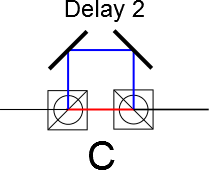
\includegraphics[scale=.7]{stageC.png} 
\caption{This schematic is stage C from Figure \ref{fig:digitizing}. This section uses two polarizing beam splitters to delay the vertically polarized pulses by the value of Delay 2. For this pulse sequence, Delay 2 is 3.25 ns. The output of this stage recombines both the vertical and horizontal pulses.}
\label{fig:stageC}
\end{figure}


\begin{figure}[H]
\centering
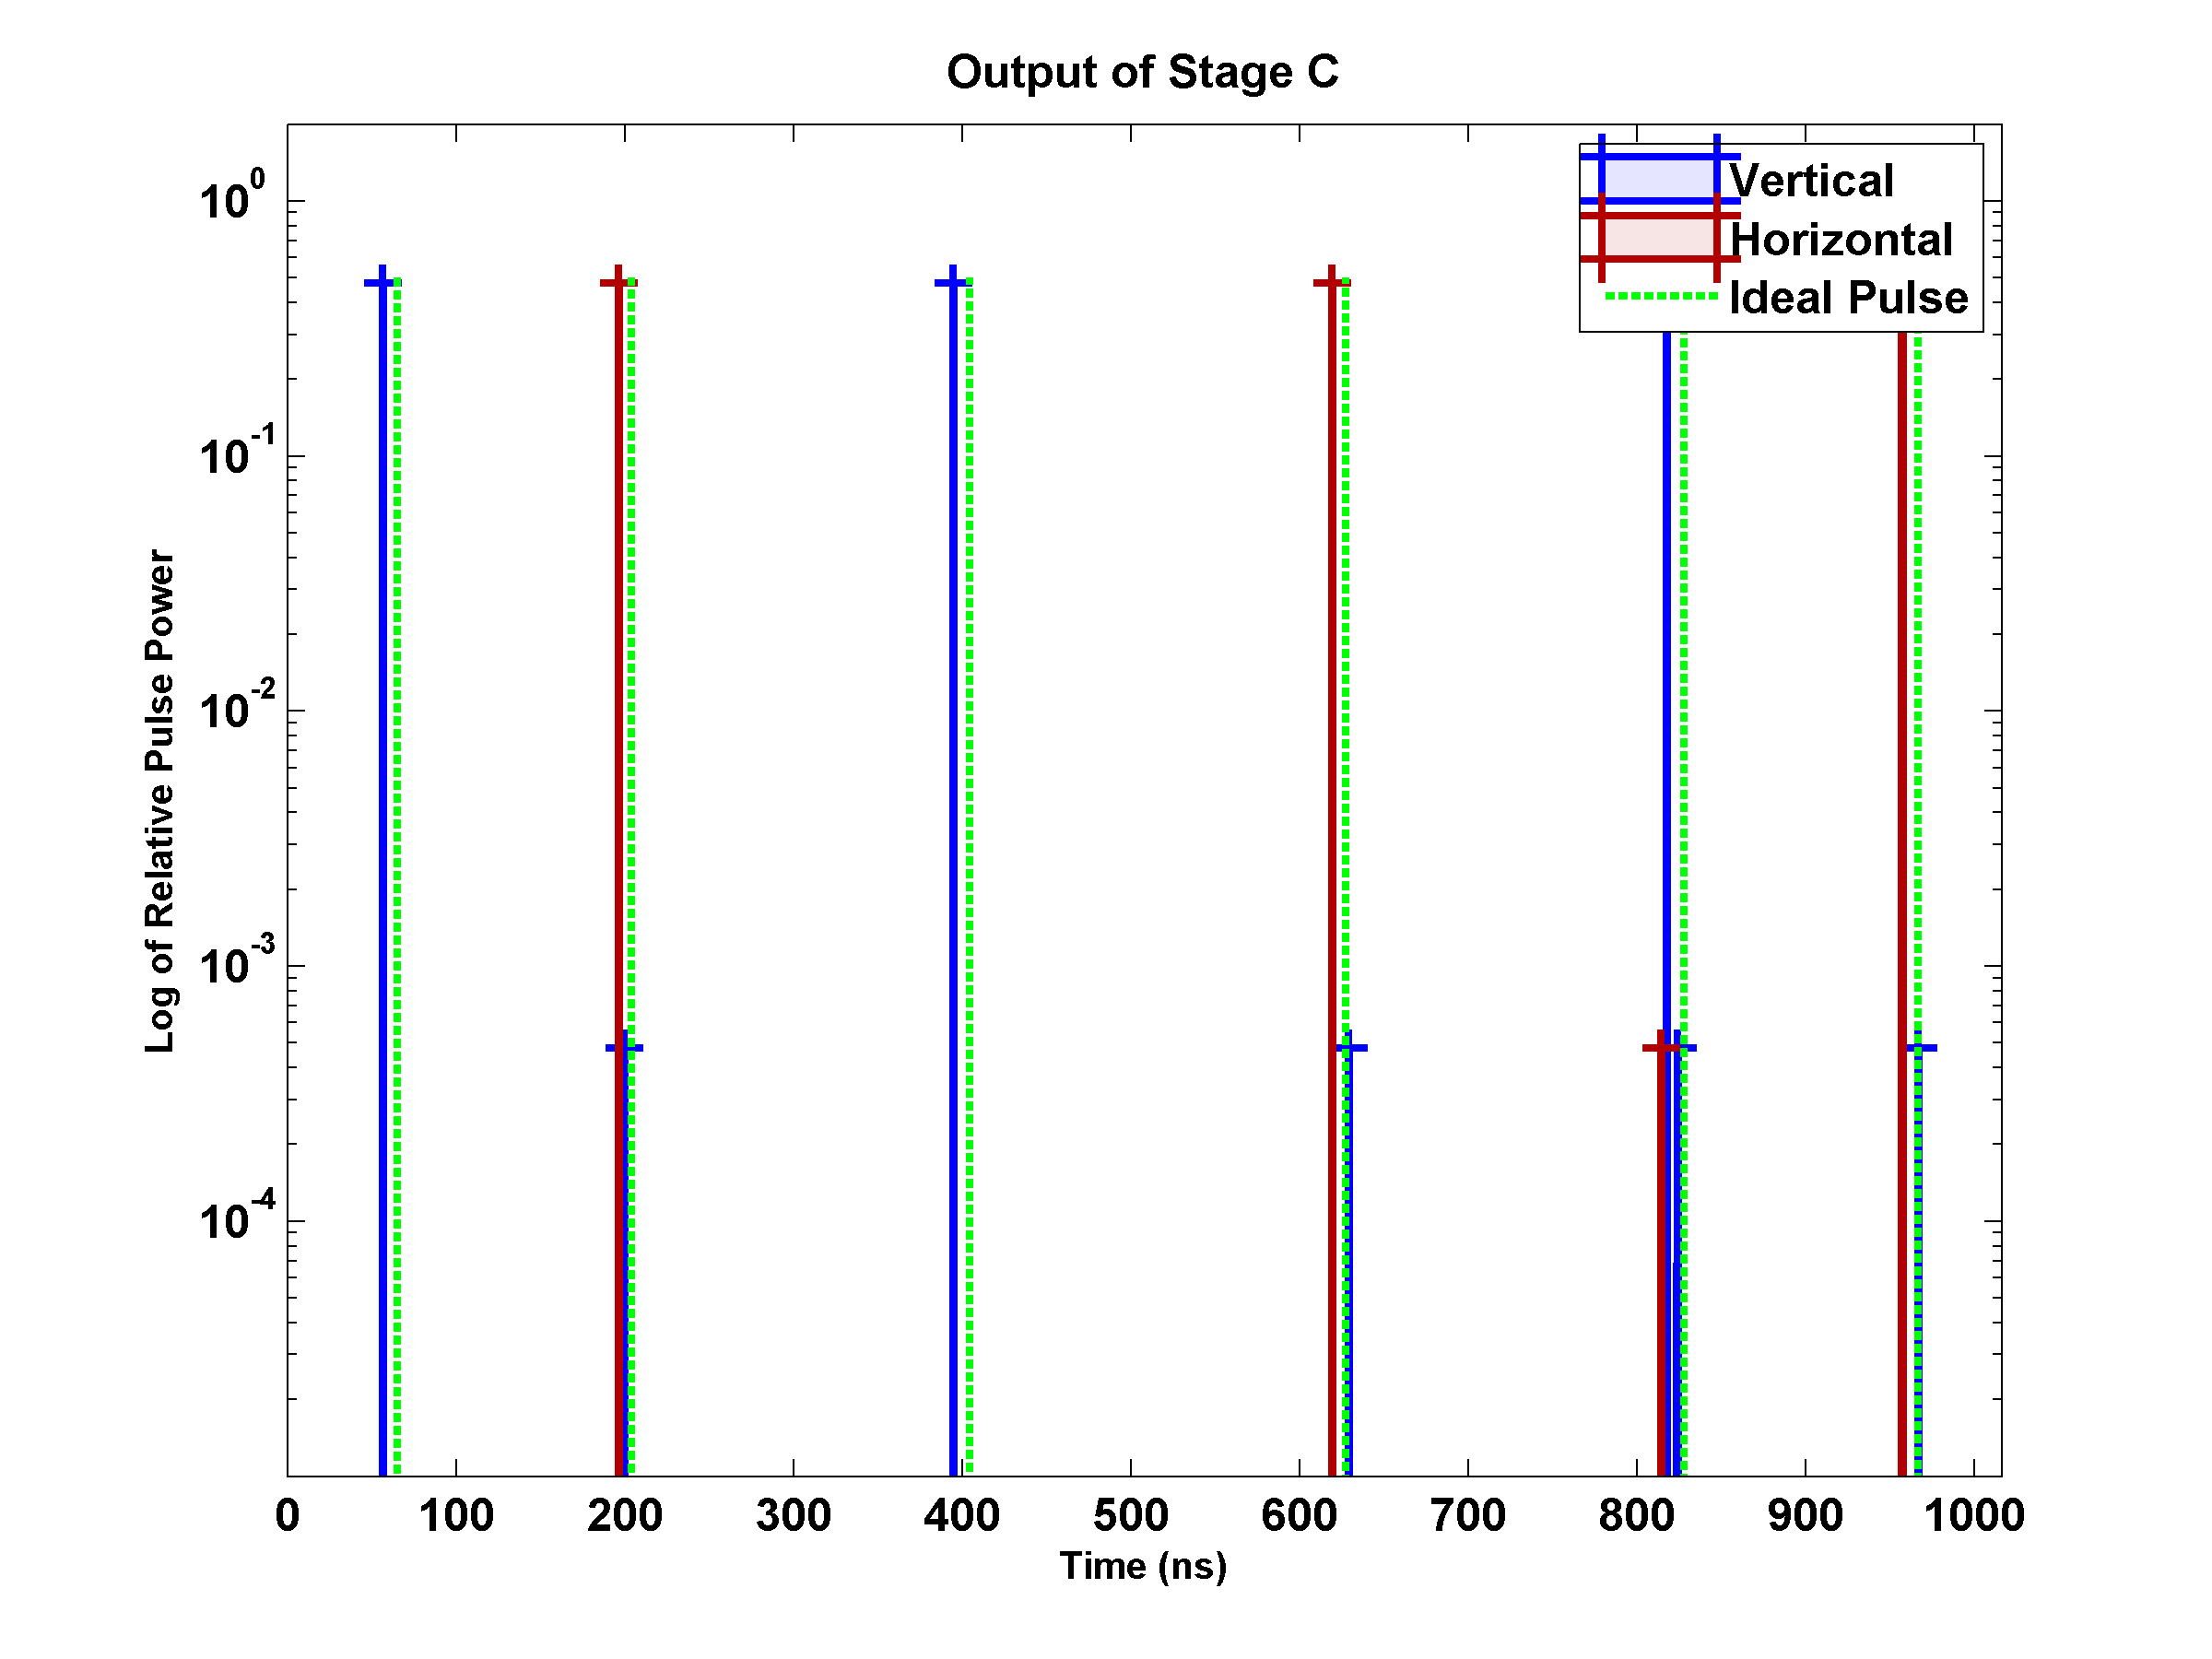
\includegraphics[scale=0.6]{PBSDelayOut.png} \caption{This timing diagram shows the pulses coming out of the polarizing beam splitter delay. The vertically polarized pulses (in blue) have been delayed slightly to approach the ideal times (denoted as green pulses). The additional small pulses are from modeling Pockels Cell inefficiencies.}
\label{fig:timing_C}
\end{figure}


\begin{figure}[H]
\centering
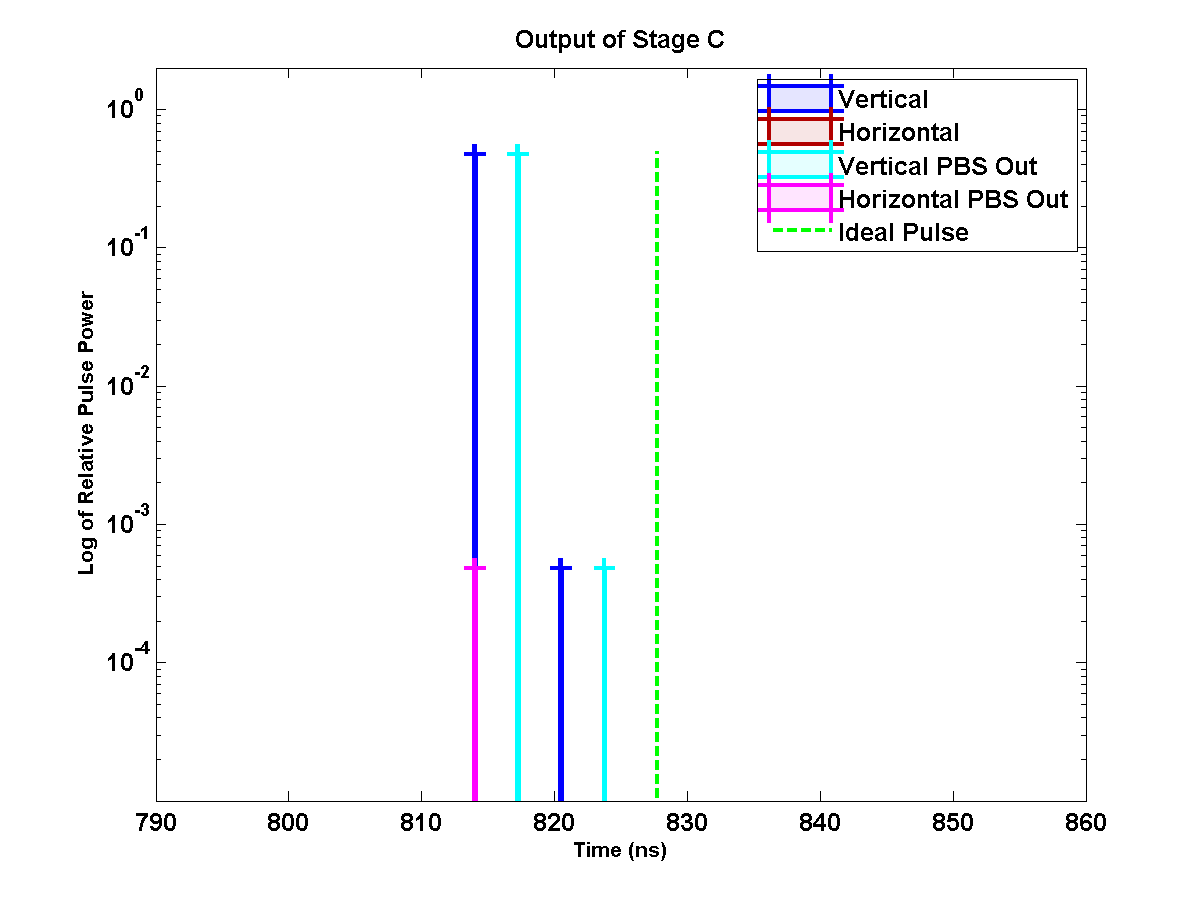
\includegraphics[scale=0.6]{pulse5PBSOut.png} \caption{This timing diagram shows pulse 5 before and after the polarizing beam splitter delay. Pulse 5 is vertically polarized so the input and output are separated by 3.25 ns, or Delay 2. A smaller residual vertically polarized pulse, from modeling Pockels Cell inefficiencies, is also shown to be shifted by the 3.25 ns delay. The residual horizontal pulse (Horizontal PBS Out) also comes from modeling Pockels Cell inefficiencies and does not experience Delay 2.}
\label{fig:pulse5_C}
\end{figure}

\subsubsection*{Stages B* and C*}

From Figure \ref{fig:digitizing}, the next step after stage C is to repeat stages B and C again (shown as stages B* and C*), before reaching the final output. Stages B and C allow the pulses to be in four states, based on their polarization and delay. The output from stage C is directed back into a duplicate of stage B. Stage B* works in the same manner as stage B, except the timings at which this Pockels Cell flips polarizations are different. Stage C is also duplicated, following stage B*. In stage C*, the slight difference is that a half-wave plate is added to rotate the horizontally polarized pulses, and return a sequence of uniform vertical pulses. For this particular sequence, Delay 3 and Delay 4 are set to 1.083 ns. With the addition of stages B* and C*, the number of possible delay combinations is increased to 16. The four stages B, C, B*, and C* each introduce two independent delay possibilities, so these delays can be combined in $2^4=16$ ways. Thus, by duplicating stages B and C, the precision of this design is improved, which is especially valuable for when the number of pulses increases or the sequence gets longer. With 16 delay combinations, it should be possible to choose delays for each pulse such that the difference between ideal and actual pulse timings is never more than $1/32$ of the repetition rate. This gives a maximum pulse timing error of about 500 picoseconds. Adding stages B* and C* increases the precision of the design, but it also increases the complexity. Section \ref{sec:optimizing} contains a more quantitative analysis of delay optimization, indicating the justification for using this design. More of this analysis will be completed next semester to quantitatively compare this design with a simpler design to ensure the increase in complexity results in appreciable increase in precision. 



\subsubsection*{Ouput}

Stage C* returns the final output of the sequence. This output is shown in Figure \ref{fig:timing_E}. In this diagram, all the vertical pulses are directly aligned with the green ideal pulses. This shows that the network successfully generated the desired pulse sequence. With four tunable delays, the digitizing design can create the ideal times for a six-pulse sequence. For longer numbers of pulses, slight errors are introduced. These errors are discussed further in Section \ref{sec:error}.


\begin{figure}[H]
\centering
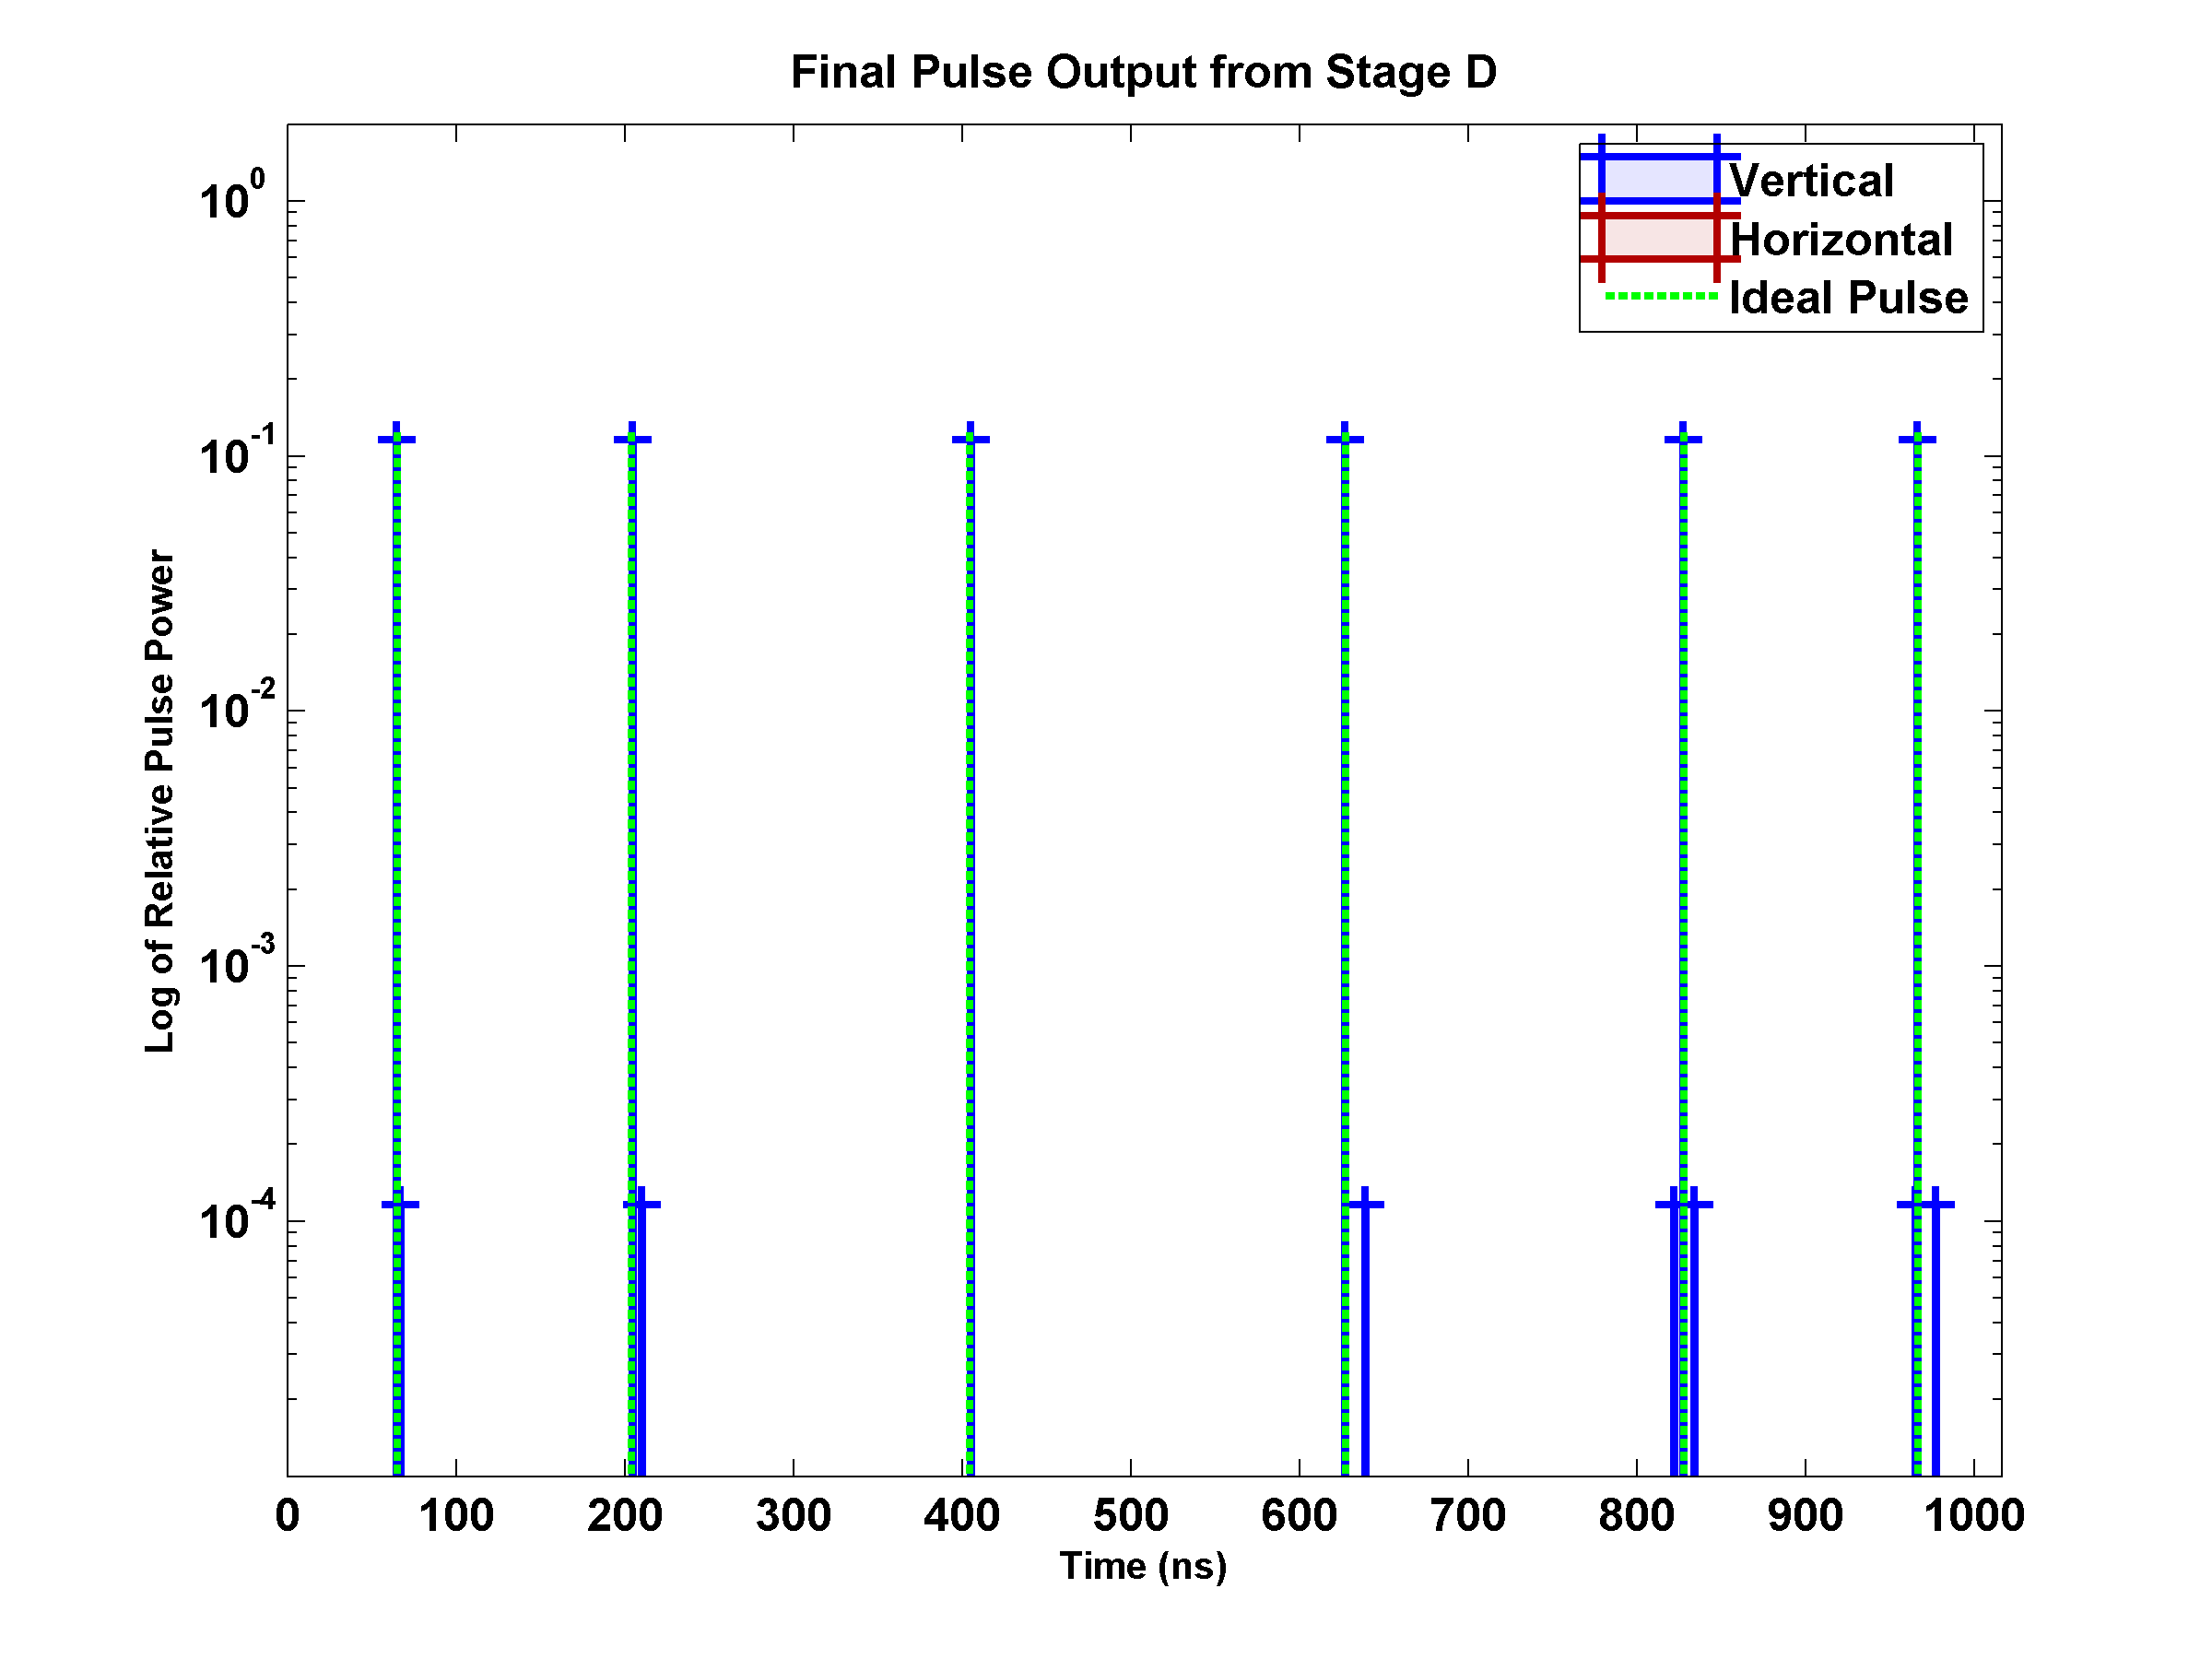
\includegraphics[scale=0.6]{OutputPulse.png}
\caption{This timing diagram shows the output from stage C* of this network, where every pulse aligns with the ideal timing as calculated by the UDD sequence. Note that the additional small pulses from the Pockels Cell inefficiencies are significantly attenuated compared to the true output of the network. In general, the residual pulses are on the order of $10^{-4}$ compared to our output pulses at $10^{-1}$, where these powers are relative to the initial pulse power of 1.  }
\label{fig:timing_E}
\end{figure}


    

\subsubsection{$\pi/2$ Pulses and Compensation Sequences}
\label{sec:pi/2}
One specification not included within the previously detailed Figure \ref{fig:digitizing} is the inclusion of $\pi/2$ pulses at the beginning and end of the sequence. Although not strictly part of the UDD sequence, applying $\pi/2$ pulses before and after the UDD sequence is a necessary part of the experiment.  Essentially, the first $\pi/2$ pulse initializes the state of the quantum dot and the ending $\pi/2$ pulse is used to read out the coherence of the spin\cite{clark_ultrafast_2009}. 

Figure \ref{fig:digitizing_pi2} shows a modification of the digitizing design so that these $\pi/2$ pulses can be produced. At the beginning of the sequence, the first Pockels Cell will let through a pulse destined to become the initializing $\pi/2$ pulse. It will pass through most of the network like any other pulse, until it reaches the third Pockels Cell at B*. Then, this pulse will be directed towards the lower path with horizontal polarization. This causes it to pass through the polarizing beam splitter. From there, it skips the remaining delays as it follows the long red path at C*. When it reaches stage D, the pulse passes through a half-wave plate to correct its polarization and through an attenuator to reduce its amplitude to that of a $\pi/2$ pulse. It is then recombined with the output sequence path. The same thing is done with a pulse at the end of the sequence to produce the ending $\pi/2$ pulse.

While this design modification is necessary to produce these $\pi/2$ pulses, it requires repurposing a branch for the $\pi/2$ pulses, that could otherwise be used as one of the delay combination options. Without this modification in place, pulses from the top and bottom branches leaving the double-passed Pockels Cell could be horizontal or vertical. Now, the horizontal pulse state in the bottom branch must be diverted for $\pi/2$ pulses. Therefore, instead of 16 possible delay combinations, there are only 12. However, by properly optimizing these delays, high precision can still be maintained with this design. The details of optimizing are discussed in Section \ref{sec:optimizing} and a further discussion of precision can be found in Section \ref{sec:error}.

\begin{figure}[H]
\centering
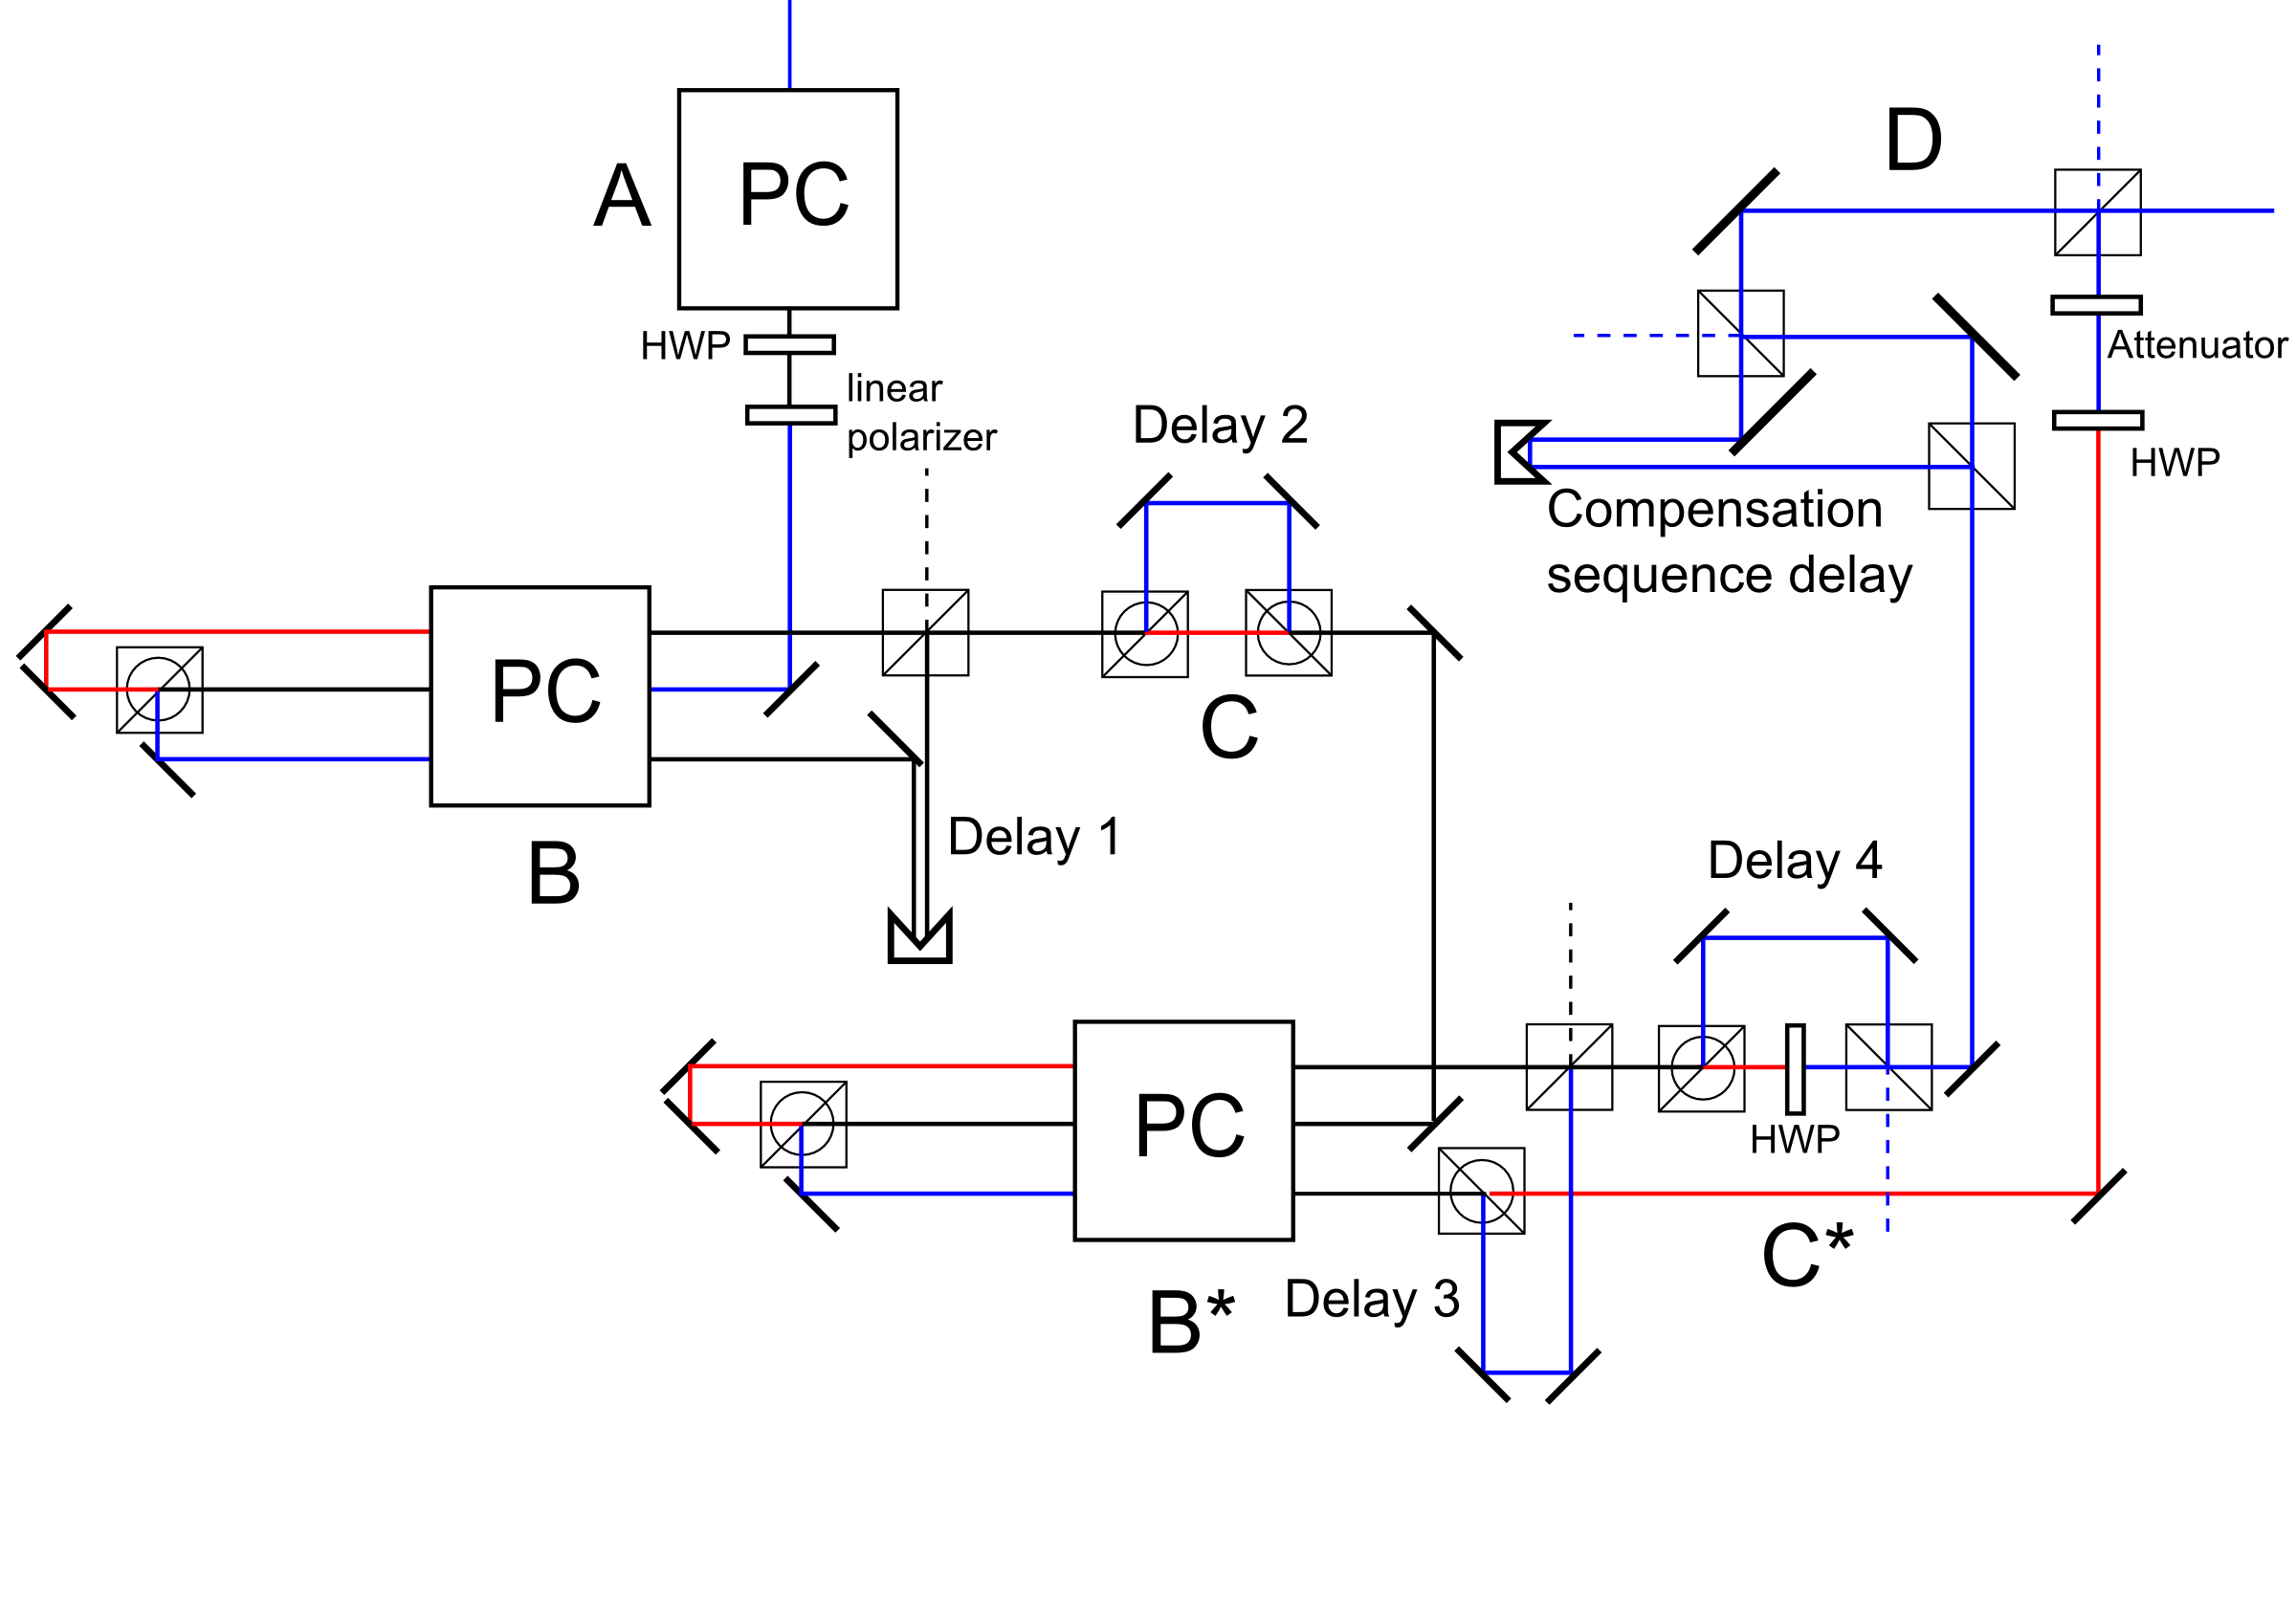
\includegraphics[width=0.9\textwidth]{digitizing_pi2.png}
\caption{This schematic is a digitizing design that can also produce $\pi/2$ pulses at the beginning and end of the sequence, and also implements $\pi/2$ compensation sequences.}
\label{fig:digitizing_pi2}
\end{figure}

Another place where $\pi/2$ pulses are involved are in compensation sequences, described in Section \ref{UDD}. The design shown in Figure \ref{fig:digitizing_pi2} also allows the use of $\pi/2$ compensation sequences. These pairs of $\pi/2$ pulses are created by manipulating the pulses in stage D, after all delays have been applied. All of the $\pi$ pulses in the UDD sequence go through stage D. By splitting the $\pi$ pulses with a beamsplitter, the output pulse is made into two $\pi/2$ pulses of smaller amplitude. One of the pulses is delayed slightly before recombining the paths, creating a pair of $\pi/2$ pulses slightly separated from each other. These pulse pairs improve the noise filtering effects of the sequence\cite{ devitt_requirements_2013}.




\subsection{Design Limitations}
As with any digitizing design, this design necessarily introduces some error when approximating ideal pulse arrival times with the closest available digital pulse. This design can generate up to twelve different delay options, and the delays can be tuned such that the options represent evenly-spaced divisions of the 13-ns repetition rate. In that case, the maximum error for any pulse would be half the spacing between digital pulse options, or 0.54 ns. However, since the ideal times can be computed easily beforehand and the delays can be made adjustable by placing the retroreflectors (or paired mirrors) on a translation stage, the set of delays can be tuned to optimize for a specific choice of $T$ and $n$, thus reducing the digitization error. Even so, the error will unavoidably be larger than for an analog design.

This design is further limited by the switching time of the Pockels Cell, which puts a lower bound on the spacing between consecutive pulses generated by the network. With roughly an 8-ns rise time, the Pockels Cells cannot independently handle two pulses that must be closer than 16 ns. This constraint becomes a problem particularly when attempting to generate pulse sequences for shorter $T$ and larger $n$, as the pulses at the very beginning or end of the sequence may ideally arrive within a few nanoseconds of each other. One possible compensating technique involves setting the delays such that the second Pockels Cell setting for one pulse is the same as the first Pockels Cell setting for the next pulse, which would allow them to access the Pockels Cell simultaneously (note that this would introduce additional constraints on the delay optimization). Alternatively, the design could sacrifice significant precision at the beginnings and ends of pulse sequences in order to function normally.

Lastly, the input pulse rate from the Ti:Sapph laser of one pulse every 13 nanoseconds places a lower limit on $T$ for a given $n$. This design does not split pulses, so for a given length of pulse sequence, $T$, the optical network can only output as many pulses as the laser produces throughout the duration of the sequence. Thus, it cannot generate a complete 30-pulse sequence in only 300 nanoseconds; at least 390 nanoseconds would be required to receive 30 pulses from the input laser.




\section{Test Plan}
\label{sec:test_plan}
This section details the testing plan for the next semester of this project. Next semester's work will involve modifying and improving the simulation tools, as well as some physical testing and component analysis. In addition to any adjustments to the network design or new design ideas, the focus of next semester will be primarily in these areas. 
\subsection{Simulation Advancements}
\label{sec:simadvance}
The areas of advancement for the simulation tools fall under two categories. The first task is to improve the way the tools approximate reality by considering more imperfections. The second task is to improve the user-friendliness of the simulation. 

Currently, the Simulink simulation accounts for imperfections in the Pockels Cell. These imperfections appear throughout the timing diagrams as smaller residual pulses, usually 2-3 orders of magnitude smaller than the main pulses. However, all the rest of the components (i.e. beam splitters, linear polarizers, half-wave plates) are currently modeled with perfect performance. In reality, there will be slight losses, polarization-dependent reflections, and transmissions throughout. It would be valuable to model how all these small imperfections compound together. Additionally, the simulation is simplified to ignore the slight delays as the pulses travel through free space. This instantaneous approximation was helpful in building the model initially, but will need to be considered from here on out. 

While the simulation was helpful in visualizing the network and the modulation of pulses and accounting for imperfections, the Simulink model is currently not very user friendly. Each optical component is contained within a custom block, so arranging the blocks to match a sketch and wiring it up is straightforward. But setting each delay and manually computing and entering the times for the Pockels Cells to be on is tedious. Most testing at this stage hasn't exceeded 6 pulse designs, but once the team explores 20-30 pulse designs, further MATLAB tools to compute the desired timings would be required. This semester the goal was to build a tool that would be usable, but next semester the tool will need to be polished and refined prior to being handed off for further usage. 
\subsection{Physical Testing}

One of the goals for the spring semester will be to try and build some of the most important sections of the digitized design in order to show the viability of a complete system. Given that the team will most likely have access to at most only one Pockels Cell, one of the concepts that will be physically tested is the use of a Pockels Cell to choose between separate branches of the optical network. Of course, the success of this test will rely on a number of the Pockels Cell's properties and their deviations from the ideal, such as the contrast ratio and rise time of the Pockels Cell.     

The team  hopes to characterize the nonidealities of the Pockels Cell, along with those of the other optical components in the network, by designing some simple experiments. For example, we plan to gauge the variance in the splitting ratios of beam splitters by using a power meter to measure the power of the two outgoing beams. Similarly, one can use a power meter to measure an EOM's extinction ratio by measuring the input and output power at minimum transmission.

Moreover, if a partial section of one of the digitized designs is indeed constructed during the spring semester, an ultrafast photodiode can be used at various locations along the beam path in order to characterize the modifications made to the pulse sequence. These experiments coupled with the Simulink simulation tools should allow the team to accurately gauge the performance of the digitized design.


\section{Project Management}
\label{sec:project_managment}
The HRL Clinic Team has developed a work breakdown structure identifying the tasks to be performed, a Gantt chart laying out the milestones and the critical path through the project, and an initial partitioning of the labor among team members. 

\subsection{Work Breakdown Structure}

The work breakdown structure in Figure \ref{fig:WorkBreakDown} shows how the project has been hierarchically subdivided into more manageable tasks. The table shown is the same as initially forecast in the Work Plan. Since completing the Work Plan, the team has found its work projections to be accurate. Computer simulation and design research have taken a primary focus in the fall semester, as was estimated in the Work Plan. The team did not perform any small-scale physical design in the fall semester; however, the team expects most of the physical prototyping to occur in the spring semester, and so those items remain unchanged in the work breakdown structure.

\begin{figure}
\centering
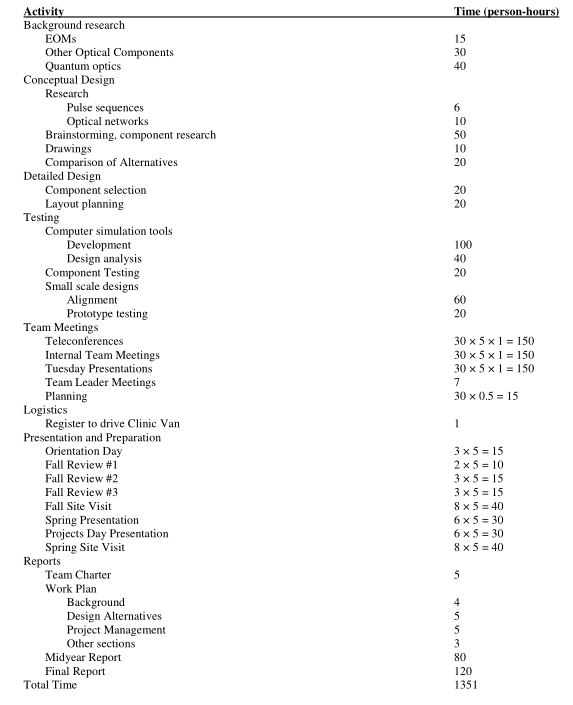
\includegraphics[scale=1.25]{workBreakdown.JPG}
\caption{Work breakdown structure.}
\label{fig:WorkBreakDown}
\end{figure}

\subsection{Schedule}
In the spring semester, the team expects to begin work by integrating the new spring junior with the project in progress. The spring junior will likely work on the simulation tools, which will be the primary work focus for the first month of the semester as the simulation is updated for the current design. The simulation's ability to model non-ideal behavior will be expanded throughout the semester, as well.

Once the current design is finalized, and possibly concurrently with the simulation development, the team intends to begin testing physical components and particular techniques relevant to the design, such as Pockels Cell switching. It will also explore procedures for setting up intricate portions of the design. Near the end of the semester, the team will use the results of its component tests along with additional research to compile component recommendations to include in the final report. The results of the future work outlined above will also be presented in the final report to the liaisons, to be submitted at the end of the spring semester.


\newpage
\bibliographystyle{unsrt}
\bibliography{bibliography}
\bibliographystyle{plain}



\end{document}